\documentclass[12pt,a4paper]{report}
\usepackage[utf8]{inputenc}
\usepackage{geometry}
\usepackage{setspace}
\usepackage{titlesec}
\usepackage{graphicx}
\usepackage{subcaption}
\usepackage{amsmath}
\usepackage{hyperref}
\usepackage{ragged2e}
\usepackage{lmodern}
\usepackage{array}
\usepackage{float}
\usepackage{booktabs}
\usepackage{adjustbox}
\usepackage{longtable}
\usepackage{siunitx}


% Page setup
\geometry{margin=0.7in}
\onehalfspacing
\setlength{\parindent}{1.5em} 
\setlength{\parskip}{0.5em}


% Chapter formatting
\titleformat{\chapter}[display]
  {\bfseries\Large}
  {\filleft\Huge\thechapter}
  {1ex}
  {\titlerule\vspace{1ex}\filright}


% Hyperlink setup
\hypersetup{
    colorlinks=true,
    linkcolor=black,
    urlcolor=blue,
    citecolor=blue
}


\begin{document}
% Title Page
\begin{titlepage}
    \begin{center}
        \large\textbf{GEOPHYSICAL EVALUATION OF SUBSURFACE LAYERS FOR CIVIL}
        \large\textbf{ENGINEERING FOUNDATION USING ELECTRICAL RESISTIVITY METHODS} \\[6.0cm]
        
        \textbf{By:} \\[0.2cm]
        
        \Large\textbf{SURAJUDEEN HADI ADEMOLA} \\[0.1cm]
        \Large\textbf{B.Sc Physics (U.I)} \\[0.1cm]
        \Large\textbf{222814} \\[5.3cm]
        
        \large\textbf{A PROJECT SUBMITTED TO THE DEPARTMENT OF PHYSICS, FACULTY OF SCIENCE,
        UNIVERSITY OF IBADAN, IN PARTIAL FULFILMENT FOR THE AWARD OF BACHELOR IN SCIENCE (B.Sc)
        DEGREE IN PHYSICS} \\[4cm]
        
        \textbf{JANUARY, 2025}
    \end{center}
\end{titlepage}

\pagenumbering{roman}

% Certification
\chapter*{Certification}
\addcontentsline{toc}{chapter}{Certification}  
\justifying  
I certify that this project was carried out under my supervision by \textbf{Surajudeen Hadi Ademola}, with matriculation number \textbf{222814}, of the Department of Physics, Faculty of Science, University of Ibadan.

\vspace{5cm}  

\begin{center}
    \noindent\makebox[7cm]{\hrulefill}  \\  
    \textbf{Dr. A. A. Adetoyinbo}  \\  
    \textbf{B.Sc., M.Sc., Ph.D. (Ibadan)}  \\  
    \textbf{Department of Physics, University of Ibadan}  \\  
    \textbf{(Supervisor)}  
\end{center}

\vspace{3cm}

\begin{center}
    \noindent\makebox[7cm]{\hrulefill}  \\  
    \textbf{Date}  
\end{center}

% Abstract
\chapter*{Abstract}
\addcontentsline{toc}{chapter}{Abstract} 
\justifying
The evaluation of subsurface conditions plays a pivotal role in understanding geological formations and assessing their suitability for various engineering and environmental applications. This project employed an integrated approach using geophysical methods to investigate subsurface properties at an open ground near the University of Ibadan Central Mosque (UI Mosque) and within Abubakar Abdulsalam Hall (AAH), University of Ibadan. A total of 20 Vertical Electrical Soundings (VES) were conducted using the Schlumberger array electrode configuration, with half-current electrode separation (AB/2) ranging from 1 to 55 m for each study area. Additionally, a total of five Profile Constant Separating Transverse (CST) measurements were obtained using the Wenner array electrode configuration, with electrode positions ranging from 0 to 150 m and 0 to 130 m, depending on the profile. These methods were employed to optimize depth-specific and lateral resistivity measurements, providing detailed insights into resistivity variations. The results enabled a comprehensive interpretation of subsurface features such as weak zones, potential failure planes, subsurface layers, soil types, fractures, anomalies, faults, and bedrock characteristics that could impact foundation stability.

The results obtained from the geoelectric sections revealed three primary subsurface geologic layers in both study areas: the topsoil, the weathered layer (comprising clay/sand and laterite), and the fractured basement/fresh bedrock. At the UI Mosque, the resistivity of the topsoil ranged from 220~$\Omega$m to 629.6~$\Omega$m, with a mean value of 367.18~$\Omega$m, and its thickness varied between 0.8~m and 1.1~m. The weathered layer exhibited a resistivity range of 60~$\Omega$m to 231~$\Omega$m, with a mean value of 110.61~$\Omega$m, and its thickness and depth ranged from 1.8~m to 3.0~m and 4.0~m to 22~m, respectively. The resistivity of the delineated fractured and fresh bedrock ranged from 27.7~$\Omega$m to 449.3~$\Omega$m, although the depth of the fresh bedrock was undetermined. The resistivity and thickness of the subsurface layers indicate the suitability of the area for light to moderate civil engineering foundations. However, the presence of fractured zones may require further geotechnical evaluation for heavy structures.

Also, at the AAH site, the resistivity of the topsoil ranged from 186.9 Ωm to 1222.0 Ωm, with a mean value of 422.5 Ωm, and its thickness varied between 0.5 m and 1.0 m. The weathered layer exhibited a resistivity range of 13.6 Ωm to 70.0 Ωm, with a mean value of 29.6 Ωm, and its thickness and depth ranged from 1.4 m to 9.9 m and 1.9 m to 10.9 m, respectively. The resistivity of the delineated fractured and fresh bedrock ranged from 166.7 Ωm to 834.5 Ωm. The resistivity and thickness of the subsurface layers indicate in this area showed that these fractured zones could indicate potential instability or the presence of water-bearing layers, which may affect the load-bearing capacity of the subsurface materials. Therefore, a detailed geotechnical evaluation, including borehole drilling and core sampling, is recommended to assess the integrity of the bedrock and ensure the safety and stability of any heavy structures planned for the site.

% Dedication
\chapter*{Dedication}
\addcontentsline{toc}{chapter}{Dedication} 
\justifying
I dedicate this project to the Almighty God, whose wisdom, strength, and guidance have been my source of inspiration throughout this academic journey.  To my beloved parents, whose unwavering love, sacrifices, and encouragement have shaped my path and fueled my ambition. Your prayers and support have been the foundation of my success.  


% Acknowledgements
\chapter*{Acknowledgements}
\addcontentsline{toc}{chapter}{Acknowledgements}
\justifying
First and foremost, I express my profound gratitude to Almighty God for granting me the strength, wisdom, and perseverance to complete this project successfully.  

I would like to extend my sincere appreciation to my supervisor, \textbf{Dr. Adedeji Adegoke Adetoyinbo}, for his invaluable guidance, and unwavering support throughout this project. My sincere appreciation also to \textbf{Prof. Adekunle Kazeem Bello}, his expertise and mentorship have been instrumental in shaping this work.  

A special appreciation goes to my family for their endless love, prayers, moral and financial support. Their unwavering belief in my abilities has been a constant source of motivation.  

I am also thankful to my friends most especially \textbf{David Tolulope} and colleagues for their encouragement and assistance, as well as for creating an environment of collaboration and learning.

Finally, I acknowledge the contributions of everyone who, in one way or another, played a role in the successful completion of this project.  

% List of Figures
\listoffigures
\addcontentsline{toc}{chapter}{List of Figures}

% List of Tables
\listoftables
\addcontentsline{toc}{chapter}{List of Tables}

% Table of Contents
\tableofcontents

\newpage

\pagenumbering{arabic}

% Chapter 1: INTRODUCTION
\chapter{CHAPTER 1: INTRODUCTION}
\numberwithin{equation}{chapter}

\section{Background to the Study}

Building failures, a prevalent issue in various regions, often result from poor soil conditions, inadequate site investigations, and a lack of understanding of the underlying subsurface structure. \textbf{(Amadi, \textit{et al.,} 2012)} highlight that improper foundation designs and insufficient knowledge of the structural distribution of subsurface layers are leading contributors to such failures. Also, \textbf{(Kværna and \textbf{Øygarden} 2006)} emphasized that soil instability often caused by moisture fluctuations, plays a significant role in compromising the structural integrity of buildings. To mitigate these risks, comprehensive geophysical surveys are vital for analyzing the properties of the ground before construction.

Recent studies have expanded the scope of geophysical methods like Vertical Electrical Sounding (VES) and Constant Separation Traversing (CST) to include subsurface mapping, groundwater exploration, and geotechnical evaluations. \textbf{(Adetoyinbo, \textit{et al.,} 2023)}, in their work published in the \textit{International Journal of Scientific and Applied Research}, used VES to assess groundwater potential and subsurface characteristics in Idi-Ayunre, Ibadan. Their study identified significant geological features, such as fracture zones and aquifer units, revealing areas with low groundwater prospects. Similarly, \textbf{(Ogunseye, \textit{et al.,} 2022)}, in their work published in the \textit{Journal of Environmental Studies}, analyzed the geochemical properties of soils in Mokola, Ibadan, using soil samples and laboratory tests. Their findings highlighted the presence of heavy metal contamination, emphasizing its potential impact on groundwater quality and the importance of including geochemical assessments in subsurface investigations. The application of Constant Separation Traversing (CST) has also gained significant attention for its role in evaluating lateral resistivity variations and detecting geological discontinuities. \textbf{(Anomohanran, \textit{et al.,} 2016)} applied CST to investigate lateral subsurface variations in the Niger Delta region, highlighting its effectiveness in detecting faults, fractures, and lithological boundaries that may compromise the stability of engineering foundations. Their findings demonstrated how CST complements VES by providing lateral profiling of resistivity, offering a more comprehensive understanding of subsurface conditions. Furthermore, \textbf{(Ismaila, \textit{et al.,} 2019)} used CST in combination with VES to assess subsurface layers for road construction projects in Ilorin, Nigeria. Their work revealed significant variations in soil composition and resistivity, emphasizing the need for lateral resistivity profiling in regions with heterogeneous geological settings.

Geophysical surveys, including VES and CST, are particularly significant in regions where soil heterogeneity poses risks to construction activities. For example, \textbf{(Agada, Ibuot, and Oseghale, \textit{et al.,} 2013)} investigated subsurface characteristics in an area prone to structural failures. Their findings revealed that geological discontinuities, such as fractures and dislocations, were primary contributors to differential settlements and structural disintegration. This underscores the importance of employing methods like VES and CST, which can delineate subsurface features with precision. Electrical resistivity surveys have emerged as a popular method in geotechnical investigations due to their high spatial resolution, cost-effectiveness, and non-destructive nature. This method measures the ability of subsurface materials to conduct electrical currents, enabling the identification of various layers, voids, fractures, and lithological features. As noted by \textbf{(Griffiths and Barker 1993)}, and corroborated by \textbf{(Soupisos, \textit{et al.,} 2006)}, these surveys provide critical data that can prevent construction failures by ensuring that foundation designs align with the physical and structural characteristics of the site.

Furthermore, \textbf{(Warner 2004)} and \textbf{(Ozeqin, \textit{et al.,} 2017)} emphasized that geophysical techniques are indispensable tools for assessing the bearing capacity of soils. These methods enable civil engineers to identify areas of concern, such as seepage zones and clayey substrata, which can cause excessive settlement and cracking in buildings. By incorporating such techniques into site investigations, construction projects can significantly reduce the risks associated with geotechnical failures. In practical terms, electrical resistivity methods, including VES and CST, have been successfully applied in various engineering projects to identify and map subsurface structures. According to \textbf{(Lapenna, \textit{et al.,} 2005)}, these methods are invaluable for delineating depth variations, subsurface discontinuities, and lithological interfaces that may affect foundation stability. In addition to their technical benefits, they offer a cost-effective solution compared to traditional drilling methods, making them accessible for large-scale geotechnical investigations.

In summary, the integration of Vertical Electrical Sounding (VES) and Constant Separation Traversing (CST) represents an innovative approach to geotechnical site investigation by addressing challenges related to subsurface heterogeneity and providing insights into lateral and vertical variations, these methods mitigate risks of construction failure. This study employs these techniques to evaluate the geotechnical characteristics of the subsurface within the study area, contributing to safer and more sustainable civil engineering practices.

\section{Research Problem}
Inadequate knowledge of subsurface conditions remains a critical factor contributing to building failures, particularly in regions with complex and heterogeneous geological settings. Engineers often face challenges in accurately assessing subsurface characteristics, which leads to poorly designed foundations that are unable to prevent excessive settling, structural cracking, or outright collapse. Despite advancements in construction technology, many civil engineering projects still suffer from cost overruns and safety concerns stemming from improper site investigations.
While geophysical methods like Vertical Electrical Sounding (VES) and Constant Separation Traversing (CST) have demonstrated significant potential in subsurface characterization, their application in civil engineering foundation designs remains underexplored. This gap in the integration of effective site investigation techniques results in a lack of precise and actionable data, which not only compromises structural stability but also incurs substantial economic and safety risks. By addressing this issue, the study aims to highlight how the use of advanced geophysical methods can bridge this gap, mitigate construction-related challenges, and enhance sustainable engineering practices. This research focuses on leveraging VES and CST to provide comprehensive subsurface information, ensuring improved construction outcomes and safer foundation designs.

\section{Aim and Objectives}
\subsection{Aim of the Study}
The aim of this project is to evaluate the subsurface layers for civil engineering foundation design by employing electrical resistivity methods, specifically Vertical Electrical Sounding (VES) with Schlumberger configuration and Constant Separation Traversing (CST) with Wenner configuration, aiming to provide actionable insights for foundation stability.

\subsection{Objectives of the Study}
The specific objectives of this study are to:
\begin{itemize}
    \item Map the subsurface layers and determine their resistivity values using VES and CST methods.
    \item Identify weak zones, fractures, and groundwater presence that may affect the stability of civil engineering foundations.
    \item Analyze the depth, thickness, and resistivity of subsurface layers to assess their suitability for various foundation types.
    \item Detect lateral variations such as faults, fractures, or discontinuities using CST to complement the vertical subsurface evaluation.
    \item Correlate resistivity values with lithological and geotechnical properties, such as soil type, compaction, and strength.
    \item Combine VES and CST data to generate 3D visualization of the subsurface using specialized geophysical software, enhancing the interpretation and understanding of subsurface features.
    \item Provide engineering recommendations for foundation design based on geophysical findings, ensuring safety, cost-efficiency, and structural stability in the study area.
\end{itemize}

\section{Justification of the Study}
Understanding subsurface layers is essential for civil engineering foundation design, as inadequate knowledge can lead to structural failures, safety risks, and financial losses. The use of Vertical Electrical Sounding (VES) and Constant Separation Traversing (CST) offers a powerful, cost-effective, and non-invasive approach to addressing these challenges.

Previous studies, such as \textbf{(Coker 2012)} in Akobo area of Ibadan and \textbf{(Adagunodo, \textit{et al.,} 2013)} in Oniye, Southwestern Nigeria, demonstrated the utility of VES for groundwater exploration and fracture detection. Similarly, research by \textbf{(Farinde, \textit{et al.,} 2015)} focused on integrating geophysical and geotechnical methods for road construction at the University of Ibadan. However, these studies often emphasized resource exploration or general geotechnical characterizations rather than specifically addressing civil engineering foundation requirements.

Regions with heterogeneous soil conditions, such as Ibadan, require tailored and localized geophysical evaluations to mitigate risks like differential settlement and soil instability. While earlier works have provided valuable geological insights, a significant gap remains in leveraging these findings for actionable recommendations in foundation design.

This study aims to fill this gap by explicitly integrating VES and CST methods to evaluate the lithological and structural characteristics of subsurface layers. VES will focus on vertical resistivity profiling, while CST will provide complementary lateral resistivity variations, making it possible to detect faults or fractures that could compromise foundation stability. By correlating resistivity data with geotechnical properties, this research delivers practical insights into soil properties, lithological variations, and structural integrity, enhancing the safety and cost-efficiency of construction practices.

Unlike previous studies, this project emphasizes civil engineering applications, offering a novel approach to geophysical evaluations tailored for foundation design. The findings will contribute to safe and sustainable construction practices, bridging the gap between geophysical insights and practical engineering solutions in complex geological settings.

\section{Geophysical Investigation}
In this project work, the geophysical survey was carried out using Vertical Electrical Sounding (VES) with the Schlumberger array electrode configuration and Constant Separation Traversing (CST) with the Wenner array electrode configuration. A total of \textbf{20 VES} profiles and \textbf{5 CST} profiles were conducted. The coordinates of the points in the selected area were taken, and the results were collated. The electrical resistivity method involves injecting current into the ground and measuring the resulting potential difference to determine subsurface resistivity variations. These variations help delineate different geological layers, assess lithological properties, and detect fractures or faults.

\section{Geological Settings}

\subsection{The Study Location}
Nigeria, located in West Africa, offers a rich and varied geological tapestry for geophysical research on subsurface layers, particularly for civil engineering foundations. The country's geology ranges from the ancient crystalline basement complex in the southwest, composed of migmatites, gneisses, and granites, to several significant sedimentary basins like the Niger Delta, the Benue Trough, and the Chad Basin. The basement complex's extensive weathering creates a regolith that significantly impacts foundation stability, necessitating thorough geophysical investigation to understand its depth and characteristics. The sedimentary basins, especially the Niger Delta, present complex stratigraphy with layers of sand, silt, and clay, which have substantial implications for foundation design due to their variable thickness and composition. Hydrogeologically, Nigeria shows diversity with groundwater confined to fractured and weathered zones in the basement areas, contrasting with the broader aquifers in sedimentary regions, affecting soil moisture and stability. Structurally, the presence of faults, folds, and fractures across the nation dictates the subsurface's response to structural loads, crucial for avoiding issues like differential settlement. Even within these broad geological zones, local variability due to tectonic activity, erosion, and sediment deposition makes each site unique, particularly in areas like Ibadan where soil conditions can be highly heterogeneous.

Previous geophysical studies in Nigeria have laid a foundation for understanding how techniques like VES and CST can be applied to map and interpret these geological features for civil engineering purposes on how to ensure the safety and sustainability of civil engineering projects through geophysical evaluation of subsurface conditions. \\

\begin{figure}[H]
    \centering
    \includegraphics[width=0.7\textwidth]{Nigeria_Study_Country.png}
    \caption{Map showing Nigeria from the World Map generated using QGIS.}
\end{figure}

\subsection{The Study Area}

The geophysical investigation for this study was conducted across two distinct locations within Ibadan North Local Governement at the University of Ibadan, Oyo State, Nigeria. This study area lies within the southwestern part of Nigeria, each chosen to represent different geological and soil conditions pertinent to civil engineering foundation design.

\subsubsection{\textbf{First Location:}}
Located at Emotan Lane in an open site at the University of Ibadan Central Mosque (UI Mosque), Ibadan, with coordinates 7.44662° N, 3.89960° E, this site lies within the southwestern part of Nigeria. This area is characterized by the crystalline basement complex, typical of the region, with significant weathering that could impact foundation stability. Here, 10 Vertical Electrical Soundings (VES) were executed using the Schlumberger electrode configuration, and 3 Constant Separation Traversing (CST) profiles were conducted with the Wenner electrode configuration.

\subsubsection{\textbf{Second Location:}}
The second investigation site is at Appleton Road in Abubakar Abdulsalam Hall (AAH), University of Ibadan, with coordinates 7.43933° N, 3.89449° E. This location also represents the geological complexity of the area, featuring a mix of basement rocks with potential for varying soil compositions due to its proximity to different geological features. This site was chosen to assess how these conditions affect foundation stability and to understand the variability in soil composition. Here, 10 VES were similarly carried out, and 2 CST profiles were established.

Both areas were selected to provide a comprehensive understanding of the subsurface conditions within the University of Ibadan campus, ensuring the findings can be directly applicable to civil engineering practices in similar geological settings. The precise coordinates of these sites were meticulously recorded to enable accurate geophysical surveying and to facilitate future reference or validation of the study results.

\begin{figure}[H]
    \centering
    \begin{subfigure}[t]{0.89\textwidth}
        \centering
        \includegraphics[width=\textwidth]{Oyo_Study_Location.png}
        \caption{Map showing Oyo State Region from Nigeria Map.}
        \label{fig:Oyo Study Location}
    \end{subfigure}
    \vspace{1cm} 
    \begin{subfigure}[t]{1.0\textwidth}
        \centering
        \includegraphics[width=\textwidth]{UI_Study_Area_Map.png}
        \caption{Map of Ibadan North highlighting the University of Ibadan Study Area.}
        \label{fig:UI Study Area}
    \end{subfigure}
    
    \caption{Combined maps for the study location and study area generated by QGIS.}
    \label{fig:Combined Maps}
\end{figure}

\begin{figure}[H]
    \centering
    \begin{subfigure}[t]{0.9\textwidth}
        \centering
        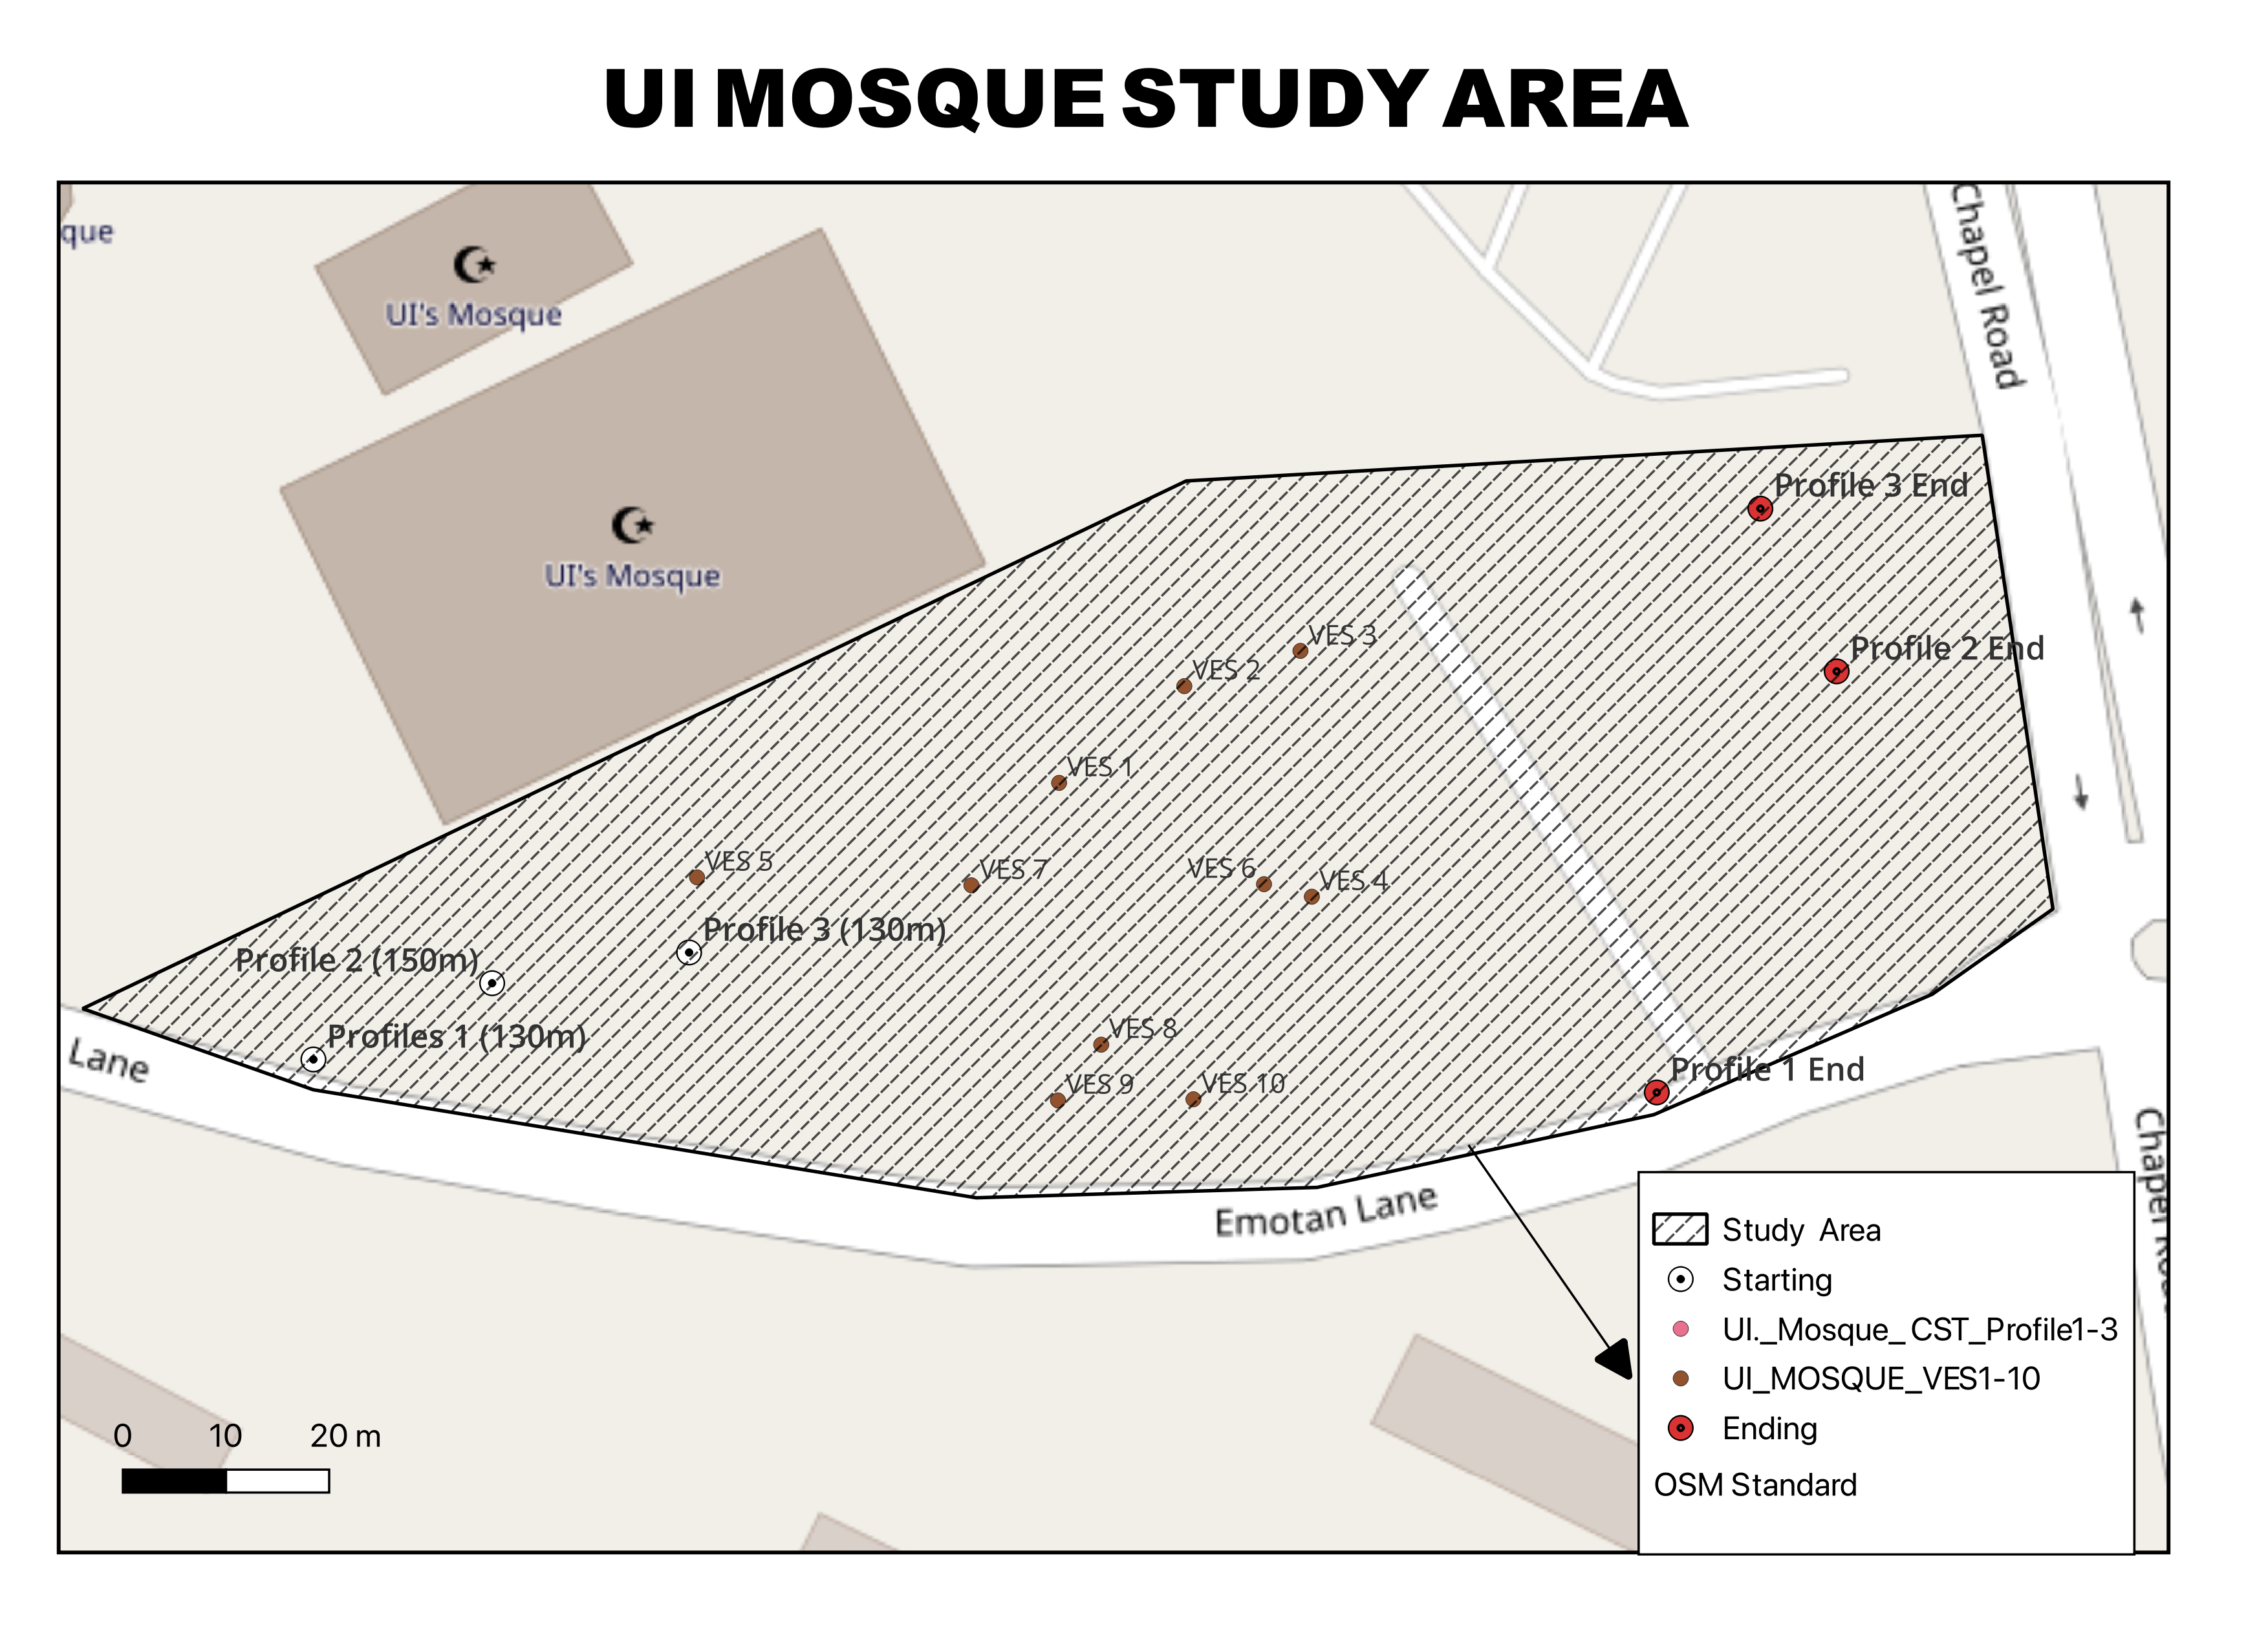
\includegraphics[width=\textwidth]{UI_Mosque_Map_Layout.png}
        \caption{\textbf{Coordinates:} 7.44662° N, 3.89960° E.}
        \label{fig:UI Mosque Study Area}
    \end{subfigure} 
    \begin{subfigure}[t]{1.0\textwidth}
        \centering
        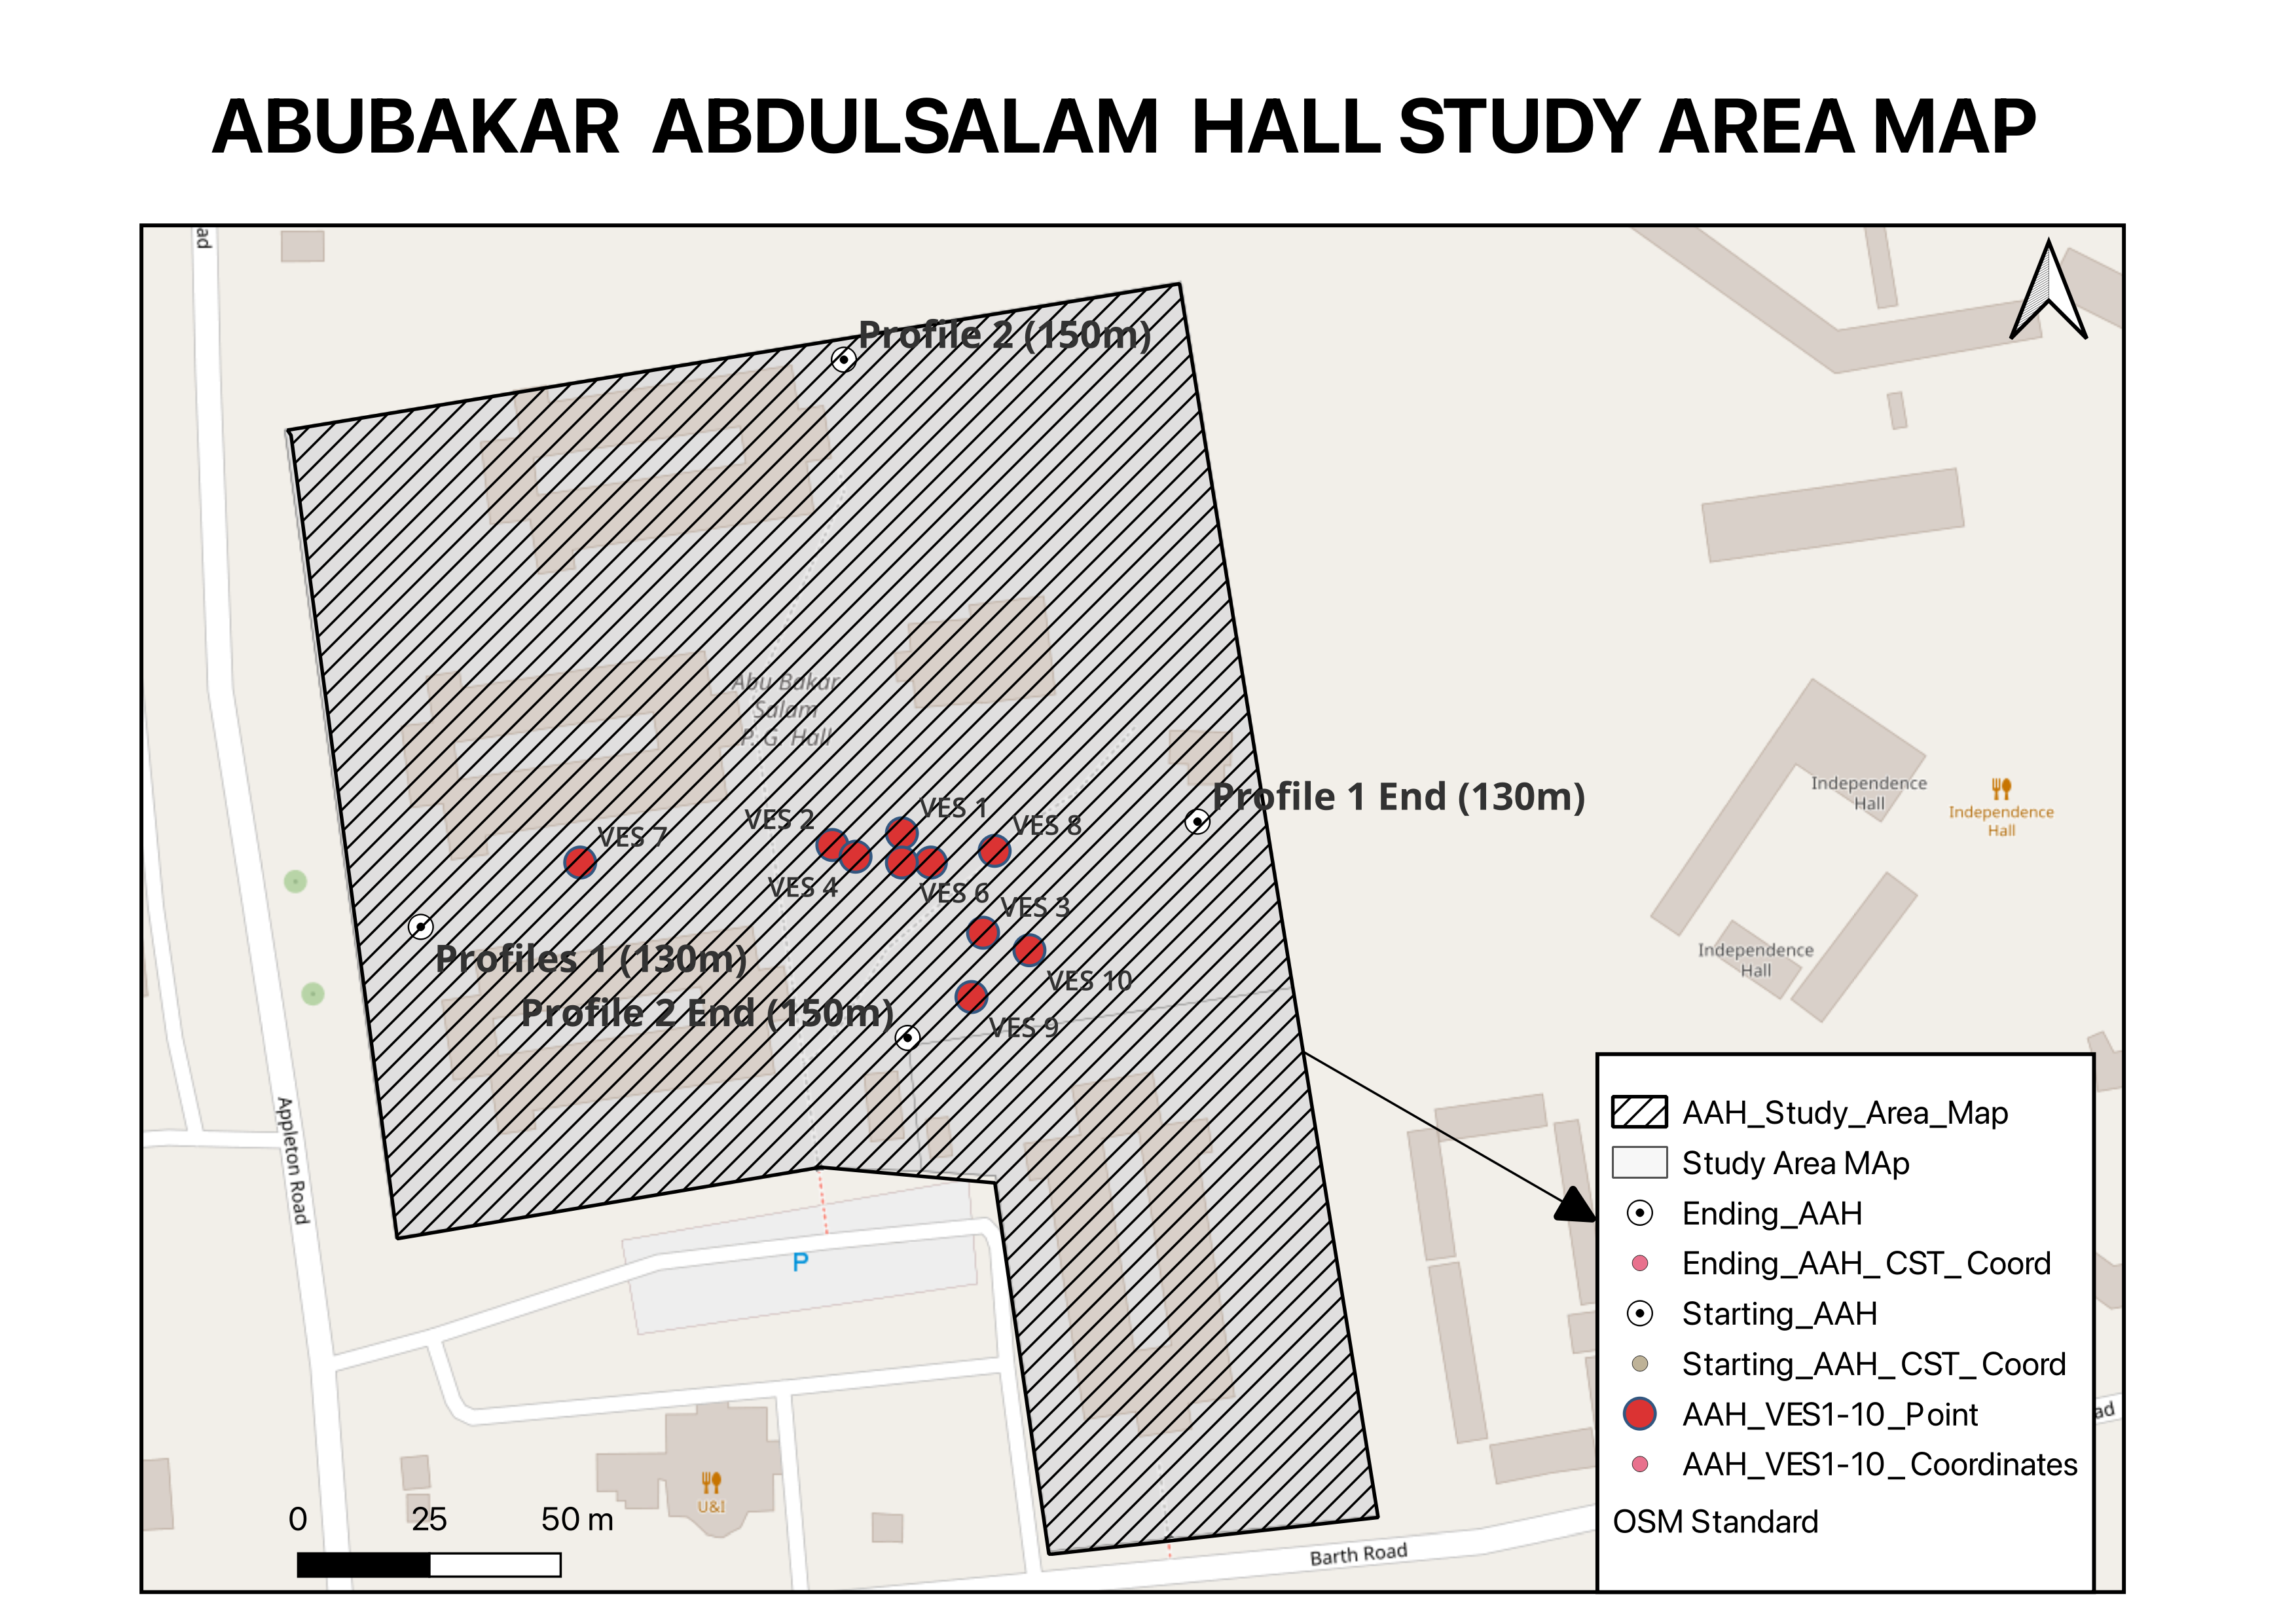
\includegraphics[width=\textwidth]{AAH_Map_Layout.png}
        \caption{\textbf{Coordinates:} 7.43933° N, 3.89449° E.}
        \label{fig:AAH Study Area}
    \end{subfigure}
    \caption{Combined maps for the study areas generated by QGIS.}
    \label{fig:Combined Study Areas}
\end{figure}

\newpage
\section{Outline of the Thesis}
This thesis is organized into five chapters:
\begin{itemize}
    \item Chapter 1: Introduction, including the aims, objectives, the study location and area including the significance of the study.
    \item Chapter 2: Literature Review, providing a detailed discussion of previous research, theoretical principles, applications, challenges and the limitations of the study.
    \item Chapter 3: Materials and Methods of the research and analysis.
    \item Chapter 4: The results, analysis, combination of VES and CST and further discusion.
    \item Chapter 5: Summary, Conclusion and Recommendations
\end{itemize}
References and acronyms were also included at the end of the project

% Chapter 2: LITERATURE REVIEW
\chapter{CHAPTER 2: LITERATURE REVIEW}
\numberwithin{equation}{chapter}

\section{Introduction to Geophysical Methods in Civil Engineering}
Geophysical methods are generally non-invasive or non destructive methods long used in the construction industry for investigation of the subsurface. Principally, these are used for the detection of geologic anomalies such as cavities and voids, detection of buried pipes and other utilities, detection of water bearing aquifers for well development, exploitation of quarries and in determining soil stratification or layering. In addition, the methods provide a means for verifying as constructed pavement thicknesses in a continuous unbroken image of the pavement structural configuration or determining rebar embedment and layout non destructively.

The use of Geophysical methods confers advantages as they generally speed up the process of investigation, provide continuous streams of information not otherwise available in discrete sampling or invasive procedures and give advance information on what to expect for a given locality before a more detailed and costly soil exploration is even planned. Thus Geophysical methods are a force multiplier for the engineer and allow the user to identify potential problem areas or target areas even before the start of a detailed Soil Exploration program.

Geophysical methods are not a replacement to a detailed soil exploration program; rather they augment these programs to yield more meaningful and area extensive but more intensive information at the fraction of the time and cost. Geophysical Methods have been around for quite some time. These are non invasive procedures employed in order to determine subsurface soil conditions and geologic anomalies such as cavities and voids or buried objects such as pipelines. Geophysical methods are used for various purposes in Civil Engineering Investigation of the subsurface. The advent of high speed computers and fast signal processors have vastly improved the technology and resulted in increased reliability and signal clarity in the use of these methods.

\textbf{Emilio M. \textit{et al.,}} in their Paper titled \textit{Geophysical Methods in Civil Engineering - Practical Applications} presented their local practical experience in the deployment of Geophysical methods and equipment to address and provide solutions to various practical problems where conventional approaches may not give adequate information or may not provide it in a faster or more accurate way. Geophysical methods address the need for more information compared to conventional borings, these are not substitute to actual soil borings particularly when soil design parameters (strength and compressibility) are needed. However, borings may provide only limited discrete information points or are limited because of budgetary restrictions while Geophysical methods may provide a continuous data stream or even three dimensional images of the desired target of interest. Thus these two methods are complementary and would provide a more meaningful information record when done together or when augmented by each other. These methods are not a substitute for detailed borings except for specific objectives which do not require strength characterization or design strength or compressibility parameters, they can sometimes yield more meaningful results and thus corroborate results of other methods.

\section{Overview of Geophysical Techniques}
Geophysical techniques offer innovative, non-invasive solutions for subsurface investigations, which are crucial in civil engineering projects. These methods provide reliable data on subsurface conditions, enabling engineers to make informed decisions regarding foundation designs, groundwater exploration, and the detection of subsurface anomalies. Among the most prominent techniques are \textbf{Ground Penetrating Radar (GPR)}, \textbf{Seismic Refraction}, and \textbf{Electrical Resistivity Methods}, each with unique principles, applications, and limitations.

\subsection{Ground Penetrating Radar (GPR)}
Ground Penetrating Radar (GPR) is a geophysical method that uses electromagnetic radar pulses to investigate the subsurface. Initially developed for military applications, such as detecting mines and buried weapons, GPR has become an essential tool in civil engineering due to its ability to provide high-resolution, real-time subsurface imaging.

\subsubsection{Principle of Ground Penetrating Radar}
GPR operates by transmitting electromagnetic radar impulses into the ground. The radar waves are reflected or absorbed based on the material's stiffness, moisture content, and composition. Reflected signals are captured by a receiving antenna and processed in real time to produce a subsurface image. The depth of investigation is inversely proportional to the radar frequency: higher frequencies provide better resolution at shallow depths, while lower frequencies are used for deeper penetration.

\subsubsection{Applications of Ground Penetrating Radar}
In a highway construction project, GPR is used to measure pavement thickness to millimeter precision, enabling dispute resolution and ensuring compliance with quality standards. GPR is versatile, with applications including:
\begin{itemize}
    \item Detection of cavities, voids, and geologic anomalies.
    \item Locating buried objects, such as pipelines, rebar, and archaeological artifacts.
    \item Environmental scanning for waste landfill detection.
    \item Measuring roadway and pavement thickness for quality assurance.
    \item Structural assessment of concrete to detect embedded objects.
\end{itemize}

\subsubsection{Inherent Limitations of Ground Penetrating Radar}
\begin{itemize}
    \item Signal attenuation in conductive soils, such as clay, reduces penetration depth.
    \item The method's resolution decreases with increasing depth.
    \item Interpretation requires expertise and can be affected by noise and interference.
\end{itemize}

\subsection{Seismic Refraction Methods}
In a slope stabilization project, seismic refraction identified fault zones and sloping bedrock, enabling engineers to optimize foundation placement and reduce risks of structural failure. Seismic refraction is a method that utilizes shock waves to analyze subsurface structures and material properties. It is particularly effective for investigating stratigraphy and mechanical properties of soils and rocks.

\subsubsection{Principle of Seismic Refraction Methods}
Shock waves are generated by striking a steel plate with a hammer or using explosives. These waves travel through the ground, refracting and reflecting at material boundaries. Geophones positioned along a linear spread detect these waves, and their arrival times are recorded by a seismograph. The velocity of wave propagation provides insights into the stiffness and composition of subsurface layers.

\subsubsection{Applications of Seismic Refraction Methods}
\begin{itemize}
    \item Determining subsurface stratification and soil stiffness.
    \item Identifying faults, fractures, and cavities.
    \item Assessing sloping bedrock and geologic anomalies.
    \item Ensuring foundation stability in construction projects.
\end{itemize}

\subsubsection{Field Procedure of Seismic Refraction Methods}
A typical seismic refraction layout, known as a “spread,” involves 12 to 24 geophones. Multiple "shots" are conducted to ensure thorough coverage and accurate detection of subsurface anomalies. Each shot provides detailed data on layer characteristics and velocities.

\subsection{Electrical Resistivity Methods}
Surface electrical resistivity surveying is based on the principle that the distribution of electrical potential in the ground around a current-carrying electrode depends on the electrical resistivities and distribution of the surrounding soils and rocks.  The usual practice in the field is to apply an electrical direct current (DC) between two electrodes implanted in the ground and to measure the difference of potential between two additional electrodes that do not carry current.  Usually, the potential electrodes are in line between the current electrodes, but in principle, they can be located anywhere.  The current used is either direct current, commutated direct current (i.e., a square-wave alternating current), or AC of low frequency (typically about 20 Hz).  All analysis and interpretation are done on the basis of direct currents.  The distribution of potential can be related theoretically to ground resistivities and their distribution for some simple cases, notably, the case of a horizontally stratified ground and the case of homogeneous masses separated by vertical planes (e.g., a vertical fault with a large throw or a vertical dike).  For other kinds of resistivity distributions, interpretation is usually done by qualitative comparison of observed response with that of idealized hypothetical models or on the basis of empirical methods.

Mineral grains comprised of soils and rocks are essentially nonconductive, except in some exotic materials such as metallic ores, so the resistivity of soils and rocks is governed primarily by the amount of pore water, its resistivity, and the arrangement of the pores.  To the extent that differences of lithology are accompanied by differences of resistivity, resistivity surveys can be useful in detecting bodies of anomalous materials or in estimating the depths of bedrock surfaces.  In coarse, granular soils, the groundwater surface is generally marked by an abrupt change in water saturation and thus by a change of resistivity.  In fine-grained soils, however, there may be no such resistivity change coinciding with a piezometric surface.  Generally, since the resistivity of a soil or rock is controlled primarily by the pore water conditions, there are wide ranges in resistivity for any particular soil or rock type, and resistivity values cannot be directly interpreted in terms of soil type or lithology.  Commonly, however, zones of distinctive resistivity can be associated with specific soil or rock units on the basis of local field or drill hole information, and resistivity surveys can be used profitably to extend field investigations into areas with very limited or nonexistent data.  Also, resistivity surveys may be used as a reconnaissance method, to detect anomalies that can be further investigated by complementary geophysical methods and/or drill holes.

The electrical resistivity method has some inherent limitations that affect the resolution and accuracy that may be expected from it.  Like all methods using measurements of a potential field, the value of a measurement obtained at any location represents a weighted average of the effects produced over a large volume of material, with the nearby portions contributing most heavily.  This tends to produce smooth curves, which do not lend themselves to high resolution for interpretations.  Another feature common to all potential field geophysical methods is that a particular distribution of potential at the ground surface does not generally have a unique interpretation.  Although these limitations should be recognized, the non-uniqueness or ambiguity of the resistivity method is scarcely less than with the other geophysical methods.  For these reasons, it is always advisable to use several complementary geophysical methods in an integrated exploration program rather than relying on a single exploration method. A single resistivity measurement requires four electrodes coupled to the ground and provides the apparent resistivity of the materials located between the potential electrodes. This surveys typically utilize multiple electrode pairs arranged in various configurations (i.e., spatial geometries), chosen based on site parameters and survey objectives \textbf{(Binley, 2015)}.

\section{Theoretical Background of Electrical Resistivity Methods}

\subsection{General Principles of Electrical Resistivity Methods}
The principle of electrical resistivity is based on Ohm's Law, which relates the flow of electric current through a material to its resistivity. Subsurface materials exhibit varying resistivity based on their composition, moisture content, and porosity. Conductive materials such as clays and water-saturated zones show low resistivity, while compact, dry rocks display high resistivity values. This variation allows for the characterization of subsurface layers.

\subsubsection{Principle of Resistivity}
Ohm's Law relates voltage ($V$), current ($I$), and resistance ($R$) through the equation:
\begin{equation}
    R = \frac{V}{I}
\end{equation}
In the context of subsurface investigations, resistivity ($\rho$) is calculated by considering the geometric dimensions of the material:
\begin{equation}
\rho = R \frac{A}{L}
\end{equation}

where:
\begin{itemize}
    \item $\rho$ = Resistivity of the material ($\Omega \cdot m$),
    \item $R$ = Measured resistance ($\Omega$),
    \item $A$ = Cross-sectional area of the material ($m^2$),
    \item $L$ = Length of the material ($m$).
\end{itemize}

\subsubsection{Key Concept:}  
Conductive materials like clays and water-saturated zones have low resistivity, while dry, compact rocks and non-porous materials exhibit high resistivity. This contrast enables the detection of geological features such as aquifers, fractures, and stratigraphic boundaries.

\subsection{Electric Current Flow in Subsurface Materials}
When an electric current is introduced into the subsurface, it spreads radially through the soil or rock. The current's behavior depends on the material's resistivity, with high-resistivity materials offering greater resistance to current flow and low-resistivity materials allowing easier passage. The electric field generated by the current is measured using potential electrodes.

\subsubsection{Equation for Current Density:}
\begin{equation}
J = \sigma E
\end{equation}
where:
\begin{itemize}
    \item $J$ = Current density ($A/m^2$),
    \item $\sigma$ = Electrical conductivity ($1/\rho$, $S/m$),
    \item $E$ = Electric field intensity ($V/m$).
\end{itemize}

\begin{figure}[H]
    \centering
    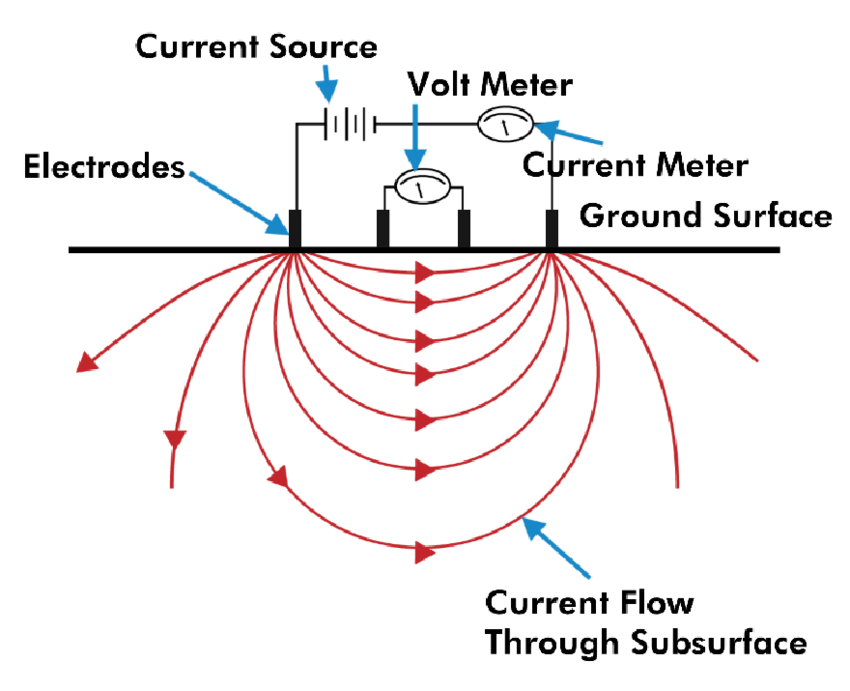
\includegraphics[width=0.76\textwidth]{current-flow.png}
    \caption{Diagram illustrating electrical current flow through subsurface}
\end{figure}

\subsection{Electrical Field and Potential}
When current is injected into the subsurface, it creates an electrical field. The potential difference ($\Delta V$) measured across two points is influenced by the resistivity of the intervening materials. Equipotential lines and current flow lines provide a visual representation of how the electrical field is distributed within the subsurface, aiding in the interpretation of resistivity data.

Coulomb established that the force of attraction or repulsion between two charged spheres is proportional to the product of the individual electric fields and inversely proportional to the square of the distance between the centers of the spheres. The electric field of a charge is a force \(\mathbf{F}\) exerted on another unit charge using Coulomb's law.

The force \(\mathbf{F}\) is given by:

\begin{equation}
\mathbf{F} \propto \frac{q_1 q_2}{r^2}
\end{equation}

Introducing the constant of proportionality \(k_e\), the equation becomes:

\begin{equation}
\mathbf{F} = k_e \frac{q_1 q_2}{r^2}
\end{equation}
\\
where:
\begin{itemize}
    \item \(\mathbf{F}\) is the force between the charges (in newtons, \(N\)),
    \item \(k_e\) is Coulomb's constant, approximately \(8.987 \times 10^9 \, \mathrm{N \cdot m^2 \cdot C^{-2}}\),
    \item \(q_1\) and \(q_2\) are the magnitudes of the charges (in coulombs, \(C\)),
    \item \(r\) is the distance between the charges (in meters, \(m\)).
\end{itemize}

The electric field (\(\mathbf{E}\)) at a point in space is defined as the force (\(\mathbf{F}\)) per unit charge (\(q\)):

\begin{equation}
\mathbf{E} = \frac{\mathbf{F}}{q} = k_e \frac{q}{r^2}
\end{equation}

This equation indicates that the electric field is radially outward for a positive charge and radially inward for a negative charge.

\subsubsection{Derivation of Electric Potential Formula}
Electric potential (\(V\)) at a point is defined as the work done in bringing a unit positive charge from infinity to that point in an electric field. The relationship between electric potential and the electric field is given by:

\begin{equation}
V = - \int \mathbf{E} \cdot d\mathbf{r}
\end{equation}

Substituting \(\mathbf{E} = k_e \frac{q}{r^2}\) into the equation:

\begin{equation}
V = - \int_{r_0}^{r} \left( k_e \frac{q}{r^2} \right) dr
\end{equation}

Evaluating the integral:

\begin{equation}
V = - k_e q \int_{r_0}^{r} \frac{1}{r^2} dr
\end{equation}

\begin{equation}
V = - k_e q \left[ -\frac{1}{r} \right]_{r_0}^{r}
\end{equation}

\begin{equation}
V = k_e q \left( \frac{1}{r_0} - \frac{1}{r} \right)
\end{equation}

For simplicity, when \(r_0 = \infty\), the potential at infinity is considered zero, and the equation becomes:

\begin{equation}
V = k_e \frac{q}{r}
\end{equation}

This equation shows that the electric potential at a distance \(r\) from a charge \(q\) is directly proportional to the charge and inversely proportional to the distance.

\subsubsection{Application to Resistivity Surveys}
In resistivity surveys, the potential difference (\(\Delta V\)) between two points on the subsurface is measured, and the apparent resistivity (\(\rho_a\)) is calculated. This potential difference is influenced by the distribution of current flow lines and equipotential surfaces, which vary based on subsurface resistivity.


\begin{figure}[h]
    \centering
    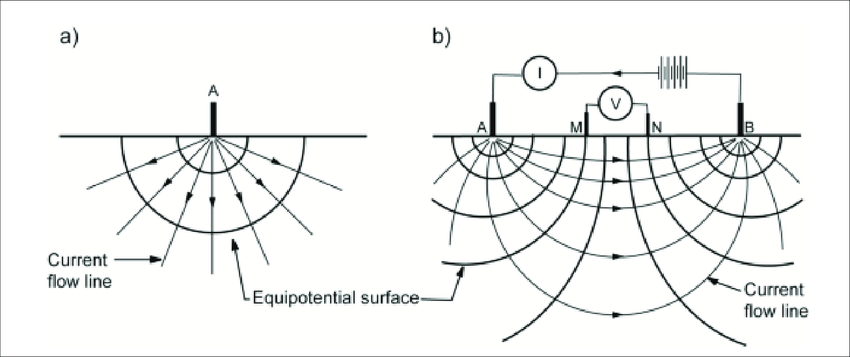
\includegraphics[width=0.95\textwidth]{Simplified-current-flow-lines-and-equipotential-surfaces-arising-from-a-a-single.png}
    \caption{Diagram illustrating electrical field with equipotential and current flow lines}
\end{figure}

\subsection{Apparent Resistivity}
Data from resistivity surveys are customarily presented and interpreted in the form of values of apparent resistivity \(\rho_a\). Apparent resistivity is defined as the resistivity of an electrically homogeneous and isotropic half-space that would yield the measured relationship between the applied current and the potential difference for a particular arrangement and spacing of electrodes. Wherever these measurements are made over a real heterogeneous earth, as distinguished from the fictitious homogeneous half-space, the symbol \(\rho\) is replaced by \(\rho_a\) for apparent resistivity.

Apparent resistivity is the bulk resistivity value obtained from field measurements. It is calculated using:
\begin{equation}
\rho_a = K \frac{\Delta V}{I}
\end{equation}

where:
\begin{itemize}
    \item $\rho_a$ = Apparent Resistivity ($\Omega m$),
    \item $\Delta V$ = Measured Potential Difference ($V$),
    \item $I$ = The Injected current ($A$).
\end{itemize}

Apparent resistivity is interpreted to estimate true resistivity, accounting for geological and geometric influences. Understanding apparent resistivity is crucial for interpreting field data and creating subsurface models.

\begin{figure}[h]
    \centering
    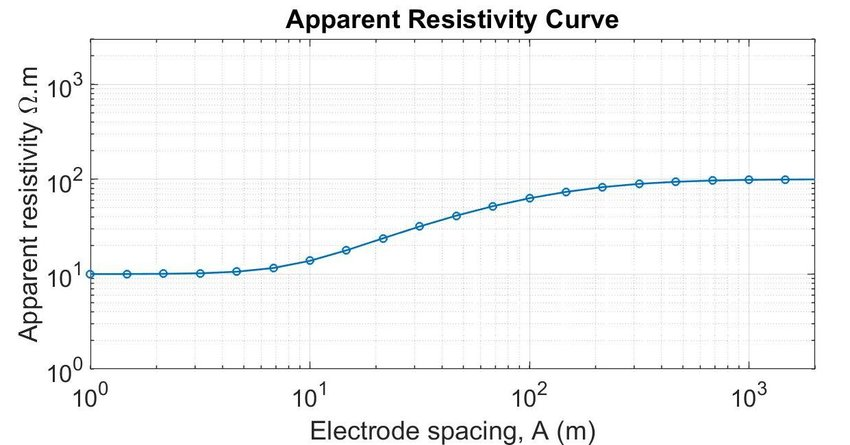
\includegraphics[width=0.95\textwidth]{Apparent-resistivity-curve-for-a-two-layer-model.png}
    \caption{Graph showing an apparent resistivity curve for a typical VES survey.}
\end{figure}

\subsection{The General Four Electrode System}

The four-electrode system is a standard configuration for resistivity surveys, comprising two current electrodes (A and B) and two potential electrodes (M and N). This setup minimizes contact resistance effects and ensures accurate measurements. The purpose is to measure the electrical resistivity of materials or earth layers by eliminating contact resistance between the electrodes and the material.

Consider an arrangement consisting of a pair of current electrodes and a pair of potential electrodes (Figure 3(a)). The current electrodes A and B act as source and sink, respectively. At the detection electrode C, the potential due to the source A is:

\begin{equation}
\phi_{C} = \frac{\rho I}{2\pi} \left( \frac{1}{r_{AC}} - \frac{1}{r_{CB}} \right)
\end{equation}

Similarly, the resultant potential at D is:

\begin{equation}
\phi_{D} = \frac{\rho I}{2\pi} \left( \frac{1}{r_{AD}} - \frac{1}{r_{DB}} \right)
\end{equation}

The potential difference measured by a voltmeter connected between C and D is:

\begin{equation}
\phi = \frac{\rho I}{2\pi} \left\{ \left( \frac{1}{r_{AC}} - \frac{1}{r_{CB}} \right) - \left( \frac{1}{r_{AD}} - \frac{1}{r_{DB}} \right) \right\}
\end{equation}

All quantities in this equation can be measured at the ground surface except the resistivity, which is given by:

\begin{equation}
\rho_a = 2\pi \frac{\phi}{I} \left\{ \frac{1}{\left( \frac{1}{r_{AC}} - \frac{1}{r_{CB}} \right) - \left( \frac{1}{r_{AD}} - \frac{1}{r_{DB}} \right)} \right\}
\end{equation}

This resistivity is known as apparent resistivity, which is equivalent to the true resistivity only when the latter is uniform throughout the subsurface. Otherwise, it must be looked upon as the most convenient way to represent the resistivity in the subsurface based on surface measurements. If the electrodes are laid out along a line and their separations are increased systematically, the change in apparent resistivity (as defined in Equation (6)) with electrode spacing makes it possible to determine the variation of resistivity with depth, within limits of precision that depend on the subsurface layering configuration.
\subsection{Electrode Configuration}
Electrode configuration (electrode array) A geometrical pattern of electrodes used in electrical sounding, constant-separation traversing, and induced polarization surveys. Usual configurations comprise two current electrodes and two potential electrodes whose separations are known and defined by a geometric factor. Common configurations include the Schlumberger arrays, Wenner arrays and dipole-dipole.

\subsubsection{Schlumberger Array:} 
Ideal for vertical profiling and depth estimation and commonly used in \textbf{Vertical Electrical Sounding (VES)} Surveying For this array, in the limit as \textit{a} approaches zero, the quantity V/a approaches the value of the potential gradient at the midpoint of the array.  In practice, the sensitivity of the instruments limits the ratio of s to a and usually keeps it within the limits of about 3 to 30.  Therefore, it is typical practice to use a finite electrode spacing. The apparent resistivity (r) is:

\begin{equation}
    \rho_a = \pi a \left[ \frac{s^2}{a} - \frac{a}{4} \right] \frac{V}{I} = \pi a \left[ \left( \frac{s}{a} \right)^2 - \frac{1}{4} \right] \frac{V}{I},
\end{equation}

\subsubsection{Wenner Array:}
This is suitable for horizontal profiling with uniform sensitivity and commonly used in \textbf{Constant Separation Traversing (CST)} Surveying. This array consists of four electrodes in line, separated by equal intervals, denoted a. After derivation, the user will find that the geometric factor K is equal to a , so the apparent resistivity is given by:

\begin{equation}
    \rho_a = \pi a \left[ \frac{s^2}{a} - \frac{a}{4} \right] \frac{V}{I} = \pi a \left[ \left( \frac{s}{a} \right)^2 - \frac{1}{4} \right] \frac{V}{I},
\end{equation}

\subsubsection{Dipole-Dipole Array:}
It provides high-resolution imaging for lateral changes. The dipole-dipole array is one member of a family of arrays using dipoles (closely spaced electrode pairs) to measure the curvature of the potential field.  If the separation between both pairs of electrodes is the same a, and the separation between the centers of the dipoles is restricted to a(n+1), the apparent resistivity is given by:

\begin{equation}
    \rho_a = \pi an (n + 1)(n + 2) \frac{V}{I},
\end{equation}

\begin{figure}[H]
    \centering
    \begin{subfigure}[t]{0.9\textwidth}
        \centering
        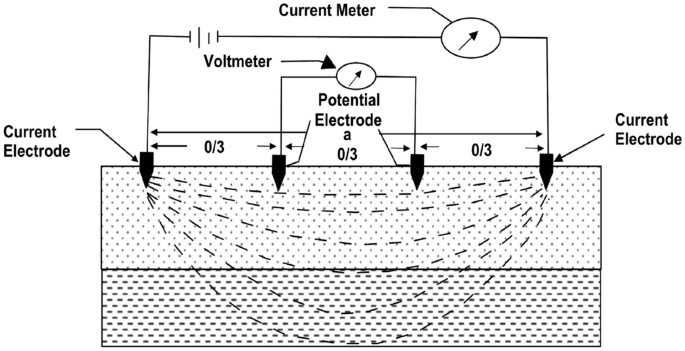
\includegraphics[height=0.3\textheight]{sclumberger.png}
        \caption{Schematic diagram of the Schlumberger array electrode configuration}
        \label{fig:schlumberger}
    \end{subfigure}\\[2cm]
    \vspace{1cm}
    \begin{subfigure}[t]{0.9\textwidth}
        \centering
        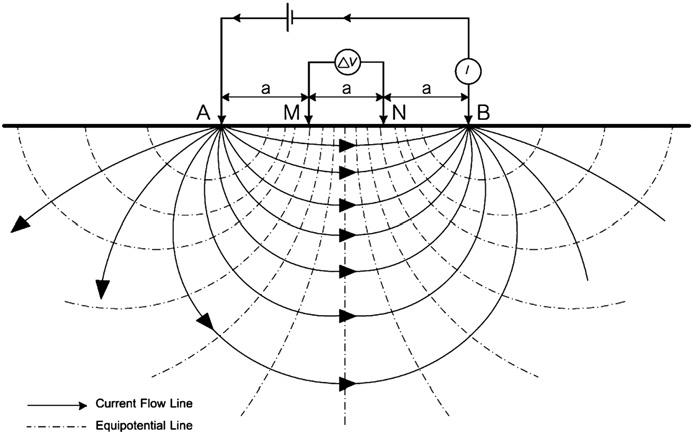
\includegraphics[height=0.35\textheight]{wenner.png}
        \caption{Schematic diagram of the Wenner array electrode configuration}
        \label{fig:wenner}
    \end{subfigure}
    \caption{Comparison of the Schlumberger and Wenner array electrode configurations.}
    \label{fig:configurations}
\end{figure}

\section{Resistivity Surveying Techniques}

\subsection{Resistivity Surveying}
Resistivity surveying is a geophysical method used to explore and characterize the subsurface by measuring the electrical properties of the ground. This technique is particularly valuable for mapping various geological features such as stratigraphy, fractures, faults, and groundwater zones. By injecting electrical current into the ground and measuring the resulting potential differences, resistivity surveying provides insights into the distribution of materials with different electrical resistivities beneath the Earth's surface. These measurements are crucial for a variety of applications including environmental studies, engineering projects, archaeological investigations, and hydrogeological assessments.

The principle behind resistivity surveying is based on the fact that different materials, like clay, sand, rock, or water, have distinct electrical resistivities. For instance, water-saturated zones typically have lower resistivity due to the conductive nature of dissolved salts, whereas dry, compact rocks might show higher resistivity. By interpreting these resistivity variations, geophysicists can infer the presence of different subsurface layers or structures.

\subsubsection{Steps for carrying out Resistivity Surveying:}
\begin{enumerate}
    \item \textbf{Planning the Survey:} Before setting up, a detailed plan is created considering the survey objectives, the area's geology, and any known subsurface features. This includes choosing the appropriate electrode configuration (like Wenner, Schlumberger, or Dipole-Dipole arrays) based on the depth and resolution required.

    \item \textbf{Set Up Electrodes Along the Survey Line:} Electrodes are strategically placed along a predetermined line or grid pattern. The spacing between electrodes can vary depending on the desired resolution and depth of investigation. For deep surveys, wider spacing might be used, while for shallow investigations, closer spacing is preferred.

    \item \textbf{Inject Current Using an External Source:} An external power source, typically a battery or generator, is used to inject a known current into the ground through two current electrodes. The choice of current magnitude is important as it should be sufficient to produce measurable potential differences without causing electrode polarization or overheating.

    \item \textbf{Measure Potential Differences at Specific Electrode Configurations:} Using two potential electrodes, the voltage difference resulting from the current flow is measured. This step is repeated at various configurations or along the survey line to gather comprehensive data. Modern resistivity meters automate this process, ensuring precision in measurements.

    \item \textbf{Calculate Apparent Resistivity and Analyze Results:} The apparent resistivity is calculated using formulas that incorporate the measured potential difference, the injected current, and the geometric factor of the electrode array. This apparent resistivity might not directly represent the true resistivity due to the complex nature of subsurface materials but provides a basis for interpretation. 
    \begin{itemize}
        \item \textit{Data Processing:} Collected data is processed to remove noise, correct for any systematic errors, and sometimes to transform the data into a more interpretable form like 2D or 3D resistivity models.
        \item \textit{Interpretation:} Geophysical software or manual interpretation methods are used to analyze the resistivity data. This step involves correlating resistivity values with known geological properties, which might require integration with other geophysical or geological data.
        \item \textit{Validation:} Often, the results are validated through drilling or other direct methods to confirm the presence of predicted features like aquifers or fault lines.
    \end{itemize}
\end{enumerate}

\subsection{Vertical Electrical Sounding}
The vertical electrical sounding or geoelectric method is one of the most used electrical geophysical techniques thanks to its simplicity and relative low cost. These are especially useful in hydrogeological studies where it is necessary to define and characterize deep phreatic levels. Vertical electrical sounding or SEV are a geophysical technique that, by means of electricity, allows recognizing or distinguishing the different geological formations that are found in depth and delimiting them. Electrical or electromagnetic geophysical techniques are based on measuring the resistivity of materials or conductivity.

Vertical Electrical Sounding (VES) is one-dimensional direct current electrical resistivity method, which consists of introducing a continuous electrical current of known intensity into the ground through two or more emitting electrodes, commonly called A and B, and measuring the electric potential difference using another pair of receiving electrodes, M and N, in this way it is possible to obtain the induced potential and the vertical distribution of the resistivities of the traversed formations. Using this method, the depth of study is directly proportional to the distance between the current electrodes and/or the potential electrodes used, so that the greater the separation distance between the electrodes, the greater the depth of the soil to be studied, while a spacing between the electrodes will measure the resistivity distribution in the subsurface at shallower depths. In this method, the results are compared with the common resistivities of the different materials, which allows them to be differentiated from each other.

The current injection electrodes A and B, and the potential measurement electrodes M and N, are arranged aligned in a certain structure, for this different configurations called “electrode device” are used, some of the most used are the Schlumberger configuration , Wenner and Dipole-Dipole.

\subsection{Constant Separation Traversing}
The object of electric horizontal profiling or combined Traversing
approach is to detect the lateral variations in the resistivity of the ground. In
Schlumberger method of electrical profiling, the current electrodes (AB)
remains fixed at a relatively large distance, for instance, a few hundred meters,
and the potential electrodes (MN) with a small constant separation \textbf{(Sharma
1986)}.

The appearance of the resistivity profile obtained by horizontal profiling will
depend not only on the positions of the potential electrodes M and N, but also
on the positions of the current electrodes A and B with respect to the
inhomogeneities in the earth and the reason behind that is that all electrodes are
moved after each measurement \textbf{(Kunetz, 1966)}.

The effect of vertical structures e.g. (faults, fissures, dikes, veins, and shear
zones) is lateral. If these features crop out, abrupt discontinuities in the slope of
\((\rho_a\)) curves are obtained as the mobile electrode configuration crosses the
vertical resistivity boundary. Many of key features found in the resistivity
anomalies over a vertical fault are found also in anomalies over near vertical
structures. The fault represents a vertical contact problem between two media of
differing resistivity. Therefore, the calculated curves for \((\rho_a\)) are discontinuous
at the vertical boundary. The discontinuity will be evident in practice as a steep
gradient in the resistivity curve \textbf{(Sharma, 1986)}.

The traversing obtained by moving an electrode spread with fixed electrode
separation along a traverse line, the array of electrodes being aligned either in
the direction of the traverse (longitudinal traverse) or at right angles to it
(transverse traverse). The former technique is more efficient as only a single
electrode has to be moved from one end of the spread to the other, and the
electrodes reconnected, between adjacent readings. The Vertical discontinuity
distorts the direction of current flow and thus the overall distribution of
potential in its vicinity.

\subsection{Comparison of VES and CST}

\begin{tabular}{|>{\raggedright\arraybackslash}m{4cm}|>{\raggedright\arraybackslash}m{6cm}|>{\raggedright\arraybackslash}m{6cm}|}
    \hline
    \textbf{Aspect} & \textbf{VES (Vertical Electrical Sounding)} & \textbf{CST (Constant Separation Traversing)} \\ \hline
    
    \textbf{Application} & Used for determining vertical variations in subsurface resistivity, often for geological or hydrological studies. & Used for mapping horizontal variations in subsurface resistivity over a specific area. \\ \hline
    
    \textbf{Field Survey} & Involves inserting electrodes into the ground at different depths along a vertical profile to measure resistivity changes with depth. & Electrodes are placed at a constant separation, and measurements are taken as the array is moved horizontally across the survey area. \\ \hline
    
    \textbf{Cost} & Costs include equipment, labor for setting up electrodes at various depths, and data analysis. & Similar costs but potentially less labor-intensive as electrode setup is simpler with fixed separation. \\ \hline
    
    \textbf{Formula} & Resistivity is calculated using formulas like $\rho_a = \pi a \left[ \frac{s^2}{a} - \frac{a}{4} \right] \frac{V}{I}$. & Similar resistivity formulas but applied in a horizontal context, often using a Wenner or Schlumberger array configuration. \\ \hline
    
    \textbf{Purpose} & To provide a vertical profile of resistivity, useful for identifying depth to bedrock, water table, or different soil layers. & To provide a horizontal map of resistivity, useful for detecting lateral changes like faults, buried structures, or contaminant plumes. \\ \hline
    
    \textbf{Advantages} & Offers detailed information on vertical resistivity changes, which can be critical for depth-specific investigations. & Efficient for covering large areas to identify lateral resistivity variations, providing a broader spatial understanding. \\ \hline
    
    \textbf{Challenges} & Requires precise depth control and can be influenced by surface conditions; time-consuming for deep profiling. & Less detailed in vertical resolution, and lateral resolution depends on electrode spacing; can be affected by surface irregularities. \\ \hline
\end{tabular}

\section{Previous Studies on Electrical Resistivity}

\subsection{Historical Context and Key Findings}
Electrical resistivity methods have evolved over the decades, with significant advancements in equipment and interpretation techniques. Early studies laid the groundwork for modern applications in groundwater exploration, mining, and foundation design. Previous studies have demonstrated the effectiveness of electrical resistivity in identifying subsurface anomalies such as fractures, cavities, and weak zones. These findings are crucial for designing safe and durable foundations.

\subsection{Previous Studies in Nigeria}

Several authors have contributed to the application of electrical resistivity methods in civil engineering investigations. \textbf{Akintoye \textit{et al.,} (2018)} investigated the subsurface conditions of an unstable slope in southwestern Nigeria using the electrical resistivity method. The study employed the Schlumberger configuration to delineate weak zones and fractures, revealing that high resistivity anomalies correspond to compact lithological units, while low resistivity zones indicate water-saturated regions. The results were used to recommend appropriate foundation designs for slope stabilization. \textbf{Adeyemi and Bello (2020)} conducted a geophysical evaluation of construction sites in Lagos, Nigeria, to identify potential risks associated with heterogeneous subsurface layers. Using Vertical Electrical Sounding (VES), the authors mapped lithological variations and identified zones of high porosity and low bearing capacity. The findings highlighted the importance of resistivity surveys in mitigating structural failures. \textbf{Olayemi \textit{et al.,} (2021)} applied electrical resistivity tomography (ERT) to assess subsurface integrity for a proposed bridge site. The study identified a highly fractured zone beneath the surface, which could pose a risk to structural stability. The authors recommended relocating the foundation to a more stable area, emphasizing the reliability of ERT in civil engineering applications. \textbf{James and Olatunji (2019)} focused on the use of geophysics for groundwater exploration in arid regions. Though primarily aimed at water resource management, their work demonstrated the potential of resistivity methods in identifying zones with sufficient bearing capacity for construction purposes.

\subsection{Comparison of Methods}
Various configurations have been used in resistivity surveys, including Schlumberger, Wenner, and Dipole-Dipole arrays. \textbf{(Eze \textit{et al.,} 2017)} compared these methods for subsurface investigations and found that the Schlumberger array is more effective for deep-layer detection, while the Wenner array provides better horizontal resolution. Their research underscores the need to select an appropriate configuration based on site-specific requirements. \textbf{(Telford \textit{et al.,} 1990)} further elaborated on the principles of resistivity methods, offering insights into how the Wenner array can be adapted for high-resolution near-surface investigations. Their book, \textit{Applied Geophysics}, is a seminal text that discusses various resistivity techniques and provides a detailed analysis of their applications in subsurface investigations. The authors emphasized that while the Schlumberger configuration excels in depth penetration, the Wenner method remains superior for detailed mapping of near-surface anomalies.

\textbf{(Reynolds 2011)} provides a comprehensive guide on geophysical methods used in engineering, including electrical resistivity. In his book \textit{An Introduction to Applied and Environmental Geophysics}, he discusses how resistivity surveys are instrumental in civil engineering projects, especially in urban areas where the variability of subsurface properties poses significant challenges.
\section{Applications of Electrical Resistivity}

\subsection{Innovative Applications of Electrical Resistivity}
In recent years, there has been an increasing application of electrical resistivity methods in more complex subsurface investigations. \textbf{Steeples and Chilton (2001)} focused on the use of resistivity in mapping groundwater contamination in urban areas. They highlighted how advanced electrical resistivity tomography (ERT) can help locate pollution plumes in aquifers, enabling more efficient management of groundwater resources. Their work, published in \textit{Environmental and Engineering Geophysics}, underscores the growing versatility of resistivity methods in addressing both environmental and engineering concerns.

\textbf{Loke (2016)} provides a detailed exploration of the technological advancements in resistivity methods. In his book, \textit{Geoelectrical Imaging for Environmental and Engineering Applications}, he describes new developments in data acquisition systems, such as multi-electrode arrays, that have made resistivity surveys faster and more accurate. This book serves as a crucial resource for understanding the technical evolution of electrical resistivity methods and their broader application in modern engineering and environmental investigations.

\subsection{Applications in Structural Health Monitoring}
Electrical resistivity methods have also been explored for monitoring the health of structures over time. \textbf{Bermúdez \textit{et al.,} (2020)} demonstrated how electrical resistivity tomography can be employed to monitor the condition of reinforced concrete structures, detecting early signs of deterioration such as corrosion. Their study published in the \textit{Journal of Applied Geophysics} showed how resistivity surveys could be used for the non-destructive testing of infrastructure, offering a sustainable and cost-effective alternative to traditional inspection methods.
\textbf{Caldwell and Brown (2020)} conducted a study on the application of resistivity imaging for the monitoring of railway tracks. Their work showed that electrical resistivity could be used to detect subtle shifts in the ground around the tracks, which could indicate potential risks like landslides or subsidence. Their findings, published in the \textit{Geophysical Journal International}, suggest that resistivity surveys can play a critical role in maintaining the integrity of transport infrastructure, especially in areas prone to natural disasters.

\subsection{Applications in Building Foundation}
\textbf{Falae (2014)} carried out a geophysical survey using Vertical Electrical Sounding (VES) at Ibese Southwestern Nigeria in his book published in the \textit{Asia Pacific Journal of Energy and Environment, Volume 1, No 2 (2014)} to determine the geophysical parameters that can be used to evaluate the structural competence of the subsurface geological characteristics of the site for construction purposes and building development. The Schlumberger configuration was used for the data acquisition. One-dimensional numerical inversion of individual DC resistivity was used to enhance the processing of the results for better achievement of the aim of the study. Models obtained from the 2D inversion of each VES were used for construction of geo-electric sections which exhibit the main geo-electric characteristics of the geological units present in the area. 

\section{Importance of Subsurface Evaluation for Foundation Design}

Subsurface evaluation is a critical aspect of civil engineering, particularly in foundation design, as the stability, safety, and longevity of structures heavily depend on the underlying ground conditions. Inadequate knowledge of subsurface characteristics often leads to construction challenges, foundation failures, and increased project costs.

\subsection{Understanding Subsurface Conditions:}
The subsurface environment is inherently heterogeneous, comprising varying soil types, rock layers, and groundwater conditions. Evaluating these factors provides insights into:

\begin{itemize}
    \item \textbf{Soil Properties:} Characteristics such as density, cohesion, and angle of internal friction influence a soil's load-bearing capacity and compressibility.
    \item \textbf{Rock Layers:} The depth and quality of bedrock can affect the choice of foundation type and its depth.
    \item \textbf{Groundwater Table:} The presence of groundwater impacts soil strength and stability, making its identification crucial for waterproofing and structural integrity.
\end{itemize}

\subsection{Benefits of Subsurface Evaluation:}
\begin{itemize}
    \item \textbf{Foundation Stability:} Subsurface evaluation ensures that the chosen foundation type is compatible with site-specific conditions, reducing the risk of settlement or failure.
    \item \textbf{Cost Efficiency:} Early identification of subsurface issues prevents unforeseen complications during construction, minimizing delays and cost overruns.
    \item \textbf{Environmental Safety:} Identifying geological hazards such as faults or contaminated soils mitigates risks to the structure and surrounding environment.
    \item \textbf{Design Optimization:} Provides engineers with critical data for designing efficient and durable foundations tailored to site-specific conditions.
\end{itemize}

\subsection{Case Studies in Foundation Design:}
Several studies have demonstrated the importance of subsurface evaluation including \textbf{Akintoye \textit{et al.,} (2018)} used seismic refraction to detect weak zones in an unstable slope, enabling optimized foundation design for slope stabilization. \textbf{Adeyemi and Bello (2020)} applied Vertical Electrical Sounding (VES) to map lithological variations in Lagos, Nigeria, identifying zones of low bearing capacity and mitigating risks of structural failure. \textbf{Olayemi \textit{et al.,} (2021)} employed electrical resistivity tomography (ERT) to identify a fractured zone beneath a proposed bridge site, leading to the relocation of the foundation for safety.


\subsection{Relevance to Sustainable Construction:}
Subsurface evaluation aligns with sustainable construction practices by:
\begin{itemize}
    \item Minimizing material wastage through accurate design.
    \item Reducing the environmental impact of construction failures.
    \item Enhancing the resilience of structures against natural hazards.
\end{itemize}

\chapter{CHAPTER 3: MATERIALS AND METHODS}

\section{Introduction}
This chapter outlines the materials, equipment, and methodologies employed in the geophysical evaluation of subsurface layers for civil engineering foundation design using electrical resistivity methods. The methods described here focus on Vertical Electrical Sounding (VES) and Constant Separation Traversing (CST), which were selected for their effectiveness in capturing vertical and lateral variations in subsurface resistivity. This chapter also discusses survey design, data acquisition, processing, interpretation, precautions, and limitations encountered during the study.

\section{Geophysical Survey Materials and Equipment}
The success of a geophysical survey depends on the appropriate selection and utilization of specialized materials and equipment. The following tools were employed:

\begin{itemize}
    \item \textbf{Resistivity Meter:} The core device used to inject current into the ground and measure the resulting potential difference. A digital resistivity meter (e.g., ABEM Terrameter) shown in fig 3.1 was utilized for precise and reliable measurements.
    \item \textbf{Steel Metal Electrodes:} Used as current and potential electrodes for injecting current into the ground and measuring potential differences. Electrodes were securely inserted into the soil to ensure good contact.
    \item \textbf{Connecting Wire Cables:} Insulated cables connected the resistivity meter to the electrodes, ensuring stable current flow and accurate measurements.
    \item \textbf{Measuring Tape:} Used to measure and maintain accurate spacing between electrodes according to the selected configuration.
    \item \textbf{Hammer:} Assisted in driving electrodes into hard or compact ground surfaces.
    \item \textbf{Clips:} Metal clips were used to secure the cables to the electrodes and maintain strong connections.
    \item \textbf{Compass:} Used to align survey lines and ensure consistent electrode orientation relative to the site layout.
    \item \textbf{Global Positioning System (GPS):} Employed to accurately record the geographical coordinates of each survey station.
    \item \textbf{Data Recording Materials:} Included field notebooks, data sheets, and digital storage devices for logging measurements and observations.
\end{itemize}
    
\begin{figure}[h]
    \centering
    \includegraphics[width=0.70\textwidth]{IMG_9200.jpg}
    \caption{The Resistivity Meter used for the Survey.}
\end{figure}

\section{Methodology}
\subsection{Survey Design}
\begin{itemize}
    \item \textbf{Selection of Electrode Configurations:}  
    Two configurations were selected to address different investigation goals:
    \subsubsection{- Schlumberger Configuration:} This configuration was chosen for VES due to its ability to penetrate deeper into the subsurface by gradually increasing the current electrode spacing. It provides detailed depth-specific resistivity data and is cost-effective for deep investigations.
    \subsubsection{- Wenner Configuration:} This configuration was employed for CST as it is sensitive to lateral variations in resistivity, making it ideal for detecting horizontal changes in subsurface layers. Its simplicity in setup allows for rapid data acquisition over large areas.
    \\[1cm]
    \begin{figure}[h]
        \centering
        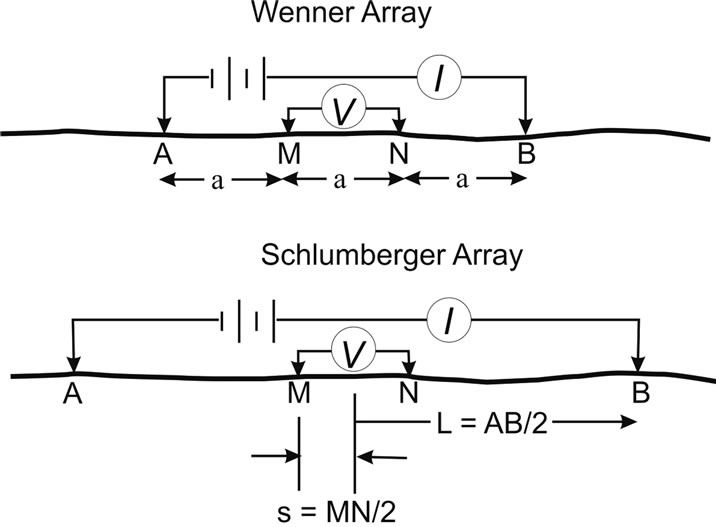
\includegraphics[width=0.85\textwidth]{wenner_schlum.jpg}
        \caption{Electrode Arrangement of Wenner and Schlumberger Configuration}
    \end{figure}

    \item \textbf{Survey Layout:}  
    The study area was systematically covered with 3 parallel profiles at first study area and 2 parallel profiles at second second study area, denoted as Profile 1 (130m), Profile 2 (150m) and Profile 3 (130m) at first study area, and  Profile 1 (130 m) and Profile 2 (150 m) at second study area, spaced apart to ensure adequate coverage. Profile endpoints and starting points are clearly marked, ensuring proper alignment during the survey. The profiles were oriented to maximize data collection over the expected subsurface structures, as informed by the geological context of the area. The survey also incorporated Vertical Electrical Sounding (VES) points, numbered VES1 to VES10 for each study area, which are distributed across the area for localized subsurface investigations. GPS was used to precisely locate the electrode positions, ensuring consistency and repeatability of the survey. Additionally, a grid-like "Box Layer" is superimposed over the study area for spatial referencing and visualization of the coverage.
    
    Here is the attached figure showing the survey layout for both study areas:
    
    \begin{figure}[H]
        \centering
        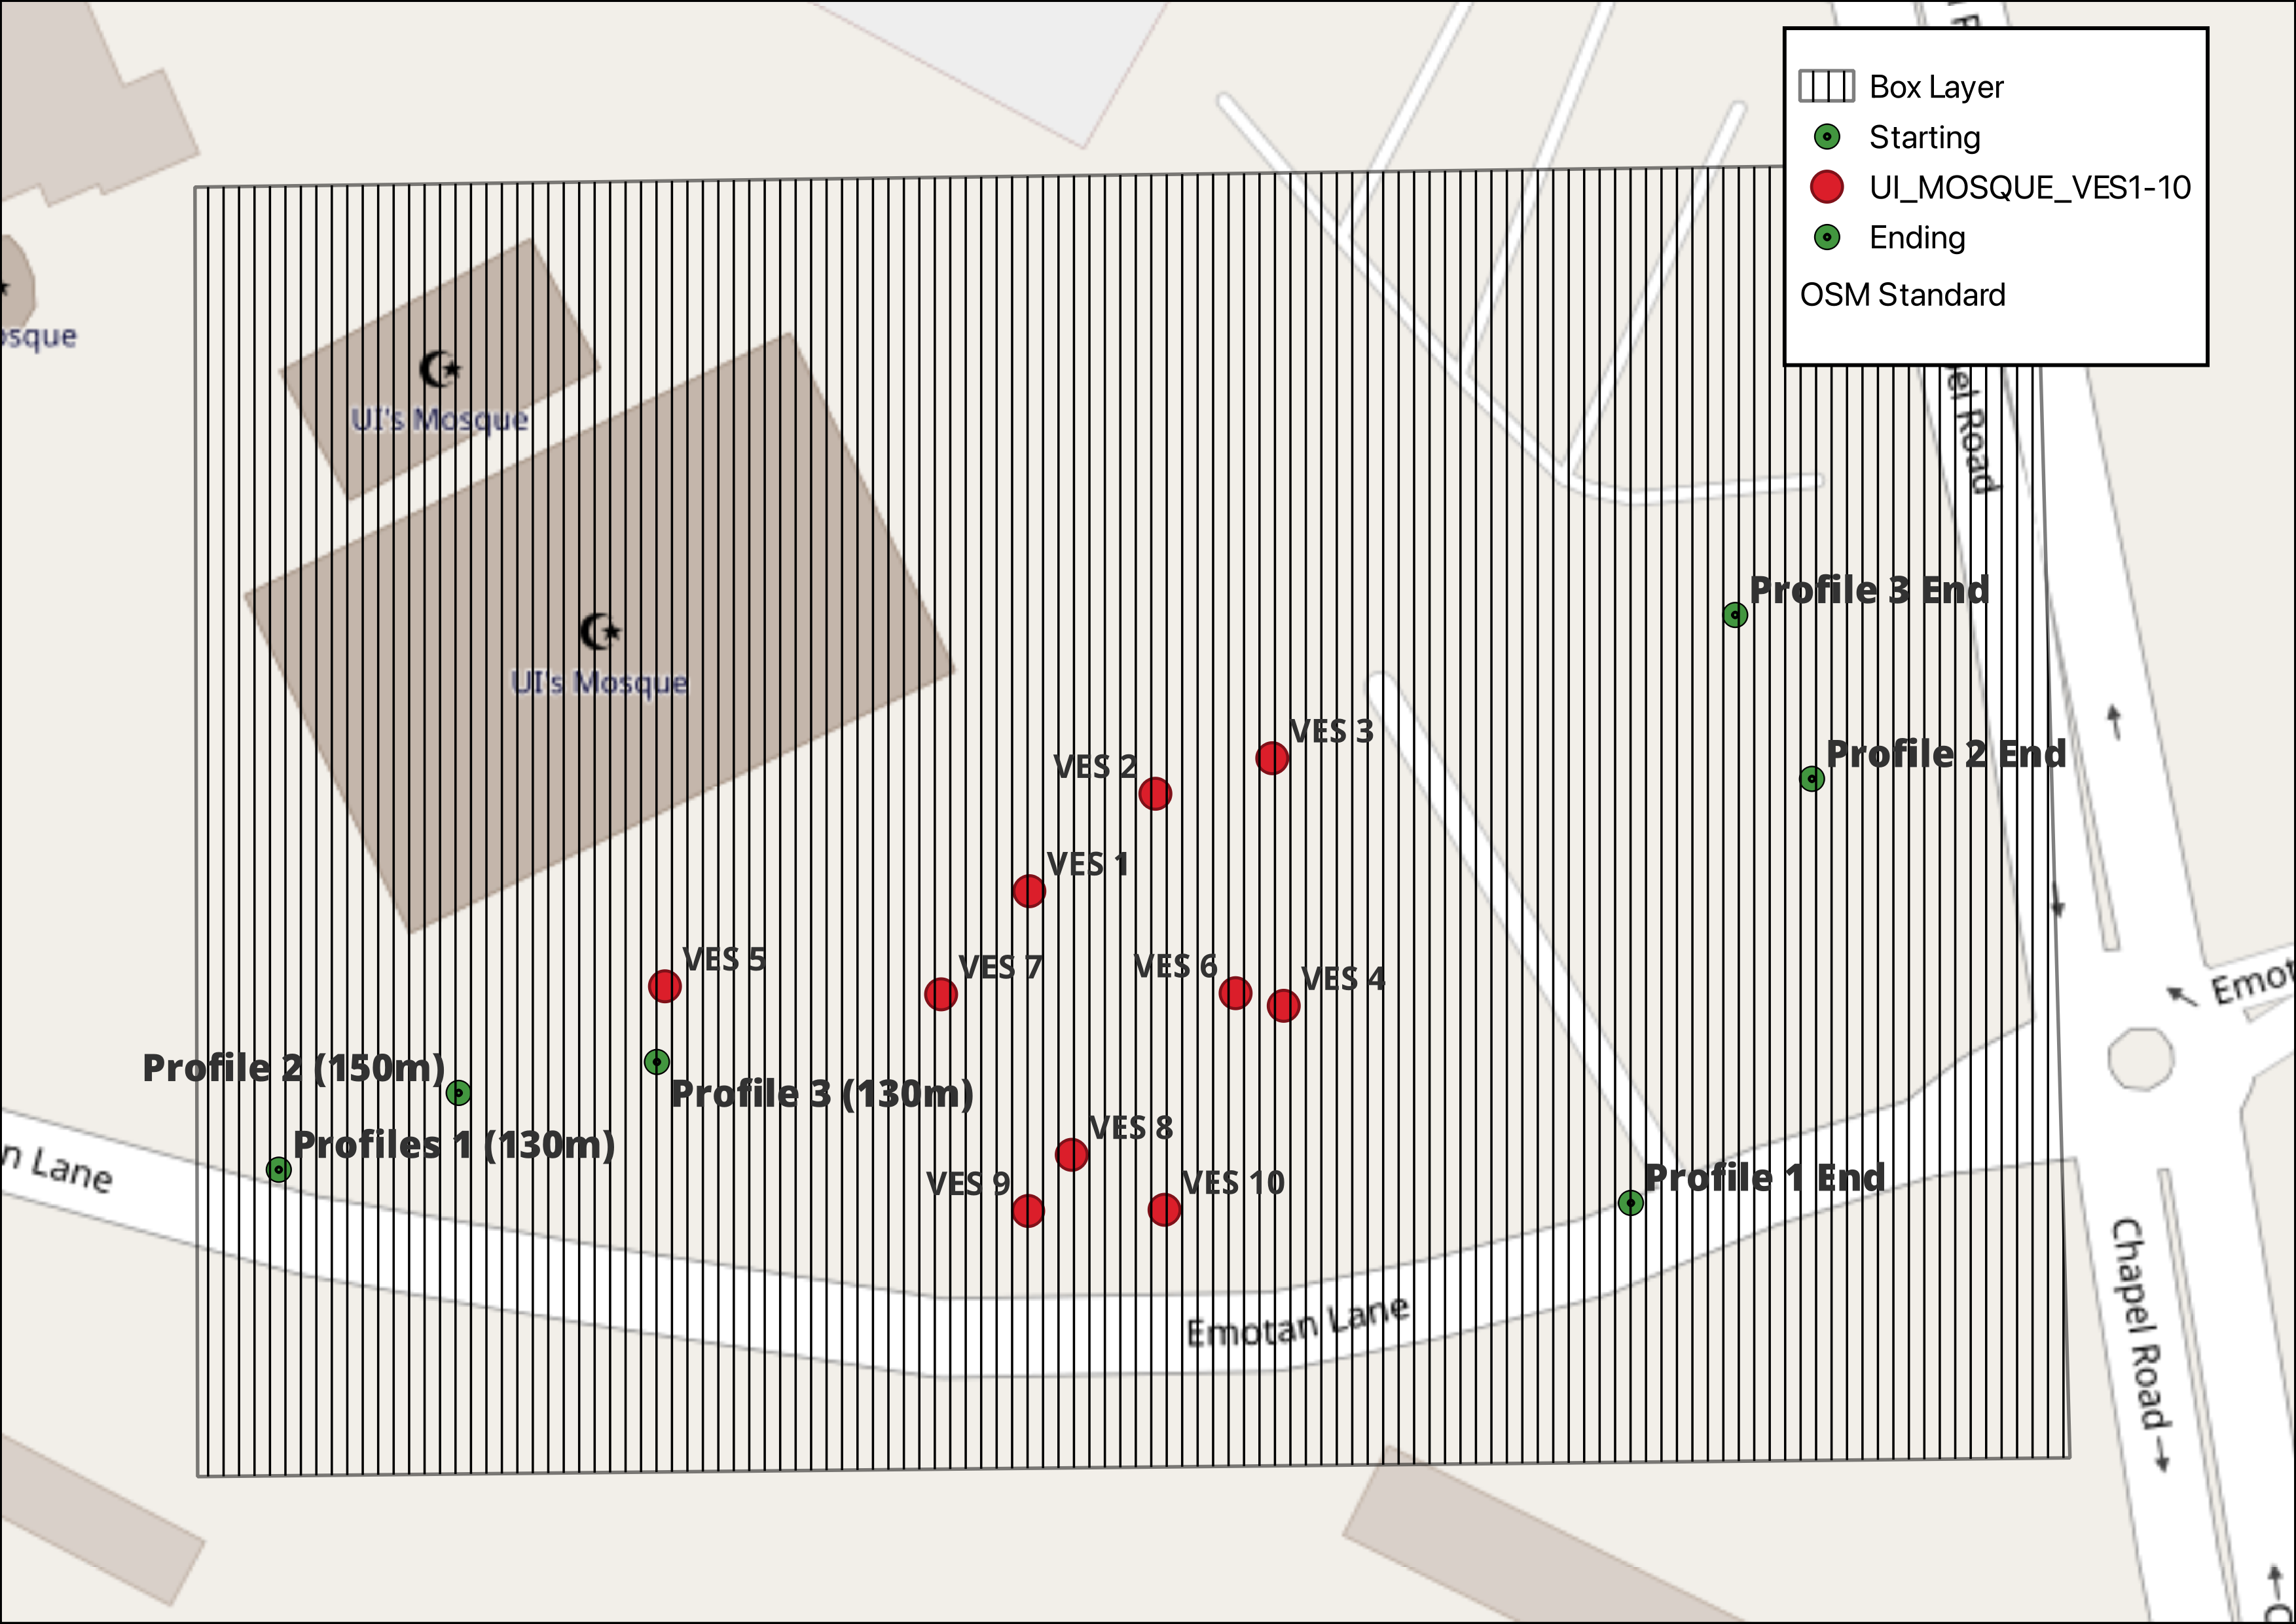
\includegraphics[width=0.85\textwidth]{Mosque_Survey_Layout.png}
        \caption{Survey Layout for UI Mosque Study Area}
        \label{fig:UI Mosque Survey Layout}
    \end{figure}

    \begin{figure}[H]
        \centering
        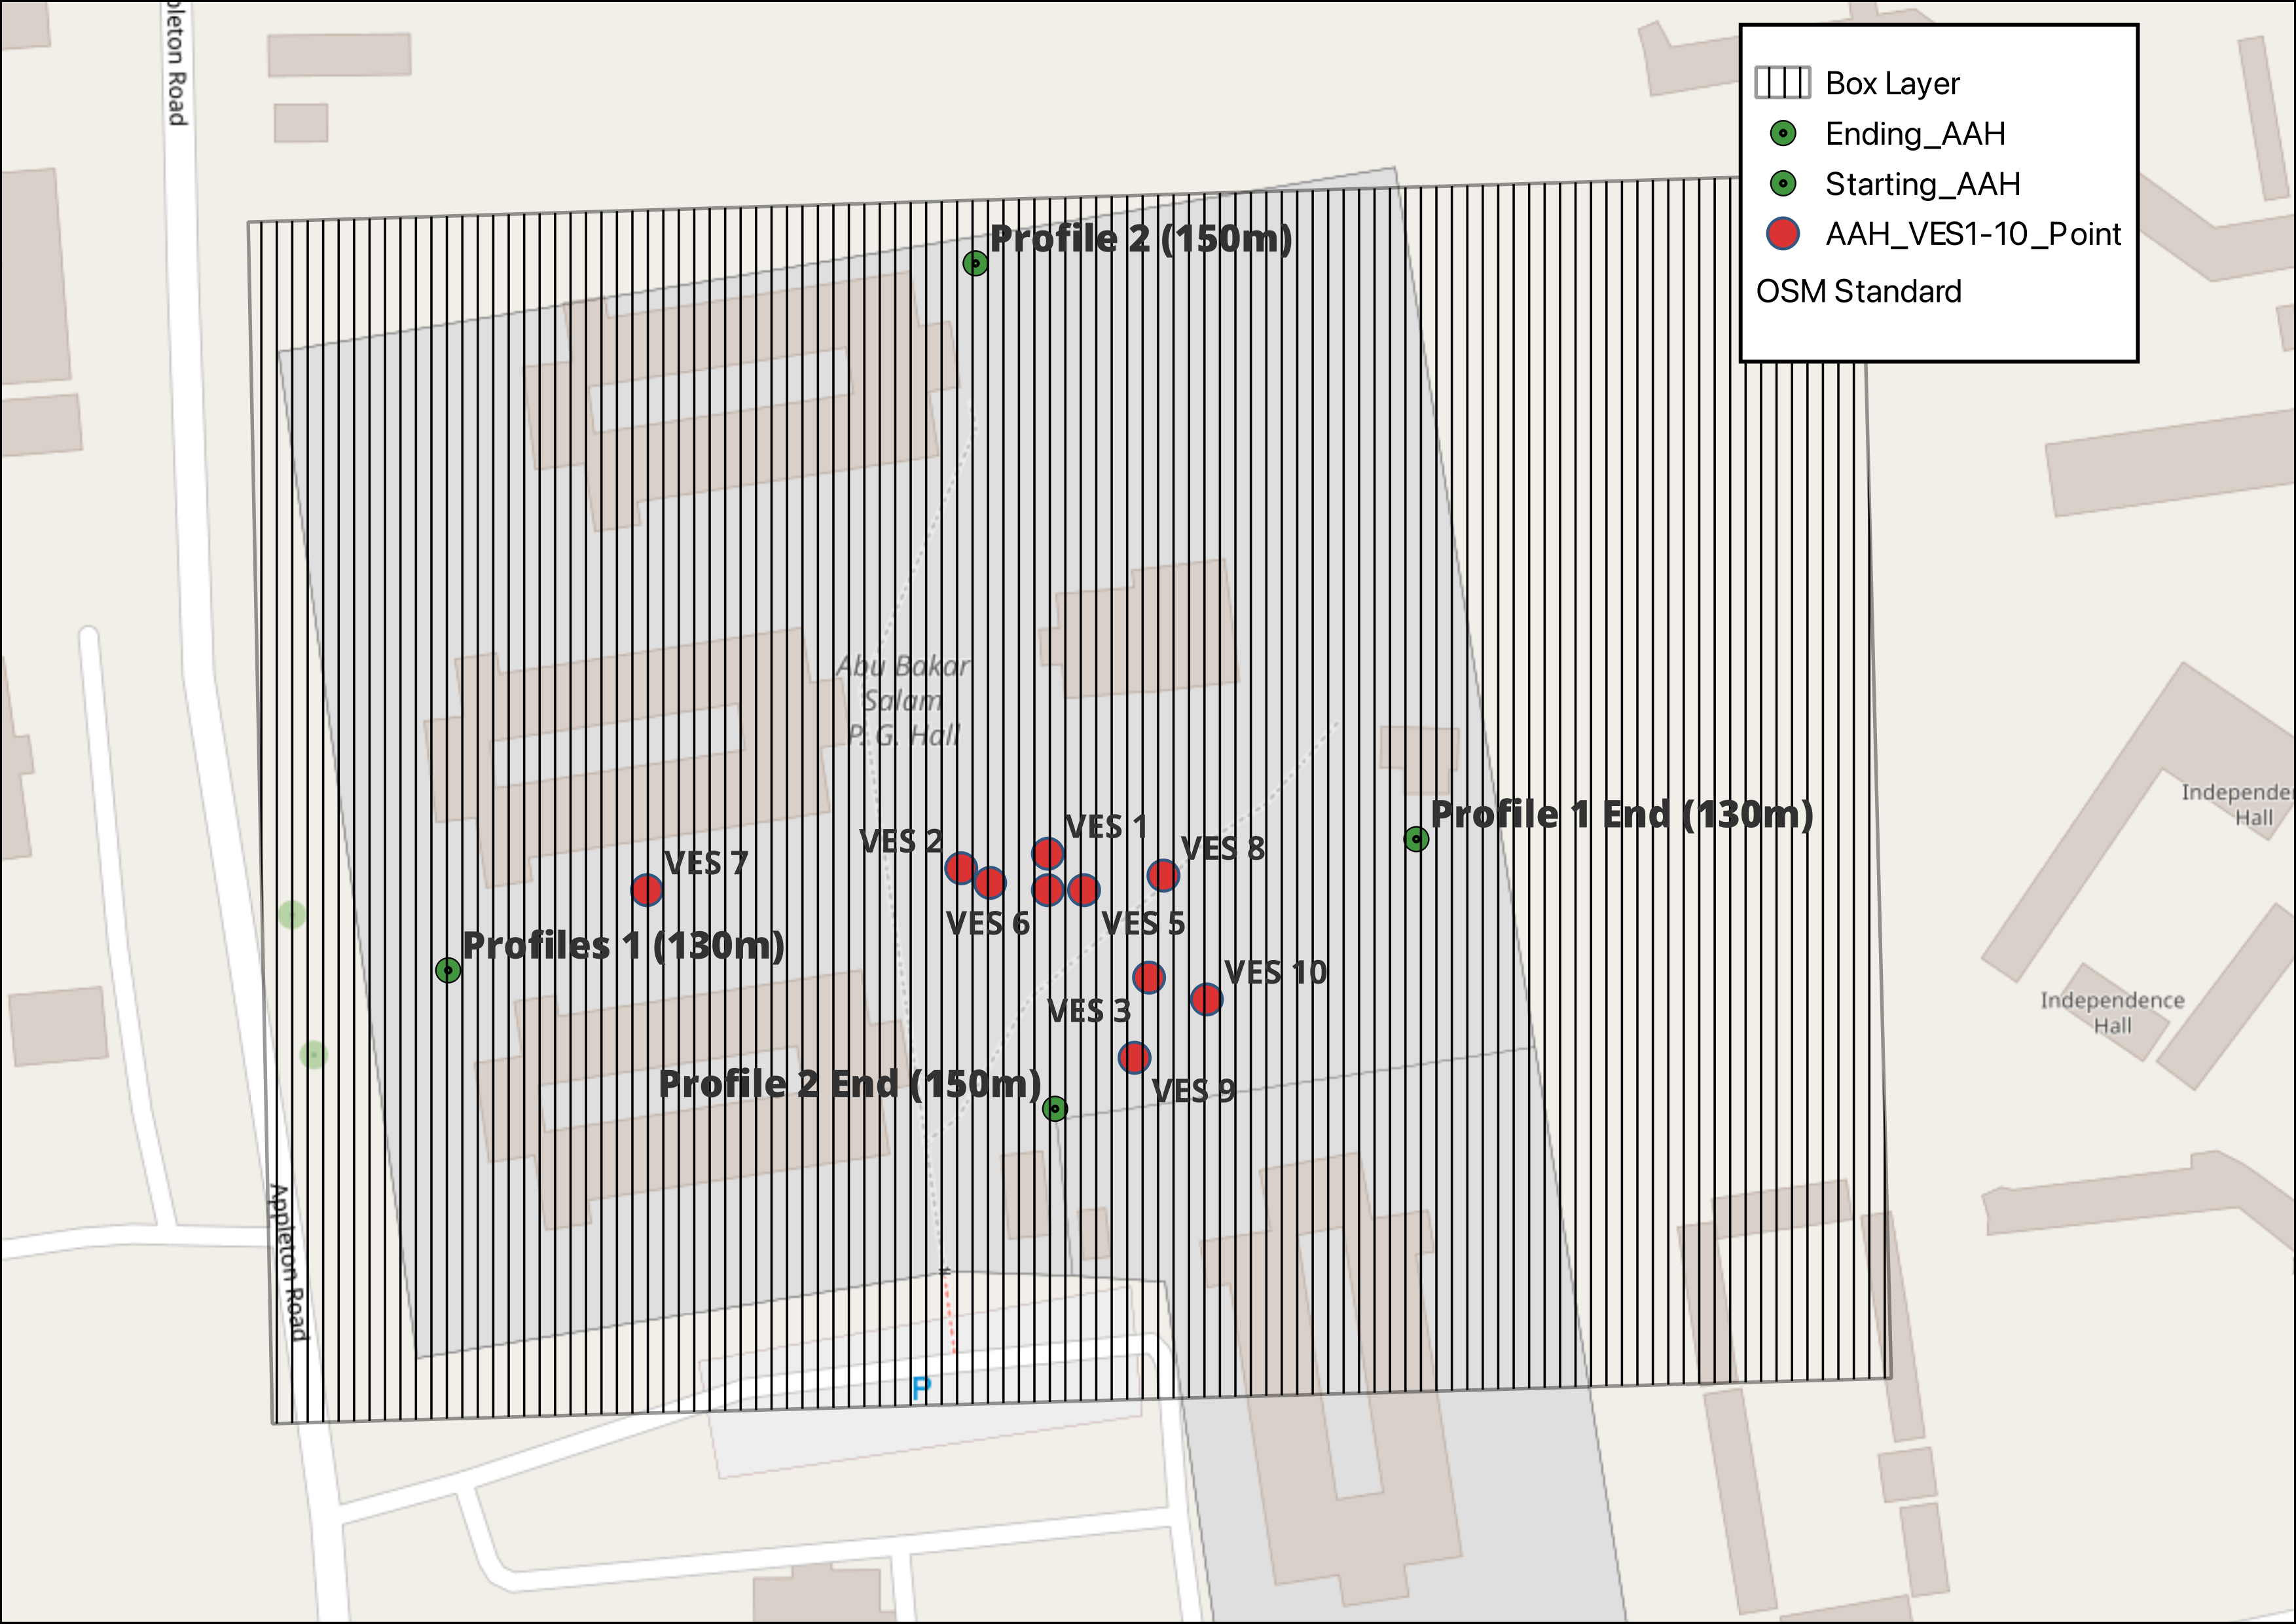
\includegraphics[width=0.85\textwidth]{AAH_Survery-Layout.png}
        \caption{Survey Layout for AAH Study Area}
        \label{fig:AAH Survey Layout}
    \end{figure}

\end{itemize}

\subsection{Field Procedures}
\begin{itemize}
    \item \textbf{Electrode Placement:} Electrodes were inserted into the ground at specified intervals based on the chosen configuration. Care was taken to ensure firm contact with the soil, especially in dry or compacted areas.
    \begin{figure}[H]
        \centering
        \includegraphics[width=0.7\textwidth]{IMG_9183.jpg}
        \caption{An Electrode Injected to the Ground }
    \end{figure}
    \item \textbf{Current Injection and Measurement:} A steady electrical current was injected into the ground through the outer electrodes. The potential difference was measured across the inner electrodes using the resistivity meter. Environmental factors such as moisture levels and soil conductivity were monitored to optimize measurements.
\end{itemize}

\subsection{Data Acquisition}
\begin{enumerate}
    \item \subsubsection{Vertical Electrical Sounding Data Acquisition}
    Data was collected at fixed points and the coordinates were recorded along the survey line by gradually increasing the spacing between current electrodes. The resulting apparent resistivity values were plotted against electrode spacing to generate depth profiles.
    \item \subsubsection{Constant Separation Traversing Data Acquisition}
    The electrode array was moved laterally along the survey lines with a fixed electrode spacing. Here the starting coordinates and the ending coordinates were recoreded and apparent resistivity values were recorded at regular intervals to map horizontal variations in subsurface resistivity.
\end{enumerate}

\subsection{Data Processing}
\begin{itemize}
    \item \textbf{Software Used:} The data was processed using software such as WINRESIST to get 1D with VES data for 2D and 3D resistivity modeling. DIPROWIN software was employed for contour plotting and visualization with CST data.
    \item \textbf{Data Correction:} Corrections were applied to remove noise caused by electrode polarization, environmental factors, or measurement errors. Calibration checks were performed to ensure the reliability of the resistivity meter.
    \item \textbf{Inversion Techniques:} The apparent resistivity values were inverted to obtain true resistivity, using iterative algorithms to refine the models. The final output included detailed resistivity profiles and maps.
\end{itemize}

\subsection{Interpretation Methods}
\begin{itemize}
    \item \textbf{Resistivity Models:} The processed data was used to construct 2D and 3D models of subsurface resistivity. These models highlighted lithological layers, groundwater zones, and potential weak zones.
    \item \textbf{Correlation with Geological Data:} Resistivity results were correlated with known geological features in the study area, including borehole logs and previous studies.
    \item \textbf{Validation:} Validation of the results was achieved by comparing the interpreted data with existing geological maps and, where available, borehole data.
\end{itemize}

\section{Limitations and Precautions}

\subsection{Limitations}
Electrical resistivity methods (ERM) are widely used for subsurface investigations, but they are not without limitations. These limitations can arise from environmental factors, methodological constraints, and inherent characteristics of the subsurface. Some of the key limitations include:

\begin{itemize}
    \item \textbf{Sensitivity to Noise:} ERM is highly sensitive to noise from external sources such as power lines, stray currents, and metallic objects in the survey area. These factors can distort measurements and affect data quality.
    \item \textbf{Limited Depth Penetration:} The depth of investigation is constrained by the maximum spacing of current electrodes. For deeper investigations, larger electrode spacing is required, which may not be feasible in restricted spaces or urban environments \textbf{(Binley, 2015)}.
    \item \textbf{Ambiguity in Interpretation:} Resistivity results are inherently non-unique, meaning that different subsurface conditions can produce similar resistivity patterns. This can lead to misinterpretation if additional validation methods, such as borehole logs, are not used \textbf{(Reynolds, 2011)}.
    \item \textbf{Effect of Geological Complexity:} In areas with highly heterogeneous geology, such as fractured zones or mixed lithologies, interpreting resistivity data can be challenging due to overlapping resistivity values \textbf{(Olayemi \textit{et al.,} 2021)}.
    \item \textbf{Dependence on Soil Moisture:} The resistivity of subsurface materials is strongly influenced by moisture content. Seasonal variations in soil moisture can lead to inconsistent results if surveys are conducted at different times of the year \textbf{(Farinde \textit{et al.,} 2015)}.
    \item \textbf{Environmental Impact:} In some cases, the insertion of electrodes can disturb the soil or vegetation. This is particularly a concern in sensitive ecological areas or agricultural lands.
    \item \textbf{Equipment Limitations:} The accuracy of resistivity measurements is dependent on the quality and calibration of the equipment used. Older or poorly maintained instruments can produce unreliable results.
    \item \textbf{Time and Labor Intensive:} Setting up electrodes and conducting surveys over large areas can be time-consuming, especially in rough terrains or areas with accessibility issues.
\end{itemize}

\subsection{Precautions}
To minimize the limitations of electrical resistivity methods and ensure reliable results, the following precautions should be taken:

\begin{enumerate}
    \item \textbf{Ensure Proper Electrode Contact:} Electrodes should be securely inserted into the ground to achieve good electrical contact. In dry or rocky areas, water or conductive gel can be used to improve contact.
    \item \textbf{Avoid Areas with High Noise Levels:} Surveys should be conducted away from power lines, pipelines, and other sources of electrical interference. If unavoidable, filters should be used to remove noise from the data.
    \item \textbf{Conduct Surveys During Stable Weather Conditions:} Avoid conducting surveys during extreme weather conditions, such as heavy rains or droughts, as these can affect soil resistivity and distort results.
    \item \textbf{Perform Regular Equipment Calibration:} The resistivity meter and other instruments should be calibrated before use to ensure accurate measurements. Regular maintenance is essential to avoid equipment malfunction.
    \item \textbf{Validate Results with Additional Methods:} To reduce ambiguity, resistivity results should be validated using borehole data, geological maps, or other geophysical methods like seismic or ground-penetrating radar \textbf{(Reynolds, 2011)}.
    \item \textbf{Use Appropriate Electrode Configurations:} Select the electrode configuration (e.g., Schlumberger or Wenner) that best suits the survey objectives and site conditions. This ensures optimal resolution and depth coverage.
    \item \textbf{Minimize Environmental Impact:} Take measures to reduce soil and vegetation disturbance when placing electrodes, especially in environmentally sensitive areas.
    \item \textbf{Plan for Accessibility:} In areas with difficult terrain or limited access, plan the survey layout in advance to ensure all necessary locations can be reached without compromising data quality.
    \item \textbf{Conduct Pre-Survey Reconnaissance:} Assess the site for potential obstacles, such as rocks, buried utilities, or water bodies, that may interfere with the survey.
    \item \textbf{Record Detailed Field Notes:} Document all field conditions, instrument settings, and environmental factors during the survey. This information is crucial for data interpretation and troubleshooting.
\end{enumerate}

\chapter{CHAPTER 4: RESULTS AND ANALYSIS}

\section{Introduction}
\justifying
This chapter presents a comprehensive overview of the results obtained from the geophysical surveys conducted at two distinct study areas: Emotan Lane near the University of Ibadan Central Mosque, and Appleton Road in Abubakar Abdulsalam Hall within the University of Ibadan campus. These results are analyzed and interpreted to understand the subsurface resistivity variations, geological features, and structural anomalies, including subsurface layers, faults, and other resistivity contrasts. The data acquisition processes utilized both Vertical Electrical Sounding (VES) and Constant Separation Traversing (CST) techniques, employing the Schlumberger and Wenner array configurations, respectively. These methods were chosen for their reliability and effectiveness in delineating subsurface structures and identifying resistivity anomalies.

The interpretation of field data involved practical curve matching techniques and computer-assisted analysis using WINRESIST and DIPROWIN software, which facilitated the generation of layered models and resistivity profiles. Additionally, Surfer software was used to create contour maps and visualize subsurface variations along the established profiles. This chapter also provide insights into the resistivity characteristics of the basement complex and their implications for understanding the structural integrity, fault systems, and other geophysical anomalies in the study areas. The findings are presented in the form of tables, graphs, and contour maps to enhance clarity and support the discussions.

\section{Data Acquisition and Study Areas}
A total of 20 VES stations were recorded, with 10 stations in each study area. Additionally, three CST profiles were conducted at the first location, and two CST profiles were carried out at the second location. The tables below present the data obtained from the fieldwork.

\subsection{Vertical Electrical Sounding Resistivity Field Records}
\textbf{Location:} {Emotan Lane, University of Ibadan Central Mosque, Ibadan.} \\
\textbf{Instrument:} {Campus Omega Resistivity Meter} \\
\textbf{Array Type:} {Schlumberger Array }

\begin{table}[h!]
    \centering
    \begin{adjustbox}{max width=\textwidth}
    \renewcommand{\arraystretch}{1.5}
    \begin{tabular}{|p{2.5cm}|p{1.5cm}|p{1.8cm}|p{1.5cm}|p{1.8cm}|p{1.5cm}|p{1.8cm}|p{1.5cm}|p{1.8cm}|p{1.5cm}|p{1.8cm}|}
    \hline
    \textbf{Coordinates} &  
    \textbf{VES 1} & 
    \textbf{VES 2} & 
    \textbf{VES 3} & 
    \textbf{VES 4} & 
    \textbf{VES 5} & 
    \textbf{VES 6} & 
    \textbf{VES 7} & 
    \textbf{VES 8} & 
    \textbf{VES 9} & 
    \textbf{VES 10} \\ 
    \hline
    \textbf{Latitudes:} & 7.446810 & 7.446895 & 7.446926 & 7.446710 & 7.446727 & 7.446721 & 7.446720 & 7.446580 & 7.446531 & 7.446532 \\ \hline
    \textbf{Longitudes:} & 3.899718 & 3.899828 & 3.899930 & 3.899940 & 3.899400 & 3.899898 & 3.899641 & 3.899755 & 3.899717 & 3.899836 \\ \hline
    \end{tabular}
    \end{adjustbox}
    \label{tab:UI Mosque VES Coordinates: 1-0}
\end{table}

\begin{table}[h!]
    \centering
    \begin{adjustbox}{max width=\textwidth}
    \renewcommand{\arraystretch}{1.5}
    \begin{tabular}{|p{2.5cm}|p{2.5cm}|p{2.5cm}|p{1.5cm}|p{1.8cm}|p{1.5cm}|p{1.8cm}|p{1.5cm}|p{1.8cm}|p{1.5cm}|p{1.8cm}|p{1.5cm}|p{1.8cm}|}
    \hline
    \textbf{Current Electrode (AB/2) M} & 
    \textbf{Potential Electrode (MN/2) M} & 
    \textbf{Geometric Factor (K)} & 
    \textbf{R1 ($\Omega$)} & 
    \textbf{KR1 ($\Omega$M)} & 
    \textbf{R2 ($\Omega$)} & 
    \textbf{KR2 ($\Omega$M)} & 
    \textbf{R3 ($\Omega$)} & 
    \textbf{KR3 ($\Omega$M)} & 
    \textbf{R4 ($\Omega$)} & 
    \textbf{KR4 ($\Omega$M)} & 
    \textbf{R5 ($\Omega$)} & 
    \textbf{KR5 ($\Omega$M)} \\ 
    \hline
    1.0 & 0.25 & 5.89 & 44.25 & 261 & 101 & 594 & 62.46 & 368 & 80.24 & 473 & 38 & 224 \\ \hline
    1.3 & 0.25 & 10.23 & 21.65 & 221 & 55.21 & 565 & 32.25 & 402 & 36.23 & 371 & 20 & 205 \\ \hline
    1.8 & 0.25 & 19.97 & 10.18 & 203 & 20.01 & 400 & 16.47 & 329 & 13.54 & 270 & 8.19 & 164 \\ \hline
    2.4 & 0.25 & 35.80 & 5.24 & 188 & 10.26 & 367 & 8.17 & 292 & 7.10 & 254 & 6.14 & 220 \\ \hline
    3.2 & 0.25 & 63.96 & 2.34 & 150 & 4.45 & 284 & 7.55 & 482 & 3.22 & 206 & 2.74 & 175 \\ \hline
    4.2 & 0.25 & 110.46 & 1.156 & 128 & 2.36 & 261 & 1.76 & 194 & 1.68 & 186 & 1.38 & 152 \\ \hline
    4.2 & 1 & 26.14 & 5.115 & 134 & 7.48 & 196 & 7.49 & 196 & 7.11 & 186 & 5.88 & 154 \\ \hline
    5.5 & 1 & 45.95 & 2.338 & 107 & 4.02 & 185 & 3.71 & 170 & 2.55 & 117 & 2.96 & 136 \\ \hline
    7.5 & 1 & 86.79 & 0.974 & 85 & 1.613 & 140 & 1.294 & 112 & 1.811 & 157 & 1.46 & 127 \\ \hline
    10 & 1 & 155.53 & 0.437 & 68 & 0.683 & 107 & 0.779 & 121 & 2.67 & 415 & 0.630 & 98 \\ \hline
    13 & 1 & 263.93 & 0.296 & 78 & 0.229 & 60 & 1.225 & 323 & 1.44 & 380 & 0.360 & 95 \\ \hline
    13 & 2.5 & 102.27 & 0.365 & 37 & 0.591 & 60 & 3.109 & 318 & 2.89 & 296 & 0.929 & 95 \\ \hline
    18 & 2.5 & 199.67 & 0.194 & 39 & 0.215 & 43 & 1.380 & 276 & 0.516 & 103 & 0.541 & 108 \\ \hline
    24 & 2.5 & 358.03 & 0.105 & 38 & 0.372 & 133 & 0.780 & 253 & 0.243 & 87 & 0.307 & 110 \\ \hline
    32 & 2.5 & 639.55 & 0.080 & 51 & 0.134 & 86 & 0.383 & 245 & 0.148 & 96 & 0.192 & 123 \\ \hline
    42 & 2.5 & 1104.57 & 0.043 & 50 & 0.078 & 86 & 0.207 & 229 & 0.174 & 192 & 0.134 & 148 \\ \hline
    55 & 2.5 & 1896.98 & 0.023 & 43 & 0.067 & 127 & 0.093 & 176 & 0.091 & 173 & 0.114 & 216 \\ \hline
    \end{tabular}
    \end{adjustbox}
    \caption{VES 1-5 Data obtained from Filed Work at UI Mosque}
    \label{tab:ui_ves-1-5}
\end{table}

\begin{table}[h!]
    \centering
    \begin{adjustbox}{max width=\textwidth}
    \renewcommand{\arraystretch}{1.5}
    \begin{tabular}{|p{2.5cm}|p{2.5cm}|p{2.5cm}|p{1.5cm}|p{1.8cm}|p{1.5cm}|p{1.8cm}|p{1.5cm}|p{1.8cm}|p{1.5cm}|p{1.8cm}|p{1.5cm}|p{1.8cm}|}
    \hline
    \textbf{Current Electrode (AB/2) M} & 
    \textbf{Potential Electrode (MN/2) M} & 
    \textbf{Geometric Factor (K)} & 
    \textbf{R6 ($\Omega$)} & 
    \textbf{KR6 ($\Omega$M)} & 
    \textbf{R7 ($\Omega$)} & 
    \textbf{KR7 ($\Omega$M)} & 
    \textbf{R8 ($\Omega$)} & 
    \textbf{KR8 ($\Omega$M)} & 
    \textbf{R9 ($\Omega$)} & 
    \textbf{KR9 ($\Omega$M)} & 
    \textbf{R10 ($\Omega$)} & 
    \textbf{KR10 ($\Omega$M)} \\ 
    \hline
    1.0 & 0.25 & 5.89 & 45.00 & 265 & 70.13 & 413 & 56.50 & 333 & 60.13 & 354 & 71.94 & 424 \\ \hline
    1.3 & 0.25 & 10.23 & 22.86 & 234 & 30.18 & 309 & 27.43 & 280 & 30.24 & 309 & 33.12 & 339 \\ \hline
    1.8 & 0.25 & 19.97 & 11.13 & 222 & 10.97 & 210 & 10.69 & 213 & 9.27 & 185 & 10.35 & 207 \\ \hline
    2.4 & 0.25 & 35.80 & 7.00 & 251 & 6.24 & 223 & 5.76 & 206 & 3.97 & 142 & 4.098 & 146 \\ \hline
    3.2 & 0.25 & 63.96 & 3.74 & 239 & 2.89 & 184 & 2.90 & 186 & 1.387 & 89 & 1.716 & 110 \\ \hline
    4.2 & 0.25 & 110.46 & 2.32 & 256 & 1.84 & 148 & 1.34 & 148 & 0.828 & 91 & 0.832 & 92 \\ \hline
    4.2 & 1.0 & 26.14 & 10.25 & 268 & 5.66 & 148 & 5.70 & 149 & 0.290 & 90 & 0.287 & 92 \\ \hline
    5.5 & 1.0 & 45.95 & 3.67 & 168 & 2.32 & 106 & 2.415 & 111 & 1.852 & 85 & 1.958 & 90 \\ \hline
    7.5 & 1.0 & 86.79 & 1.59 & 138 & 1.35 & 117 & 0.676 & 59 & 0.808 & 70 & 0.712 & 62 \\ \hline
    10.0 & 1.0 & 155.53 & 0.64 & 101 & 0.61 & 95 & 0.271 & 42 & 0.406 & 63 & 0.352 & 55 \\ \hline
    13 & 1 & 263.93 & 0.43 & 114 & 0.36 & 96 & 0.287 & 76 & 0.228 & 60 & 0.221 & 58 \\ \hline
    13 & 2.5 & 102.27 & 1.09 & 112 & 1.05 & 97 & 0.743 & 76 & 0.596 & 61 & 0.587 & 60 \\ \hline
    18 & 2.5 & 199.67 & 0.60 & 120 & 0.52 & 110 & 0.255 & 51 & 0.441 & 88 & 0.425 & 85 \\ \hline
    24 & 2.5 & 358.03 & 0.34 & 123 & 0.31 & 114 & 0.134 & 48 & 0.232 & 83 & 0.220 & 79 \\ \hline
    32 & 2.5 & 639.55 & 0.22 & 146 & 0.19 & 124 & 0.055 & 35 & 0.122 & 78 & 0.117 & 75 \\ \hline
    42 & 2.5 & 1104.57 & 0.17 & 193 & 0.13 & 150 & 0.027 & 30 & 0.095 & 105 & 0.288 & 318 \\ \hline
    55 & 2.5 & 1896.98 & 0.12 & 241 & 0.11 & 208 & 0.039 & 74 & 0.078 & 148 & 0.227 & 431 \\ \hline
    \end{tabular}
    \end{adjustbox}
    \caption{VES 6-10 Data obtained from Filed Work at UI Mosque}
    \label{tab:ui_ves-6-10}
\end{table}

\paragraph{\textbf{Location:}} {Appleton Road, Abubakar Abdulsalam Hall, UI, Ibadan.} \\
\textbf{Instrument:} {Campus Omega Resistivity Meter} \\
\textbf{Array Type:} {Schlumberger Array }

\begin{table}[h!]
    \centering
    \begin{adjustbox}{max width=\textwidth}
    \renewcommand{\arraystretch}{1.5}
    \begin{tabular}{|p{2.5cm}|p{1.5cm}|p{1.8cm}|p{1.5cm}|p{1.8cm}|p{1.5cm}|p{1.8cm}|p{1.5cm}|p{1.8cm}|p{1.5cm}|p{1.8cm}|}
    \hline
    \textbf{Coordinates} &  
    \textbf{VES 1} & 
    \textbf{VES 2} & 
    \textbf{VES 3} & 
    \textbf{VES 4} & 
    \textbf{VES 5} & 
    \textbf{VES 6} & 
    \textbf{VES 7} & 
    \textbf{VES 8} & 
    \textbf{VES 9} & 
    \textbf{VES 10} \\ 
    \hline
    \textbf{Latitudes:} & 7.43943° N & 7.43941° N & 7.43926° N & 7.43939° N & 7.43938° N & 7.43938° N & 7.43938° N & 7.43940° N & 7.43915° N & 7.43923° N \\ \hline
    \textbf{Longitudes:} & 3.89507° E & 3.89495° E & 3.89521° E & 3.89499° E & 3.89512° E & 3.89507° E & 3.894515° E & 3.89523° E & 3.89519° E & 3.89529° E \\ \hline
    \end{tabular}
    \end{adjustbox}
    \label{tab:AAH VES Coordinates: 1-10}
\end{table}

\begin{table}[h!]
    \centering
    \begin{adjustbox}{max width=\textwidth}
    \renewcommand{\arraystretch}{1.5}
    \begin{tabular}{|p{2.5cm}|p{2.5cm}|p{2.5cm}|p{1.5cm}|p{1.8cm}|p{1.5cm}|p{1.8cm}|p{1.5cm}|p{1.8cm}|p{1.5cm}|p{1.8cm}|p{1.5cm}|p{1.8cm}|}
    \hline
    \textbf{Current Electrode (AB/2) M} & 
    \textbf{Potential Electrode (MN/2) M} & 
    \textbf{Geometric Factor (K)} & 
    \textbf{R1 ($\Omega$)} & 
    \textbf{KR1 ($\Omega$M)} & 
    \textbf{R2 ($\Omega$)} & 
    \textbf{KR2 ($\Omega$M)} & 
    \textbf{R3 ($\Omega$)} & 
    \textbf{KR3 ($\Omega$M)} & 
    \textbf{R4 ($\Omega$)} & 
    \textbf{KR4 ($\Omega$M)} & 
    \textbf{R5 ($\Omega$)} & 
    \textbf{KR5 ($\Omega$M)} \\ 
    \hline
    1.0 & 0.25 & 5.89 & 40.89 & 241 & 52.29 & 308 & 30.76 & 181 & 40.89 & 241 & 53.75 & 317 \\ \hline
    1.3 & 0.25 & 10.23 & 17.34 & 177 & 23.03 & 236 & 18.37 & 188 & 19.06 & 195 & 20.36 & 208 \\ \hline
    1.8 & 0.25 & 19.97 & 5.84 & 117 & 9.49 & 190 & 6.13 & 122 & 6.52 & 130 & 4.288 & 86 \\ \hline
    2.4 & 0.25 & 35.80 & 1.898 & 68 & 4.24 & 152 & 2.01 & 72 & 2.11 & 76 & 1.639 & 59 \\ \hline
    3.2 & 0.25 & 63.96 & 0.591 & 38 & 1.561 & 100 & 0.803 & 51 & 0.691 & 44 & 0.699 & 45 \\ \hline
    4.2 & 0.25 & 110.46 & 0.232 & 26 & 0.591 & 65 & 0.328 & 36 & 0.266 & 29 & 0.268 & 30 \\ \hline
    4.2 & 1.0 & 26.14 & 1.031 & 27 & 2.48 & 65 & 1.38 & 36 & 1.15 & 30 & 1.186 & 31 \\ \hline
    5.5 & 1.0 & 45.95 & 0.813 & 37 & 0.646 & 30 & 0.718 & 33 & 0.747 & 34 & 0.696 & 32 \\ \hline
    7.5 & 1.0 & 86.79 & 0.207 & 18 & 0.22 & 19 & 0.412 & 36 & 0.355 & 31 & 0.338 & 29 \\ \hline
    10.0 & 1.0 & 155.53 & 0.128 & 20 & 0.103 & 16 & 0.256 & 40 & 0.239 & 37 & 0.152 & 24 \\ \hline
    13 & 1 & 263.93 & 0.083 & 22 & 0.0875 & 23 & 0.216 & 57 & 0.211 & 56 & 0.209 & 55 \\ \hline
    13 & 2.5 & 102.27 & 0.225 & 23 & 0.3925 & 40 & 0.049 & 5 & 0.56 & 57 & 0.55 & 56 \\ \hline
    18 & 2.5 & 199.67 & 0.14 & 28 & 0.871 & 174 & 0.36 & 72 & 0.33 & 66 & 0.417 & 83 \\ \hline
    24 & 2.5 & 358.03 & 0.091 & 33 & 0.312 & 112 & 0.232 & 83 & 0.252 & 90 & 0.256 & 92 \\ \hline
    32 & 2.5 & 639.55 & 0.14 & 90 & 0.227 & 145 & 0.123 & 79 & 0.142 & 91 & 0.194 & 124 \\ \hline
    42 & 2.5 & 1104.57 & 0.01 & 11 & 0.138 & 152 & 0.097 & 107 & 0.109 & 120 & 0.134 & 148 \\ \hline
    55 & 2.5 & 1896.98 & 0.092 & 175 & 0.093 & 176 & 0.066 & 125 & 0.074 & 140 & 0.115 & 218 \\ \hline
    \end{tabular}
    \end{adjustbox}
    \caption{VES 1-5 Data obtained from Filed Work at AAH}
    \label{tab:aah_ves-1-5}
\end{table}

\begin{table}[h!]
    \centering
    \begin{adjustbox}{max width=\textwidth}
    \renewcommand{\arraystretch}{1.5}
    \begin{tabular}{|p{2.5cm}|p{2.5cm}|p{2.5cm}|p{1.5cm}|p{1.8cm}|p{1.5cm}|p{1.8cm}|p{1.5cm}|p{1.8cm}|p{1.5cm}|p{1.8cm}|p{1.5cm}|p{1.8cm}|}
    \hline
    \textbf{Current Electrode (AB/2) M} & 
    \textbf{Potential Electrode (MN/2) M} & 
    \textbf{Geometric Factor (K)} & 
    \textbf{R6 ($\Omega$)} & 
    \textbf{KR6 ($\Omega$M)} & 
    \textbf{R7 ($\Omega$)} & 
    \textbf{KR7 ($\Omega$M)} & 
    \textbf{R8 ($\Omega$)} & 
    \textbf{KR8 ($\Omega$M)} & 
    \textbf{R9 ($\Omega$)} & 
    \textbf{KR9 ($\Omega$M)} & 
    \textbf{R10 ($\Omega$)} & 
    \textbf{KR10 ($\Omega$M)} \\ 
    \hline
    1.0 & 0.25 & 5.89 & 72.56 & 427 & 60.35 & 355 & 188 & 1107 & 61.51 & 362 & 48.36 & 285 \\ \hline
    1.3 & 0.25 & 10.23 & 31.14 & 319 & 23.45 & 240 & 84.54 & 865 & 15.27 & 156 & 14.85 & 152 \\ \hline
    1.8 & 0.25 & 19.97 & 7.49 & 150 & 10.12 & 202 & 33.21 & 663 & 4.37 & 87 & 5.46 & 109 \\ \hline
    2.4 & 0.25 & 35.80 & 1.68 & 60 & 5.25 & 188 & 9.14 & 327 & 2.079 & 74 & 2.46 & 88 \\ \hline
    3.2 & 0.25 & 63.96 & 0.58 & 37 & 2.63 & 168 & 1.794 & 115 & 1.276 & 82 & 1.33 & 85 \\ \hline
    4.2 & 0.25 & 110.46 & 0.356 & 39 & 0.679 & 75 & 0.433 & 48 & 0.631 & 70 & 0.72 & 80 \\ \hline
    4.2 & 1.0 & 26.14 & 1.49 & 39 & 2.91 & 76 & 1.87 & 49 & 2.72 & 71 & 3.09 & 81 \\ \hline
    5.5 & 1.0 & 45.95 & 0.753 & 35 & 1.175 & 54 & 0.613 & 28 & 1.509 & 69 & 1.63 & 75 \\ \hline
    7.5 & 1.0 & 86.79 & 0.449 & 39 & 0.55 & 48 & 0.152 & 13 & 1.855 & 161 & 0.98 & 85 \\ \hline
    10.0 & 1.0 & 155.53 & 0.276 & 43 & 0.257 & 40 & 0.306 & 48 & 1.742 & 271 & 0.69 & 107 \\ \hline
    13 & 1 & 263.93 & 0.2 & 53 & 0.22 & 58 & 0.276 & 73 & 0.695 & 183 & 0.44 & 116 \\ \hline
    13 & 2.5 & 102.27 & 0.528 & 54 & 0.567 & 58 & 0.694 & 71 & 1.78 & 182 & 1.12 & 115 \\ \hline
    18 & 2.5 & 199.67 & 0.485 & 97 & 0.416 & 83 & 0.494 & 99 & 0.696 & 139 & 0.66 & 132 \\ \hline
    24 & 2.5 & 358.03 & 0.221 & 79 & 0.257 & 92 & 0.376 & 135 & 0.297 & 106 & 0.385 & 138 \\ \hline
    32 & 2.5 & 639.55 & 0.343 & 219 & 0.172 & 110 & 0.187 & 120 & 0.159 & 102 & 0.231 & 148 \\ \hline
    42 & 2.5 & 1104.57 & 0.212 & 234 & 0.121 & 134 & 0.163 & 180 & 0.139 & 154 & 0.141 & 156 \\ \hline
    55 & 2.5 & 1896.98 & 0.05 & 95 & 0.095 & 180 & 0.08 & 152 & 0.088 & 167 & 0.126 & 239 \\ \hline
    \end{tabular}
    \end{adjustbox}
    \caption{VES 6 - 10 Data obtained from Field Work at AAH}
    \label{tab:aah_ves-6-10}
\end{table}


\subsection{Constant Separation Traversing Resistivity Field Records}
\textbf{Location:} {Appleton Road, Abubakar Abdulsalam Hall, UI, Ibadan.} \\
\textbf{Instrument:} {Omega Resistivity Meter}
\textbf{Array Type:} {Wenner Array }

\begin{table}[h!]
    \begin{adjustbox}{max width=\textwidth}
    \renewcommand{\arraystretch}{1.5}
    \begin{tabular}{|p{3.3cm}|p{2.5cm}|p{2.5cm}|p{2.5cm}|p{2.5cm}|}
    \hline
    \textbf{Profiles} &  
    \textbf{Starting Latitudes:} & 
    \textbf{Starting Longitudes:} & 
    \textbf{Ending Latitudes:} &
    \textbf{Ending Longitudes:} \\
    \hline
    \textbf{Profile 1 (150m)} & 7.43927° N & 3.89424° E & 7.43945° N & 3.89558° E  \\ \hline
    \textbf{Profile 2 (130m)} & 7.44024° N & 3.89497° E & 7.43908° N & 3.89508° E \\ \hline
    \end{tabular}
    \end{adjustbox}
    \label{tab:AAH CST Coordinates: 1-0}
\end{table}

\begin{table}[h!]
    \centering
    \begin{adjustbox}{max width=\textwidth}
    \setlength{\tabcolsep}{15pt}
    \renewcommand{\arraystretch}{1.5}
    \begin{tabular}{|p{3.5cm}|p{2.5cm}|p{2.0cm}|p{2.5cm}|p{2.0cm}|p{2.5cm}|}
    \hline
    \multicolumn{6}{|c|}{\rule{0pt}{2em}\huge\textbf{10m Electrode Spacing}} \\
    \hline
    \textbf{Electrodes Position (m)} & \textbf{Geometric Factor (K)} & \textbf{R1 ($\Omega$)} & \textbf{KR1 ($\Omega$m)} & \textbf{R2 ($\Omega$)} & \textbf{KR2 ($\Omega$m)}  \\ \hline
    0, 10, 20, 30   &	62.84 &	0.429 &	26.95836 &	1.57 &	98.6588 \\ \hline
    10, 20, 30, 40  &	62.84 &	1.018 &	63.97112 &	1.897 &	119.20748 \\ \hline
    20, 30, 40, 50  &	62.84 &	0.826 &	51.90584 &	1.423 &	89.42132 \\ \hline
    30, 40, 50, 60  &	62.84 &	0.714 &	44.86776 &	1.294 &	81.31496 \\ \hline
    40, 50, 60, 70  &	62.84 &	1.069 &	67.17596 &	1.043 &	65.54212 \\ \hline
    50, 60, 70, 80  &	62.84 &	0.713 &	44.80492 &	0.862 &	54.16808 \\ \hline
    60, 70, 80, 90  &	62.84 &	1.19 &	74.7796 &	0.575 &	36.133 \\ \hline
    70, 80, 90, 100 &	62.84 &	0.782 &	49.14088 &	0.974 &	61.20616 \\ \hline
    80, 90, 100,110 &	62.84 &	1.043 &	65.54212 &	1.501 &	94.32284 \\ \hline
    90, 100, 110, 120 &	62.84 &	1.345 &	84.5198 &	2.044 &	128.44496 \\ \hline
    100, 110, 120, 130 &	62.84 &	1.846 &	116.00264 &	1.363 &	85.65092 \\ \hline
    110, 120, 130, 140 &	62.84 &	2.217 &	139.31628 &	- &	- \\ \hline
    120, 130, 140, 150 &	62.84 &	2.959 &	185.94356 &	- &	- \\ \hline
    \end{tabular}
\end{adjustbox}
\end{table}

\begin{table}[H]
    \centering
    \begin{adjustbox}{max width=\textwidth}
    \setlength{\tabcolsep}{15pt}
    \renewcommand{\arraystretch}{1.5}
    \begin{tabular}{|p{3.0cm}|p{2.5cm}|p{1.8cm}|p{3.5cm}|p{1.8cm}|p{3.5cm}|}
    \hline
    \multicolumn{6}{|c|}{\rule{0pt}{2em}\huge\textbf{20m Electrode Spacing}} \\
    \hline
    \textbf{Electrodes Position (m)} & \textbf{Geometric Factor (K)} & \textbf{R1 ($\Omega$)} & \textbf{KR1 ($\Omega$m)} & \textbf{R2 ($\Omega$)} & \textbf{KR2 ($\Omega$m)}  \\ \hline
    0, 20, 40, 60 & 125.68 & 0.689 & 86.59352 & 1.061 & 133.34648 \\ \hline
    10, 30, 50, 70 & 125.68 & 0.547 & 68.74696 & 1.000 & 125.68 \\ \hline
    20, 40, 60, 80 & 125.68 & 0.533 & 66.98744 & 0.871 & 109.46728 \\ \hline
    30, 50, 70, 90 & 125.68 & 0.823 & 103.43464 & 0.923 & 116.00264 \\ \hline
    40, 60, 80, 100 & 125.68 & 1.069 & 134.35192 & 0.802 & 100.79536 \\ \hline
    50, 70, 90, 110 & 125.68 & 0.923 & 116.00264 & 0.94 & 118.1392 \\ \hline
    60, 80, 100, 120 & 125.68 & 0.94 & 118.1392 & 0.777 & 97.65336 \\ \hline
    70, 90, 110, 130 & 125.68 & 0.983 & 123.54344 & 0.966 & 121.40688 \\ \hline
    80, 100, 120, 140 & 125.68 & 1.423 & 178.84264 & - & - \\ \hline
    90, 110, 130, 150 & 125.68 & 2.51 & 315.4568 & - & - \\ \hline
    \end{tabular}
\end{adjustbox}
\end{table}

\begin{table}[H]
    \centering
    \begin{adjustbox}{max width=\textwidth}
    \setlength{\tabcolsep}{15pt}
    \renewcommand{\arraystretch}{1.5}
    \begin{tabular}{|p{3.0cm}|p{2.5cm}|p{1.8cm}|p{2.5cm}|p{2cm}|p{3.0cm}|}
    \hline
    \multicolumn{6}{|c|}{\rule{0pt}{2em}\huge\textbf{30m Electrode Spacing}} \\
    \hline
    \textbf{Electrodes Position (m)} & \textbf{Geometric Factor (K)} & \textbf{R1 ($\Omega$)} & \textbf{KR1 ($\Omega$m)} & \textbf{R2 ($\Omega$)} & \textbf{KR2 ($\Omega$m)}  \\ \hline
    0, 30, 60, 90   & 188.52 & 0.344 & 64.85088  & 0.820 & 154.5864  \\ \hline
    10, 40, 70, 100 & 188.52 & 0.739 & 139.31628 & 0.749 & 141.20148 \\ \hline
    20, 50, 80, 110 & 188.52 & 0.871 & 164.20092 & 0.771 & 145.34892 \\ \hline
    30, 60, 90, 120 & 188.52 & 0.942 & 177.58584 & 0.768 & 144.78336 \\ \hline
    40, 70, 100, 130 & 188.52 & 0.888 & 167.40576 & 0.788 & 148.55376 \\ \hline
    50, 80, 110, 140 & 188.52 & 0.760 & 143.2752  & -     & -         \\ \hline
    60, 90, 120, 150 & 188.52 & 1.414 & 266.56728 & -     & -         \\ \hline
    \end{tabular}
\end{adjustbox}
\end{table}

\begin{table}[h!]
    \centering
    \begin{adjustbox}{max width=\textwidth}
    \setlength{\tabcolsep}{15pt}
    \renewcommand{\arraystretch}{1.5}
    \begin{tabular}{|p{3.0cm}|p{2.5cm}|p{1.8cm}|p{2.5cm}|p{2cm}|p{3.0cm}|}
    \hline
    \multicolumn{6}{|c|}{\rule{0pt}{2em}\huge\textbf{40m Electrode Spacing}} \\
    \hline
    \textbf{Electrodes Position (m)} & \textbf{Geometric Factor (K)} & \textbf{R1 ($\Omega$)} & \textbf{KR1 ($\Omega$m)} & \textbf{R2 ($\Omega$)} & \textbf{KR2 ($\Omega$m)}  \\ \hline
    0, 40, 80, 120   & 251.36 & 0.799 & 200.83664 & 0.550 & 138.248   \\ \hline
    10, 50, 90, 110  & 251.36 & 0.806 & 202.59616 & 0.522 & 131.20992 \\ \hline
    20, 60, 100, 140 & 251.36 & 0.854 & 214.66144 & -     & -         \\ \hline
    30, 70, 110, 150 & 251.36 & 0.832 & 209.13152 & -     & -         \\ \hline
    \end{tabular}
\end{adjustbox}
\end{table}

\begin{table}[h!]
    \centering
    \begin{adjustbox}{max width=\textwidth}
    \setlength{\tabcolsep}{15pt}
    \renewcommand{\arraystretch}{1.5}
    \begin{tabular}{|p{3.0cm}|p{2.5cm}|p{1.8cm}|p{2.5cm}|p{2cm}|p{3.0cm}|}
    \hline
    \multicolumn{6}{|c|}{\rule{0pt}{2em}\huge\textbf{50m Electrode Spacing}} \\
    \hline
    \textbf{Electrodes Position (m)} & \textbf{Geometric Factor (K)} & \textbf{R1 ($\Omega$)} & \textbf{KR1 ($\Omega$m)} & \textbf{R2 ($\Omega$)} & \textbf{KR2 ($\Omega$m)}  \\ \hline
    120,130,140,150 & 314.2 & 0.783 & 246.0186 & - & - \\ \hline
    \end{tabular}
\end{adjustbox}
\end{table}

\paragraph{\textbf{Location:}} {Emotan Lane, University of Ibadan Central Mosque, Ibadan.} \\
\textbf{Instrument:} {Omega Resistivity Meter} \\
\textbf{Array Type:} {Wenner Array}

\begin{table}[h!]
    \begin{adjustbox}{max width=\textwidth}
    \renewcommand{\arraystretch}{1.5}
    \begin{tabular}{|p{3.3cm}|p{2.4cm}|p{2.4cm}|p{2.4cm}|p{2.4cm}|}
    \hline
    \textbf{Profiles} &  
    \textbf{Starting Latitudes:} & 
    \textbf{Starting Longitudes:} & 
    \textbf{Ending Latitudes:} &
    \textbf{Ending Longitudes:} \\
    \hline
    \textbf{Profile 1 (130m)} & 7.446567° N & 3.899063° E & 7.446538° N & 3.900243° E  \\ \hline
    \textbf{Profile 2 (150m)} & 7.446634° N & 3.899220° E & 7.446908° N & 3.900401° E  \\ \hline
    \textbf{Profile 3 (130m)} & 7.446661° N & 3.899393° E & 7.447051° N & 3.900334° E  \\ \hline
    \end{tabular}
    \end{adjustbox}
    \label{tab:UI Mosque CST Coordinates: 1-10}
\end{table}

\begin{table}[h!]
    \centering
    \begin{adjustbox}{max width=\textwidth}
    \setlength{\tabcolsep}{15pt}
    \renewcommand{\arraystretch}{1.5}
    \begin{tabular}{|p{3.5cm}|p{2.5cm}|p{1.8cm}|p{2.2cm}|p{1.8cm}|p{2.2cm}|p{1.8cm}|p{2.2cm}|}
    \hline
    \multicolumn{8}{|c|}{\rule{0pt}{3em}\huge\textbf{10m Electrode Spacing}} \\ [0.5cm]
    \hline
    \textbf{Electrodes Position (m)} & \textbf{Geometric Factor (K)} & \textbf{R1 ($\Omega$)} & \textbf{KR1 ($\Omega$m)} & \textbf{R2 ($\Omega$)} & \textbf{KR2 ($\Omega$m)} & \textbf{R ($\Omega$)} & \textbf{KR3 ($\Omega$m)} \\ \hline
    0,10,20,30 & 62.84 & 2.182 & 137.1169 & 0.656 & 41.22304 & 0.643 & 40.40612 \\ \hline
    10,20,30,40 & 62.84 & 1.000 & 62.84 & 0.823 & 51.71732 & 1.518 & 95.39112 \\ \hline
    20,30,40,50 & 62.84 & 1.843 & 115.8141 & 0.707 & 44.42788 & 0.667 & 41.91428 \\ \hline
    30,40,50,60 & 62.84 & 1.621 & 101.8636 & 0.646 & 40.59464 & 0.717 & 45.05628 \\ \hline
    40,50,60,70 & 62.84 & 2.306 & 144.909 & 0.854 & 53.66536 & 0.748 & 47.00432 \\ \hline
    50,60,70,80 & 62.84 & 0.957 & 60.13788 & 0.817 & 51.34028 & 0.688 & 43.23392 \\ \hline
    60,70,80,90 & 62.84 & 2.381 & 149.622 & 0.778 & 48.88952 & 0.710 & 44.6164 \\ \hline
    70,80,90,100 & 62.84 & 3.157 & 198.3859 & 0.848 & 53.28832 & 0.599 & 37.64116 \\ \hline
    80,90,100,110 & 62.84 & 2.700 & 169.668 & 0.783 & 49.20372 & 0.521 & 32.73964 \\ \hline
    90,100,110,120 & 62.84 & 0.976 & 61.33184 & 0.778 & 48.88952 & 0.646 & 40.59464 \\ \hline
    100,110,120,130 & 62.84 & 0.862 & 54.16808 & 0.818 & 51.40312 & 0.620 & 38.9608 \\ \hline
    110,120,130,140 & 62.84 & - & - & 0.604 & 37.95536 & - & - \\ \hline
    120,130,140,150 & 62.84 & - & - & 0.559 & 35.12756 & - & - \\ \hline
    \end{tabular}
\end{adjustbox}
\end{table}

\begin{table}[H]
    \centering
    \begin{adjustbox}{max width=\textwidth}
    \setlength{\tabcolsep}{15pt}
    \renewcommand{\arraystretch}{1.5}
    \begin{tabular}{|p{3.5cm}|p{2.5cm}|p{1.8cm}|p{2.2cm}|p{1.8cm}|p{2.2cm}|p{1.8cm}|p{2.2cm}|}
    \hline
    \multicolumn{8}{|c|}{\rule{0pt}{3em}\huge\textbf{20m Electrode Spacing}} \\ [0.5cm]
    \hline
    \textbf{Electrodes Position (m)} & \textbf{Geometric Factor (K)} & \textbf{R1 ($\Omega$)} & \textbf{KR1 ($\Omega$m)} & \textbf{R2 ($\Omega$)} & \textbf{KR2 ($\Omega$m)} & \textbf{R ($\Omega$)} & \textbf{KR3 ($\Omega$m)} \\ \hline
    0,20,40,60 & 125.68 & 0.209 & 26.26712 & 0.425 & 53.414 & 0.243 & 30.54024 \\ \hline
    10,30,50,70 & 125.68 & 0.402 & 50.52336 & 0.396 & 49.76928 & 0.278 & 34.93904 \\ \hline
    20,40,60,80 & 125.68 & 0.334 & 41.97712 & 0.265 & 33.3052 & 0.264 & 33.17952 \\ \hline
    30,50,70,90 & 125.68 & 0.507 & 63.71976 & 0.640 & 80.4352 & 0.261 & 32.80248 \\ \hline
    40,60,80,100 & 125.68 & 0.311 & 39.08648 & 0.342 & 42.98256 & 0.305 & 38.3324 \\ \hline
    50,70,90,110 & 125.68 & 0.550 & 69.124 & 0.392 & 49.26656 & 0.443 & 55.67624 \\ \hline
    60,80,100,120 & 125.68 & 0.186 & 23.37648 & 0.249 & 31.29432 & 0.424 & 53.28832 \\ \hline
    70,90,110,130 & 125.68 & 0.172 & 21.61696 & 0.260 & 32.6768 & 0.331 & 41.60008 \\ \hline
    80,100,120,140 & 125.68 & - & - & 0.330 & 41.4744 & - & - \\ \hline
    90,110,130,150 & 125.68 & - & - & 0.310 & 38.9608 & - & - \\ \hline
    \end{tabular}
\end{adjustbox}
\end{table}

\begin{table}[H]
    \centering
    \begin{adjustbox}{max width=\textwidth}
    \setlength{\tabcolsep}{15pt}
    \renewcommand{\arraystretch}{1.5}
    \begin{tabular}{|p{3.5cm}|p{2.5cm}|p{1.8cm}|p{2.2cm}|p{1.8cm}|p{2.2cm}|p{1.8cm}|p{2.2cm}|}
    \hline
    \multicolumn{8}{|c|}{\rule{0pt}{3em}\huge\textbf{30m Electrode Spacing}} \\ [0.5cm]
    \hline
    \textbf{Electrodes Position (m)} & \textbf{Geometric Factor (K)} & \textbf{R1 ($\Omega$)} & \textbf{KR1 ($\Omega$m)} & \textbf{R2 ($\Omega$)} & \textbf{KR2 ($\Omega$m)} & \textbf{R ($\Omega$)} & \textbf{KR3 ($\Omega$m)} \\ \hline
    0,30,60,90 & 188.52 & 0.415 & 78.2358 & 0.245 & 46.1874 & 0.373 & 70.31796 \\ \hline
    10,40,70,100 & 188.52 & 0.839 & 158.1683 & 0.227 & 42.79404 & 0.373 & 70.31796 \\ \hline
    20,50,80,110 & 188.52 & 0.754 & 142.1441 & 0.317 & 59.76084 & 0.280 & 52.7856 \\ \hline
    30,60,90,120 & 188.52 & 0.709 & 133.6607 & 0.470 & 88.6044 & 0.273 & 51.46596 \\ \hline
    40,70,100,130 & 188.52 & 0.948 & 178.717 & 0.297 & 55.99044 & 0.264 & 49.76928 \\ \hline
    50,80,110,140 & 188.52 & - & - & 0.335 & 63.1542 & - & - \\ \hline
    60,90,120,150 & 188.52 & - & - & 0.279 & 52.59708 & - & - \\ \hline
    \end{tabular}
\end{adjustbox}
\end{table}

\begin{table}[H]
    \centering
    \begin{adjustbox}{max width=\textwidth}
    \setlength{\tabcolsep}{15pt}
    \renewcommand{\arraystretch}{1.5}
    \begin{tabular}{|p{3.5cm}|p{2.5cm}|p{1.8cm}|p{2.2cm}|p{1.8cm}|p{2.2cm}|p{1.8cm}|p{2.2cm}|}
    \hline
    \multicolumn{8}{|c|}{\rule{0pt}{3em}\huge\textbf{40m Electrode Spacing}} \\ [0.5cm]
    \hline
    \textbf{Electrodes Position (m)} & \textbf{Geometric Factor (K)} & \textbf{R1 ($\Omega$)} & \textbf{KR1 ($\Omega$m)} & \textbf{R2 ($\Omega$)} & \textbf{KR2 ($\Omega$m)} & \textbf{R ($\Omega$)} & \textbf{KR3 ($\Omega$m)} \\ \hline
    0,40,80,120 & 251.36 & 0.236 & 59.32096 & 0.311 & 78.17296 & 0.333 & 83.70288 \\ \hline
10,50,90,130 & 251.36 & 0.384 & 96.52224 & 0.295 & 74.1512 & 0.396 & 99.53856 \\ \hline
20,60,100,140 & 251.36 & - & - & 0.336 & 84.45696 & - & - \\ \hline
30,70,110,150 & 251.36 & - & - & 0.239 & 60.07504 & - & - \\ \hline
    \end{tabular}
\end{adjustbox}
\end{table}

\begin{table}[H]
    \centering
    \begin{adjustbox}{max width=\textwidth}
    \setlength{\tabcolsep}{15pt}
    \renewcommand{\arraystretch}{1.5}
    \begin{tabular}{|p{3.5cm}|p{2.5cm}|p{1.8cm}|p{2.2cm}|p{1.8cm}|p{2.2cm}|p{1.8cm}|p{2.2cm}|}
    \hline
    \multicolumn{8}{|c|}{\rule{0pt}{3em}\huge\textbf{50m Electrode Spacing}} \\ [0.5cm]
    \hline
    \textbf{Electrodes Position (m)} & \textbf{Geometric Factor (K)} & \textbf{R1 ($\Omega$)} & \textbf{KR1 ($\Omega$m)} & \textbf{R2 ($\Omega$)} & \textbf{KR2 ($\Omega$m)} & \textbf{R ($\Omega$)} & \textbf{KR3 ($\Omega$m)} \\ \hline
    120,130,140,150 & 62.84 & - & - & 0.559 & 35.12756 & - & - \\ \hline
    \end{tabular}
\end{adjustbox}
\end{table}

\section{Practical Curve Matching Techniques}

Curve matching is a critical component of interpreting geophysical resistivity data. It involves comparing the field-derived apparent resistivity curves with theoretical or standard curves to deduce subsurface characteristics. This process allows for the estimation of layer resistivities, thicknesses, and depths, which are vital for understanding subsurface structures and anomalies.

In using the curve matching method, the field data are plotted on a log-log graph on a transparent overlay, called the tracing paper. The tracing paper is then placed on the master curve in such a way that their vertical and horizontal axes are always parallel. Vertical electrical sounding field curves can be interpreted qualitatively using simple curve shapes, semi-quantitatively using graphical model curves, or quantitatively with computer models.

\subsection{Types of Possible Curves}

The resistivity curves observed during Vertical Electrical Sounding (VES) are influenced by the number and arrangement of subsurface layers, as well as their resistivity contrasts. The apparent resistivity curve for a three-layer structure generally has one of four typical shapes, determined by the vertical sequence of resistivity in the layers. These include:
\begin{itemize}
    \item \textbf{H-Type Curve:} Characterized by a low-resistivity layer sandwiched between two high-resistivity layers. This is typical for weathered basement or clay layers underlain by fresh bedrock.
    \item \textbf{A-Type Curve:} Exhibits a progressive increase in resistivity with depth, often indicative of compact and drier subsurface materials.
    \item \textbf{K-Type Curve:} Shows a high-resistivity layer between two low-resistivity layers. This configuration can suggest sandy or gravely layers between moist soil or clay.
    \item \textbf{Q-Type Curve:} Characterized by a gradual decrease in resistivity with depth, often indicative of a conductive basement or saturated zones.
\end{itemize}

These curves provide initial insights into subsurface conditions and guide subsequent data processing and interpretation.

\begin{figure}[H]
    \centering
    \includegraphics[width=1.0\textwidth]{Screenshot 2025-01-22 at 7.57.47 PM.png}
    \caption{The four Curves Types for typical Three Layered Model }
    \label{fig:Four_Curves_Model}
\end{figure}

When there are more than three layers with different resistivity on a field curves, several letters combination are used to classify the curves type. For example, In Four-Layer Geoelectric sections, there are 8 possible relations: 

\begin{itemize}
    \item \(\rho_1 > \rho_2 < \rho_3 < \rho_4\) \textbf{HA Type}
    \item \(\rho_1 > \rho_2 < \rho_3 > \rho_4\) \textbf{HK Type}
    \item \(\rho_1 < \rho_2 < \rho_3 < \rho_4\) \textbf{AA Type}
    \item \(\rho_1 < \rho_2 < \rho_3 > \rho_4\) \textbf{AK Type}
    \item \(\rho_1 < \rho_2 > \rho_3 < \rho_4\) \textbf{KH Type}
    \item \(\rho_1 < \rho_2 > \rho_3 > \rho_4\) \textbf{KQ Type}
    \item \(\rho_1 > \rho_2 > \rho_3 < \rho_4\) \textbf{QH Type}
    \item \(\rho_1 > \rho_2 > \rho_3 > \rho_4\) \textbf{QQ Type}
\end{itemize}

\subsection{Curve Matching Techniques Procedure Outlines}

The curve matching process involves systematic steps to ensure accurate interpretation of field data. The following outlines the procedure:

\begin{enumerate}
    \item \textbf{Plot Field Data:} The apparent resistivity values from field measurements are plotted on a log-log graph against electrode spacing (AB/2).
    \item \textbf{Initial Visual Comparison:} The plotted curve is visually compared with standard theoretical master curves to identify a similar pattern.
    \item \textbf{Scaling Master Curves:} The master curves are scaled to match the field data. This involves adjusting the scale factor for resistivity and electrode spacing.
    \item \textbf{Layer Parameter Estimation:} From the matched curve, the layer resistivities, thicknesses, and depths are estimated for initial interpretation.
    \item \textbf{Iterative Refinement:} Advanced software tools like WINRESIST are used to refine the initial estimates, reducing interpretation errors and improving accuracy.
\end{enumerate}

This structured approach ensures that the derived subsurface models are reliable and consistent with field observations.

\subsection{Curve Match Techniques Results}
The results of the curve matching process provide a detailed understanding of the subsurface properties at each VES station. The following were observed in this study:

\begin{itemize}
    \item The dominant curve types identified in the study areas were \textbf{H-Type}, indicating a combination of weathered and Fresh bedrock layers.
    \item Resistivity values for the topsoil ranged between 100 and 500 $\Omega$m in first study area and ranged between 150 and 450 $\Omega$m, reflecting variations in soil composition and moisture content.
    \item Weathered basement layers exhibited resistivity values ranging from 50 to 150 $\Omega$m, consistent with clayey or saturated zones.
    \item Fresh bedrock layers showed resistivity values exceeding 1,000 $\Omega$m, indicative of hard, compact bedrock.
    \item Layer thicknesses varied between 1 m and 30 m, with deeper layers observed at VES stations closer to fault zones.
\end{itemize}

\begin{figure}[H]
    \centering
    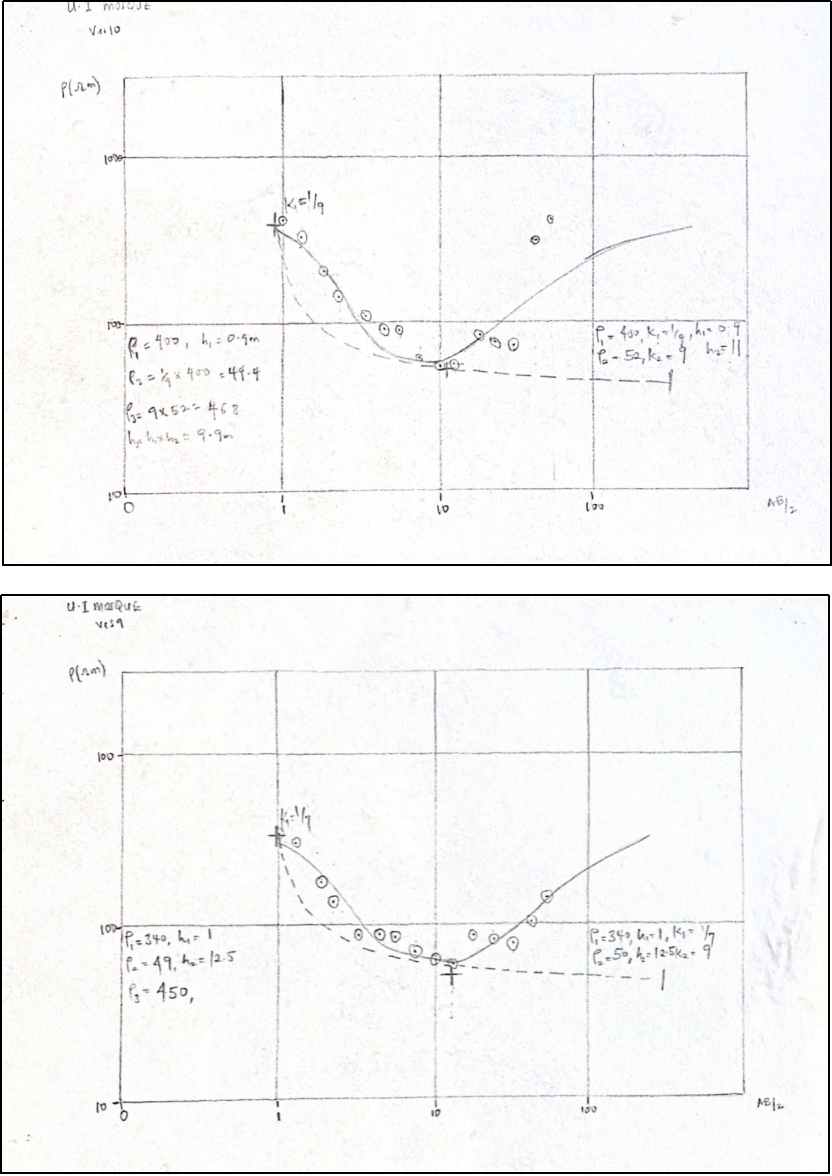
\includegraphics[width=0.85\textwidth]{Picture1.png}
    \caption{Some Curve Matching Rrepresentaion on log-log graph combined}
    \label{fig:Curve MAtching}
\end{figure}

\section{Vertical Electrical Sounding Data Interpretation}

\subsection{VES 1 Station at UI Mosque}

\begin{figure}[H]
    \centering
    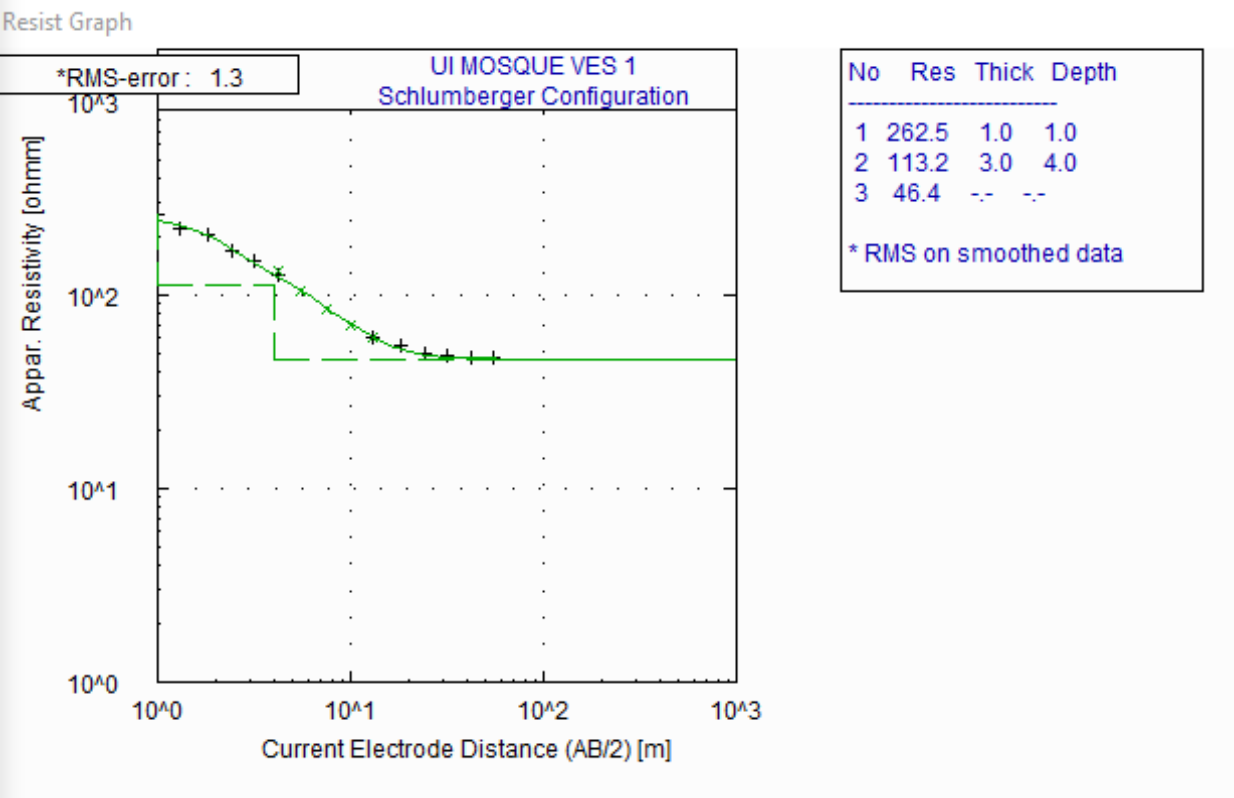
\includegraphics[width=1.0\textwidth]{ui_ves1.png}
    \caption{Graphical Rrepresentaion of VES 1}
    \label{fig:VES_1_Curve}
\end{figure}

The VES curve for UI Mosque VES 1 suggests an \textbf{Q-type pattern}, characterized by a descending resistivity trend, indicating a three-layer subsurface model. The first layer, with a resistivity of 262.5~$\Omega$m and a thickness of 1.0~m, represents the topsoil, likely composed of dry sandy soil or lateritic materials. Below this is the intermediate layer, which has a resistivity of 113.2~$\Omega$m and a thickness of 3.0~m, likely indicating clayey soil or moist sandy material due to its more conductive nature. The third layer, with a resistivity of 46.4~$\Omega$m and undefined thickness, is interpreted as a basement layer consisting of fractured or weathered rock, potentially saturated with water.

The subsurface lithology suggests a dry and resistive topsoil, a more conductive clay-rich intermediate layer, and a water-saturated or fractured basement rock. No significant faulting is apparent in the data, but the low resistivity of the third layer indicates high moisture content or fractures, which could affect foundation stability. While the top layer is stable, its thinness limits its load-bearing capacity. The intermediate layer’s compressible clay content may not support heavy foundations without proper treatment. The bottom layer’s water saturation or fractured condition warrants further geotechnical investigation to ensure suitability for construction.

\subsection{VES 2 Station at UI Mosque}

\begin{figure}[H]
    \centering
    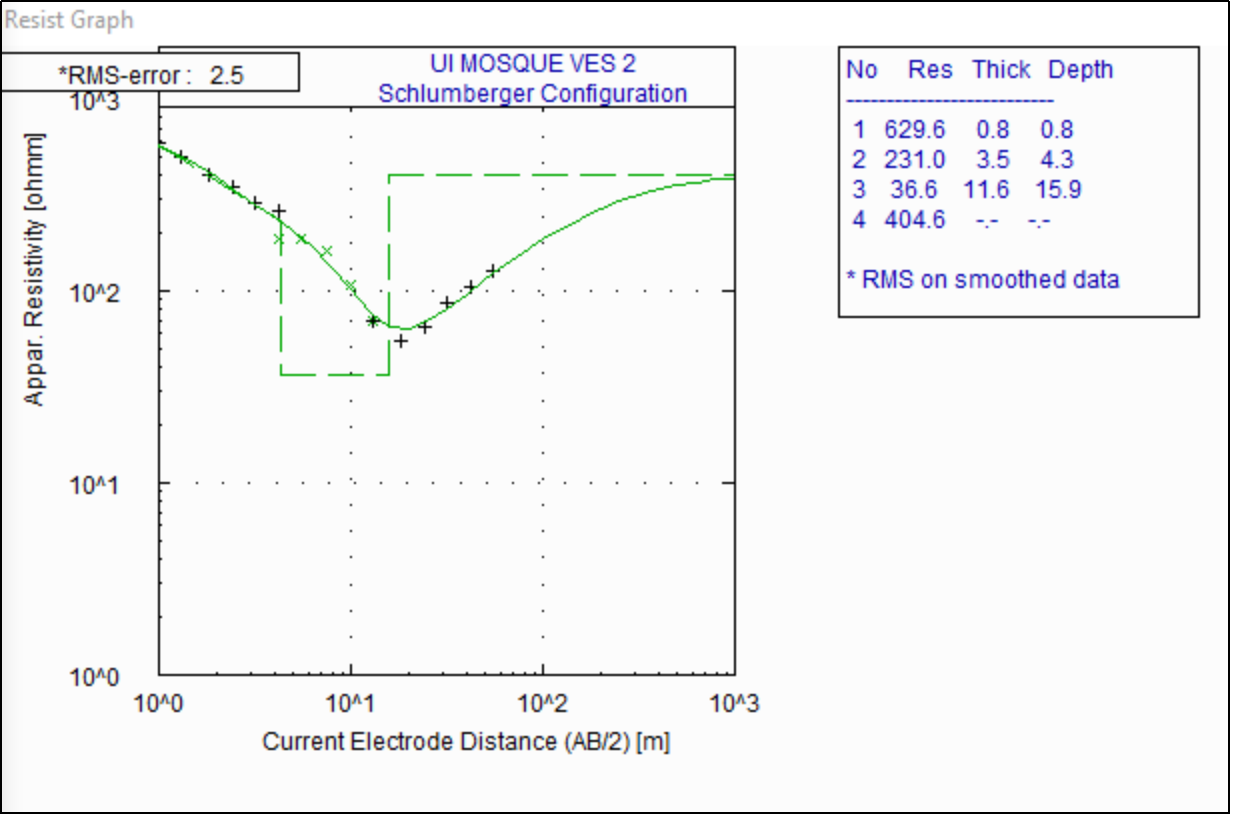
\includegraphics[width=1.0\textwidth]{ui_ves2.png}
    \caption{Graphical Rrepresentaion of VES 2}
    \label{fig:VES_2_Curve}
\end{figure}

The curve exhibits a \textbf{QH-type trend}, characterized by an initial descent in resistivity, followed by an ascent, and then another descent. This indicates a four-layer subsurface model with alternating resistive and conductive layers. The resistivity and thickness data for each layer are as follows: Layer 1 (Topsoil) has a resistivity of 629.6 $\Omega$ m and a thickness of 0.8 m, corresponding to a depth of 0.8 m. Layer 2 (Intermediate) has a resistivity of 231.0 $\Omega$ m and a thickness of 3.5 m, reaching a depth of 4.3 m. Layer 3 (Basement Transition) exhibits a resistivity of 36.6 $\Omega$ m and a thickness of 11.6 m, extending to a depth of 15.9 m. Finally, Layer 4 (Basement Rock) has a resistivity of 404.6 $\Omega$ m, but its thickness and depth are not specified. The subsurface lithology can be described as follows: Layer 1 (Topsoil) is dry and resistive, likely composed of sand or laterite; Layer 2 (Intermediate) is moderately resistive, suggesting weathered rock or moist sandy material; Layer 3 (Transition Zone) is highly conductive, likely consisting of clay-rich or water-saturated soil; and Layer 4 (Basement) is resistive, representing fractured or fresh bedrock rock.

For foundation suitability, Layer 1 (0--0.8 m) is suitable for shallow foundations if compacted. Layer 2 (0.8--4.3 m) may require evaluation for stability. Layer 3 (4.3--15.9 m) presents poor foundation conditions due to low resistivity, indicating potential compressibility or water saturation, necessitating deep foundations (e.g., piles). Layer 4 (below 15.9 m) is ideal for foundation support if bedrock is confirmed.
\subsection{VES 3 Station at UI Mosque}

\begin{figure}[H]
    \centering
    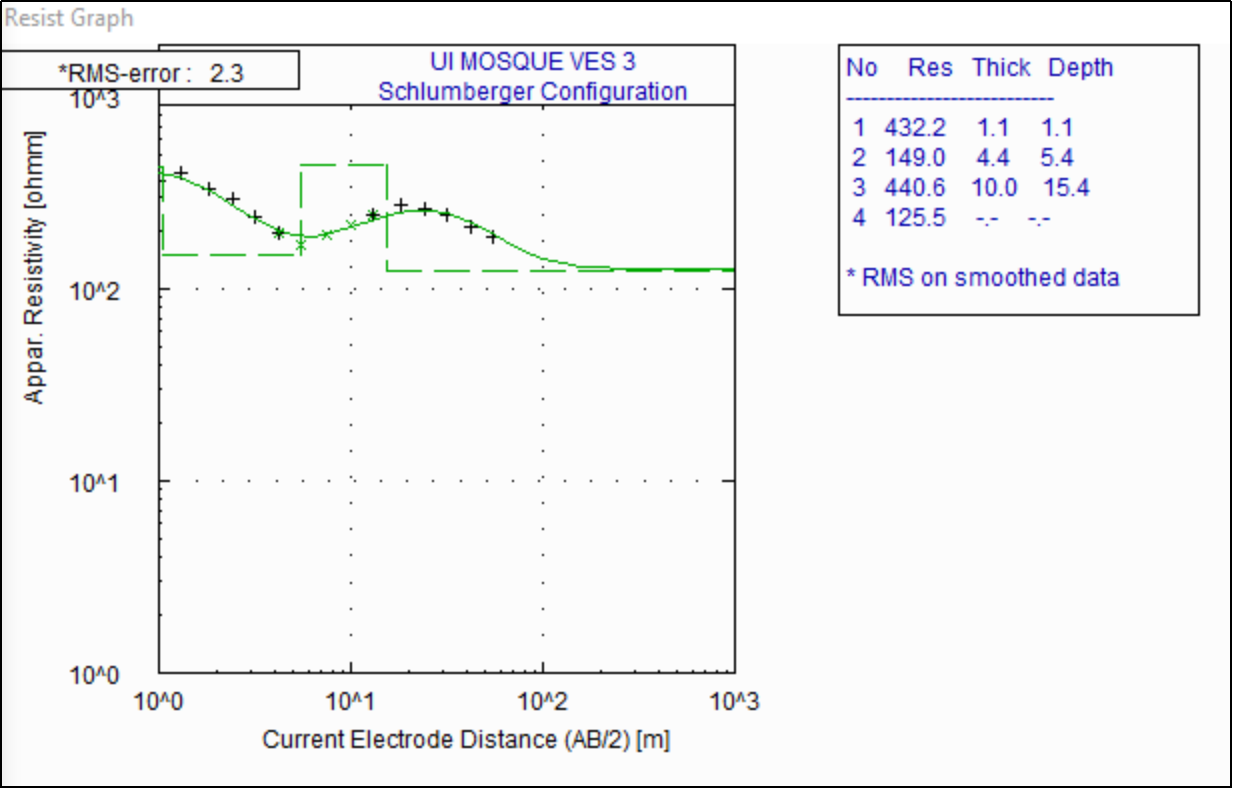
\includegraphics[width=1.0\textwidth]{ui_ves3.png}
    \caption{Graphical Rrepresentaion of VES 3}
    \label{fig:VES_3_Curve}
\end{figure}

The resistivity pattern indicates a \textbf{H-Type Curve}. The resistivity and thickness data for the layers are as follows: Layer 1 has a resistivity of 432.2 $\Omega\cdot$m and a thickness of 1.1 m, corresponding to a depth of 1.1 m. Layer 2 has a resistivity of 149.0 $\Omega\cdot$m and a thickness of 4.4 m, extending to a depth of 5.4 m. Layer 3 has a resistivity of 440.6 $\Omega\cdot$m and a thickness of 10.0 m, reaching a depth of 15.4 m. Layer 4 has a resistivity of 125.5 $\Omega\cdot$m and extends beyond the measured depth. The lithology interpretation suggests that Layer 1, with high resistivity, represents dry or compacted material, such as laterite or dry sand. Layer 2, with lower resistivity, could indicate clay or water-saturated soil. Layer 3, with increased resistivity, suggests compacted rock or unsaturated sandstone. Layer 4, with lower resistivity, points to a water-bearing formation or weathered rock.

For foundation suitability, Layer 1 (0--1.1 m) is suitable for shallow foundations if compact. Layer 2 (1.1--5.4 m) requires evaluation due to possible instability. Layer 3 (5.4--15.4 m) is more stable for deep foundations. Layer 4 below 15.4m should be assessed for load-bearing capacity before construction.

\subsection{VES 4 Station at UI Mosque}

\begin{figure}[H]
    \centering
    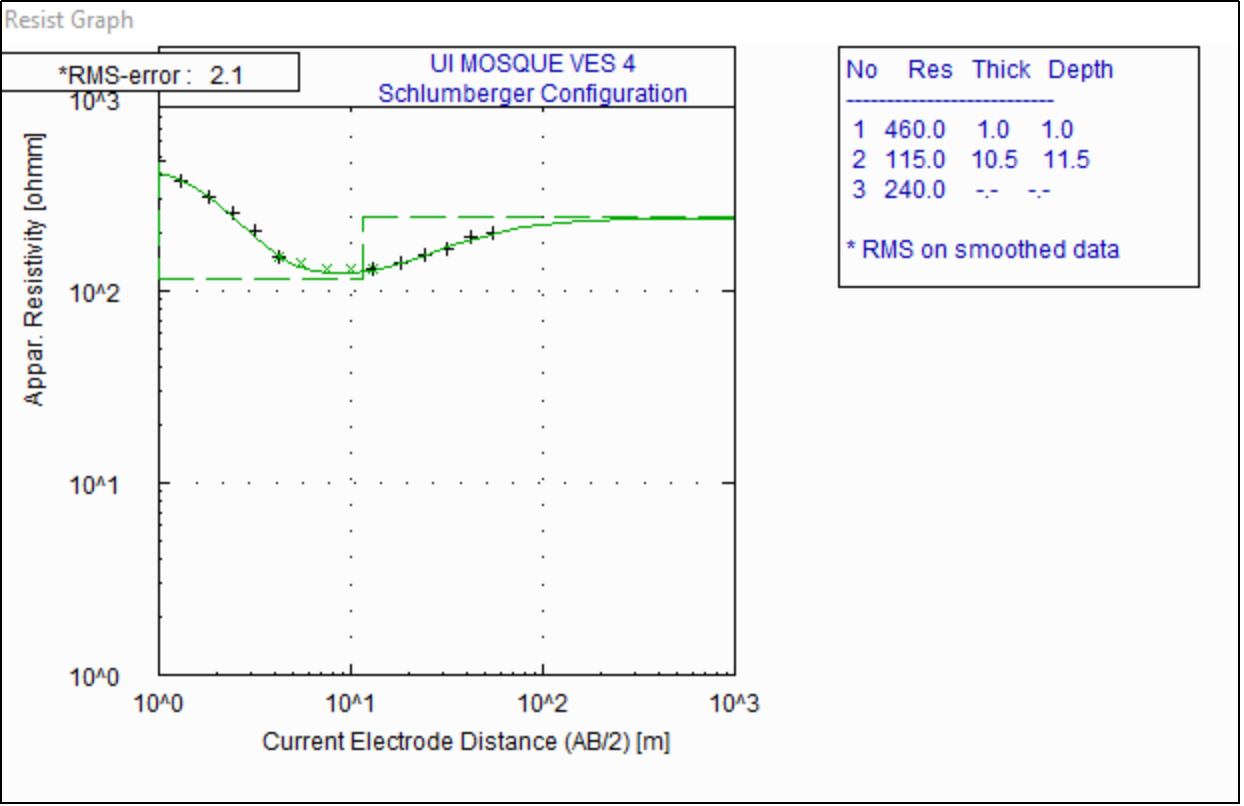
\includegraphics[width=1.0\textwidth]{ui_ves4.png}
    \caption{Graphical Rrepresentaion of VES 4}
    \label{fig:VES_4_Curve}
\end{figure}

The resistivity data indicates that the resistivity drops significantly from Layer 1 to Layer 2, and then partially increases in Layer 3. This suggests a \textbf{H-Type} curve with a transition zone between more resistive material and a moderately resistive layer. The resistivity and thickness data for the layers are as follows: Layer 1 has a resistivity of 460 $\Omega$ m and a thickness of 1.0 m, corresponding to a depth of 1.0 m. Layer 2 has a resistivity of 115.0 $\Omega$ m and a thickness of 10.5 m, extending to a depth of 11.5 m. Layer 3 has a resistivity of 240 $\Omega$ m, but its thickness and depth are not determined.

The lithology interpretation for the layers is as follows: Layer 1, with a high resistivity, could indicate dry, resistive material such as sand or laterite. Layer 2, with moderate resistivity, may suggest weathered rock or moist sandy material. Layer 3, with a higher resistivity than Layer 2 but lower than Layer 1, could represent fractured rock or a transition zone between weathered material and solid basement rock.

\subsection{VES 5 Station at UI Mosque}

\begin{figure}[H]
    \centering
    \includegraphics[width=1.0\textwidth]{ui_ves5.png}
    \caption{Graphical Rrepresentaion of VES 5}
    \label{fig:VES_5_Curve}
\end{figure}

This curve is typical \textbf{H-Type} curve, the resistivity and thickness data for the layers are as follows: Layer 1 has a resistivity of 220 $\Omega$ m and a thickness of 1.0 m, corresponding to a depth of 1.0 m. Layer 2 has a resistivity of 94.3 $\Omega$ m and a thickness of 21.0 m, extending to a depth of 22.0 m. Layer 3 has a resistivity of 364 $\Omega$ m, but its thickness and depth not determined

The lithology interpretation for the layers is as follows: Layer 1, with a relatively moderate resistivity, may represent a type of soil or weathered material such as sand or laterite. Layer 2, with a significantly lower resistivity, likely indicates a conductive layer such as clay, water-saturated soil, or a more saturated transition zone. Layer 3, with a higher resistivity, may correspond to solid rock, possibly fractured basement rock or dry, resistive material beneath the conductive zone.

\subsection{VES 6 Station at UI Mosque}

\begin{figure}[H]
    \centering
    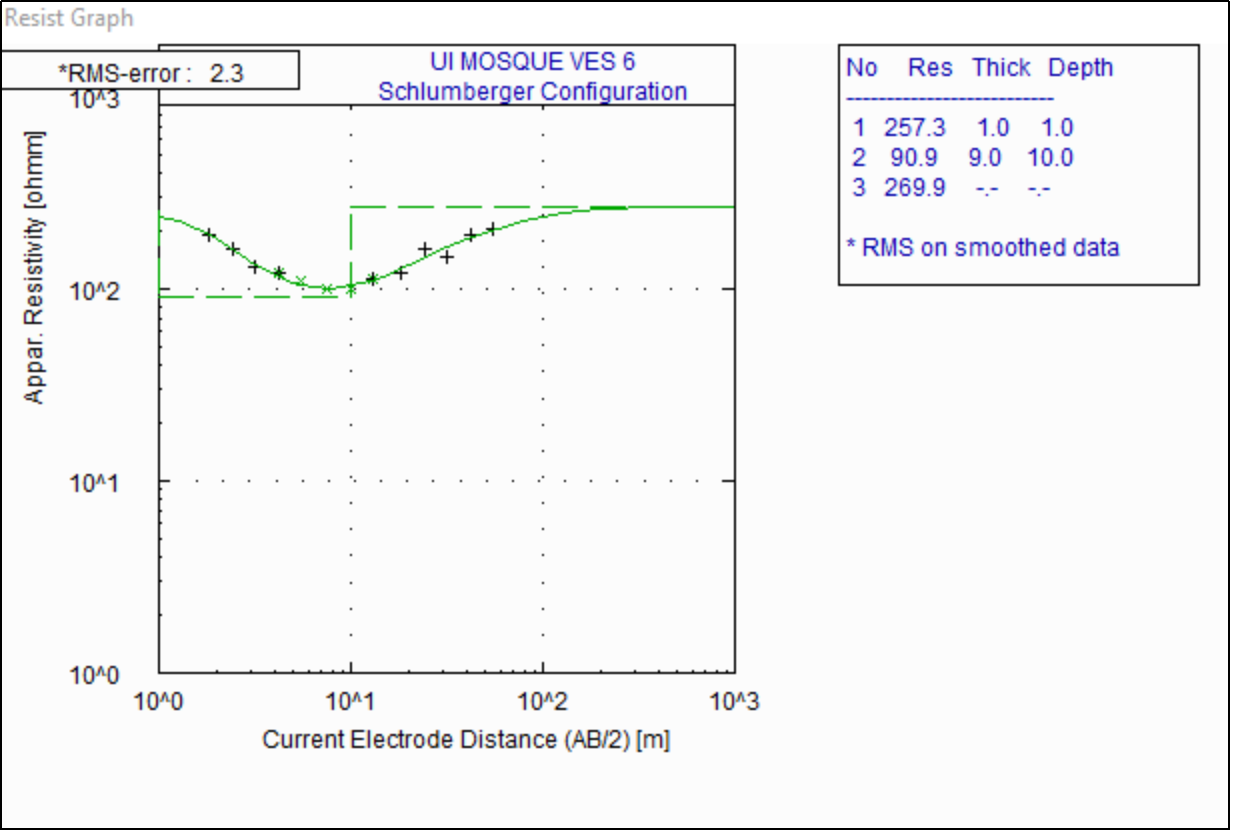
\includegraphics[width=1.0\textwidth]{ui_ves6.png}
    \caption{Graphical Rrepresentaion of VES 6}
    \label{fig:VES_6_Curve}
\end{figure}

The resistivity and thickness data for the layers are as follows: Layer 1 has a resistivity of 257.3 $\Omega$ m and a thickness of 1.0 m, corresponding to a depth of 1.0 m. Layer 2 has a resistivity of 90.9 $\Omega$ m and a thickness of 9.0 m, extending to a depth of 10.0 m. Layer 3 has a resistivity of 269.9 $\Omega$ m, but its thickness and depth are not determined.

The lithology interpretation for the layers is as follows: Layer 1, with a relatively high resistivity, could represent dry, resistive material such as sand or laterite. Layer 2, with a lower resistivity, likely represents a conductive layer, such as clay, moist sandy material, or water-saturated soil. Layer 3, with a resistivity similar to Layer 1, suggests a return to resistive conditions, possibly indicating a transition to a solid or fractured basement rock. This is typical \textbf{H-Type} curves.

\subsection{VES 7 Station at UI Mosque}

\begin{figure}[H]
    \centering
    \includegraphics[width=1.0\textwidth]{ui_ves7.png}
    \caption{Graphical Rrepresentaion of VES 7}
    \label{fig:VES_7_Curve}
\end{figure}

The resistivity decreases in Layer 2 and then increases again in Layer 3, suggesting a \textbf{H-Type} curve with a conductive layer (Layer 2) beneath a resistive top layer (Layer 1) and a return to resistivity at greater depth (Layer 3). The resistivity and thickness data for the layers are as follows: Layer 1 has a resistivity of 416.8 $\Omega$ m and a thickness of 1.1 m, corresponding to a depth of 1.1 m. Layer 2 has a resistivity of 80.5 $\Omega$ m and a thickness of 10.6 m, extending to a depth of 11.6 m. Layer 3 has a resistivity of 320.1 $\Omega$m.

The lithology interpretation for the layers is as follows: Layer 1, with a high resistivity, likely represents dry, resistive material such as sand or laterite. Layer 2, with a significantly lower resistivity, is likely to be a conductive zone, such as clay, water-saturated soil, or a weathered material. Layer 3, with a higher resistivity than Layer 2, could represent fractured rock or solid basement rock, which is more resistive than the overlying conductive material.

\subsection{VES 8 Station at UI Mosque}

\begin{figure}[H]
    \centering
    \includegraphics[width=1.0\textwidth]{ui_ves8.png}
    \caption{Graphical Rrepresentaion of VES 8}
    \label{fig:VES_8_Curve}
\end{figure}

The resistivity decreases significantly from Layer 1 to Layer 2 and further decreases in Layer 3, which suggests a three-layer curve with a progressively more conductive layer at greater depths. This pattern is indicative of a \textbf{Q-Type} curve. The resistivity and thickness data for the layers are as follows: Layer 1 has a resistivity of 349.7 $\Omega$ m and a thickness of 1.0 m, corresponding to a depth of 1.0 m. Layer 2 has a resistivity of 122.2 $\Omega$ m and a thickness of 6.6 m, extending to a depth of 7.6 m. Layer 3 has a resistivity of 27.7 $\Omega$m.

The lithology interpretation for the layers is as follows: Layer 1, with a relatively high resistivity, likely represents dry, resistive material such as sand or laterite. Layer 2, with moderate resistivity, could represent weathered rock, moist sandy material, or a transition zone. Layer 3, with a very low resistivity, suggests a conductive layer, possibly clay-rich, water-saturated soil, or a highly conductive transition zone.

\subsection{VES 9 Station at UI Mosque}

\begin{figure}[H]
    \centering
    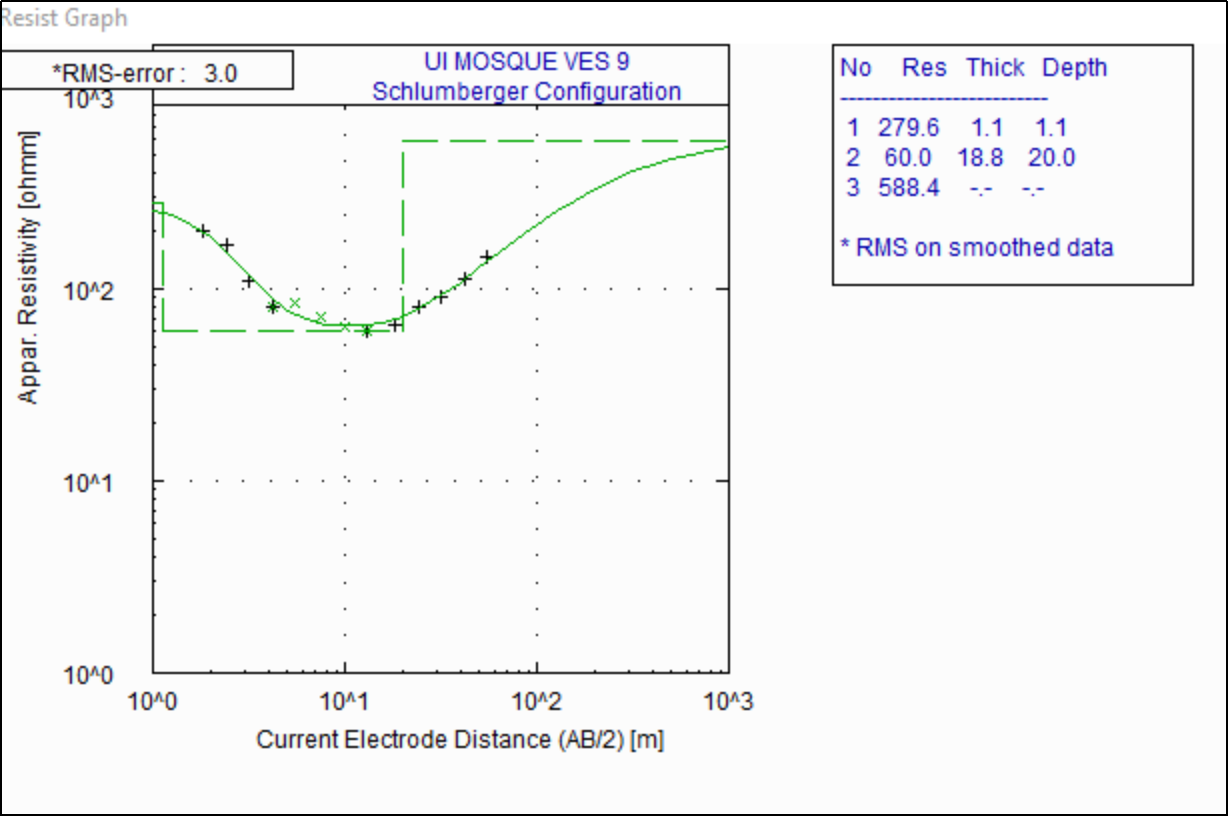
\includegraphics[width=1.0\textwidth]{ui_ves9.png}
    \caption{Graphical Rrepresentaion of VES 9}
    \label{fig:VES_9_Curve}
\end{figure}

The resistivity pattern indicates a \textbf{K-Type Curve}. The resistivity and thickness data for the layers are as follows: Layer 1 has a resistivity of 279.6 $\Omega\cdot$m and a thickness of 1.1 m, corresponding to a depth of 1.1 m. Layer 2 has a resistivity of 60.0 $\Omega\cdot$m and a thickness of 18.8 m, extending to a depth of 19.9 m. Layer 3 has a resistivity of 588.4 $\Omega\cdot$m and extends beyond the measured depth. This pattern is typical of geological settings where a resistive layer (e.g., dry sand/gravel) overlies a conductive layer (e.g., clay or water-saturated soil) and is underlain by a highly resistive layer (e.g., bedrock).

For foundation suitability, Layer 1 (0--1.1 m) is suitable for shallow foundations if compacted, but may require removal if loose or unstable. Layer 2 (1.1--19.9 m) presents poor foundation conditions due to low resistivity, indicating potential compressibility or water saturation, necessitating deep foundations (e.g., piles) to bypass this layer. Layer 3 (below 19.9 m) is ideal for foundation support if bedrock is confirmed, as it provides a stable and strong base.
\subsection{VES 10 Station at UI Mosque}

\begin{figure}[H]
    \centering
    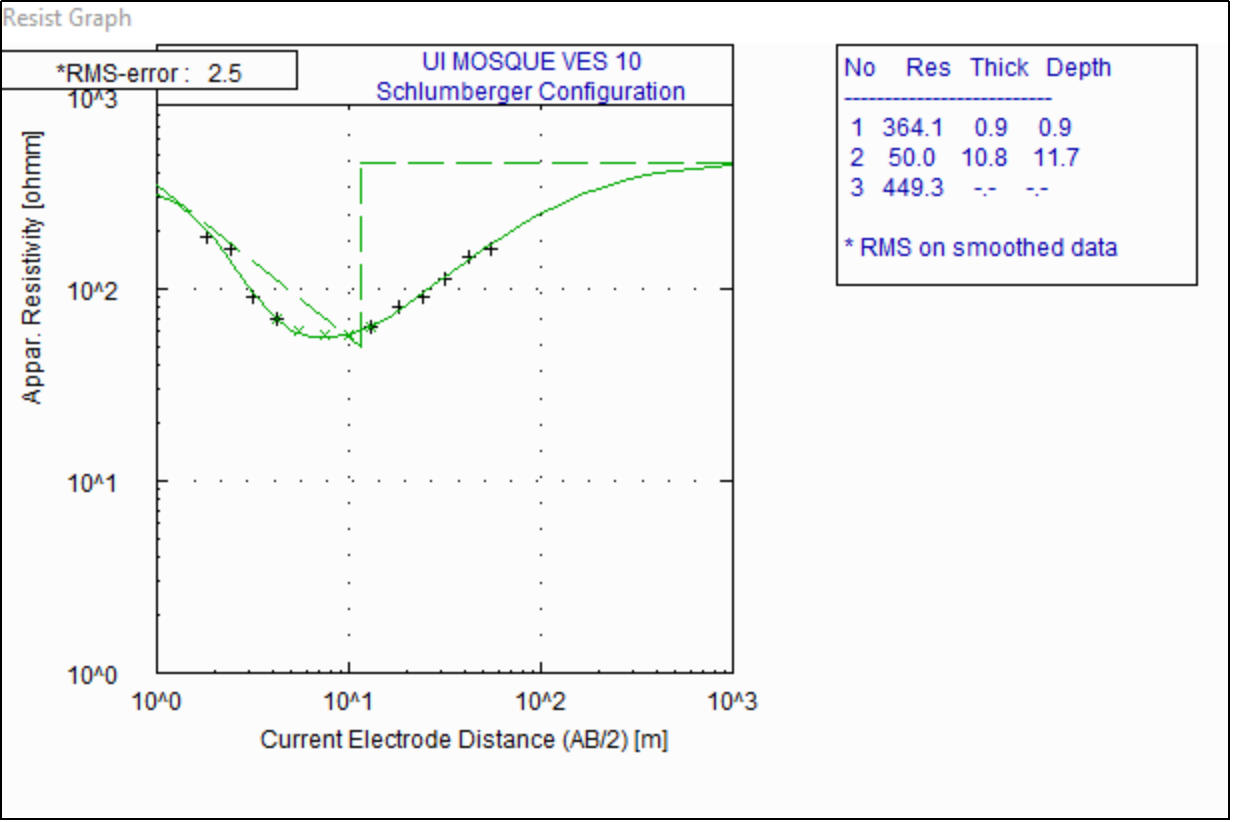
\includegraphics[width=1.0\textwidth]{ui_ves10.png}
    \caption{Graphical Rrepresentaion of VES 10}
    \label{fig:VES_10_Curve}
\end{figure}

The resistivity pattern indicates an \textbf{H-Type Curve}, characterized by a low-resistivity layer (Layer 2) sandwiched between two high-resistivity layers (Layer 1 and Layer 3). This is typical of geological settings where a conductive layer (e.g., clay or water-saturated soil) is overlain and underlain by more resistive materials (e.g., dry sand/gravel and bedrock). The resistivity and thickness data for the layers are as follows: Layer 1 has a resistivity of 364.1 $\Omega\cdot$m and a thickness of 0.9 m, corresponding to a depth of 0.9 m. Layer 2 has a resistivity of 50.0 $\Omega\cdot$m and a thickness of 10.8 m, extending to a depth of 11.7 m. Layer 3 has a resistivity of 449.3 $\Omega\cdot$m and extends beyond the measured depth. The lithology interpretation suggests that Layer 1, with high resistivity, likely represents dry or resistive material, such as gravel or dry sand. Layer 2, with significantly lower resistivity, indicates a conductive layer, which could be clay-rich soil or water-saturated sand. Layer 3, with very high resistivity, suggests bedrock or dense, compacted material.

For foundation suitability, Layer 1 (0--0.9 m) is suitable for shallow foundations if compacted, but may require removal if loose or unstable. Layer 2 (0.9--11.7 m) presents poor foundation conditions due to low resistivity, indicating potential compressibility or water saturation, necessitating deep foundations (e.g., piles) to bypass this layer. Layer 3 (below 11.7 m) is ideal for foundation support if bedrock is confirmed, as it provides a stable and strong base.

\subsection{VES 1 Station at AAH}

\begin{figure}[H]
    \centering
    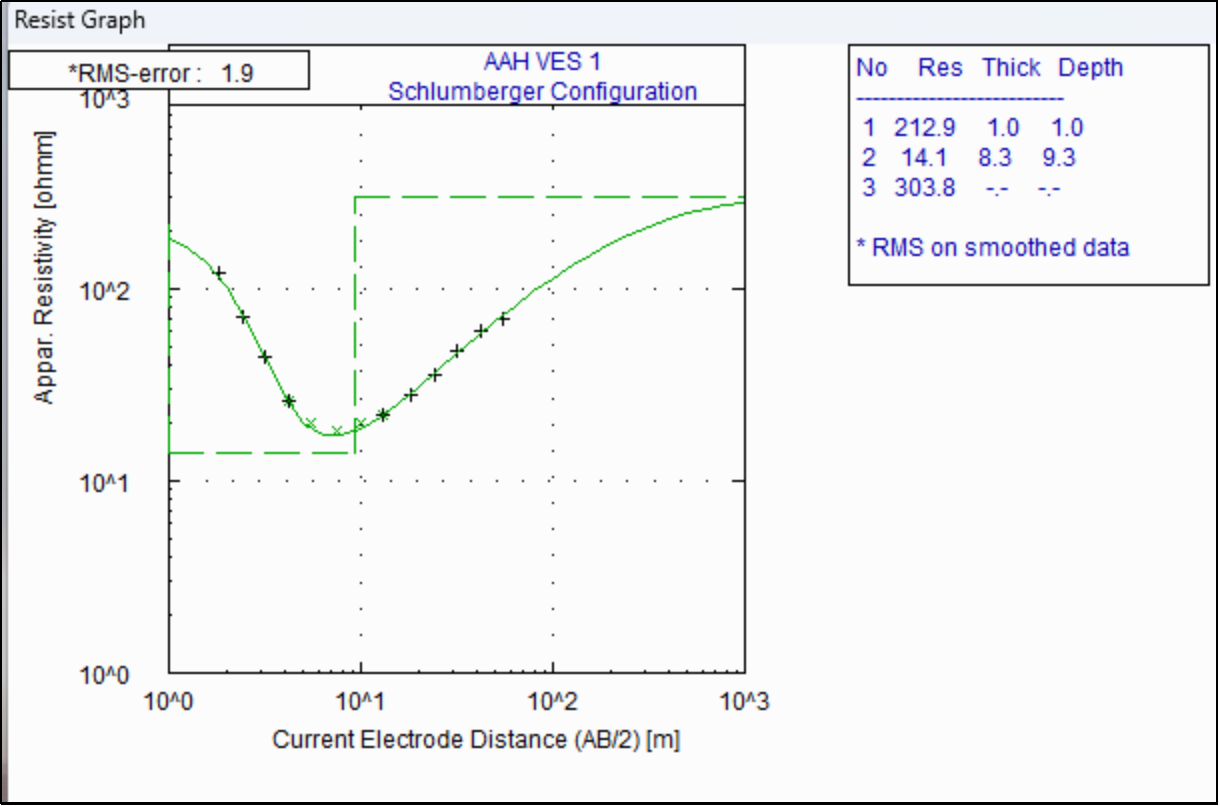
\includegraphics[width=1.0\textwidth]{aah_ves1.png}
    \caption{Graphical Rrepresentaion of VES 1}
    \label{fig:AAH_VES_1_Curve}
\end{figure}

The resistivity significantly drops in Layer 2 and then increases in Layer 3, which aligns with the \textbf{H-Type Curve}. This is characterized by a low-resistivity layer (Layer 2) sandwiched between two high-resistivity layers (Layer 1 and Layer 3). This configuration is typical for weathered basement or clay layers underlain by fresh bedrock. The resistivity and thickness data for the layers are as follows: Layer 1 has a resistivity of 212.9 $\Omega$ m and a thickness of 1.0 m, corresponding to a depth of 1.0 m. Layer 2 has a resistivity of 14.1 $\Omega$ m and a thickness of 8.3 m, extending to a depth of 9.3 m. Layer 3 has a resistivity of 303.8 $\Omega$m.

The lithology interpretation for the layers is as follows: Layer 1, with moderate resistivity, likely represents dry, resistive material such as sand or laterite. Layer 2, with a very low resistivity, suggests a conductive layer, possibly clay-rich, water-saturated soil, or a highly weathered zone. Layer 3, with high resistivity, indicates a return to resistive material, likely fractured rock or fresh basement.

\subsection{VES 2 Station at AAH}

\begin{figure}[H]
    \centering
    \includegraphics[width=1.0\textwidth]{aah_ves2.png}
    \caption{Graphical Rrepresentaion of VES 2}
    \label{fig:AAH_VES_2_Curve}
\end{figure}

The resistivity and thickness data for the layers are as follows: Layer 1 has a resistivity of 476.3 $\Omega$ m and a thickness of 0.8 m. Layer 2 has a resistivity of 13.6 $\Omega$ m and a thickness of 3.0 m. Layer 3 has a resistivity of 556.0 $\Omega$ m. The resistivity decreases significantly in Layer 2 and then increases again in Layer 3, suggesting an \textbf{H-Type Curve}. This is typical of a low-resistivity layer (Layer 2) sandwiched between two high-resistivity layers (Layer 1 and Layer 3), often indicative of a weathered basement or clay layer beneath resistive material.

The lithology interpretation for the layers is as follows: Layer 1, with high resistivity, likely represents dry, resistive material such as sand or laterite. Layer 2, with very low resistivity, indicates a conductive layer, likely clay-rich, water-saturated soil, or weathered material. Layer 3, with a very high resistivity, suggests solid or fractured basement rock.

\subsection{VES 3 Station at AAH}

\begin{figure}[H]
    \centering
    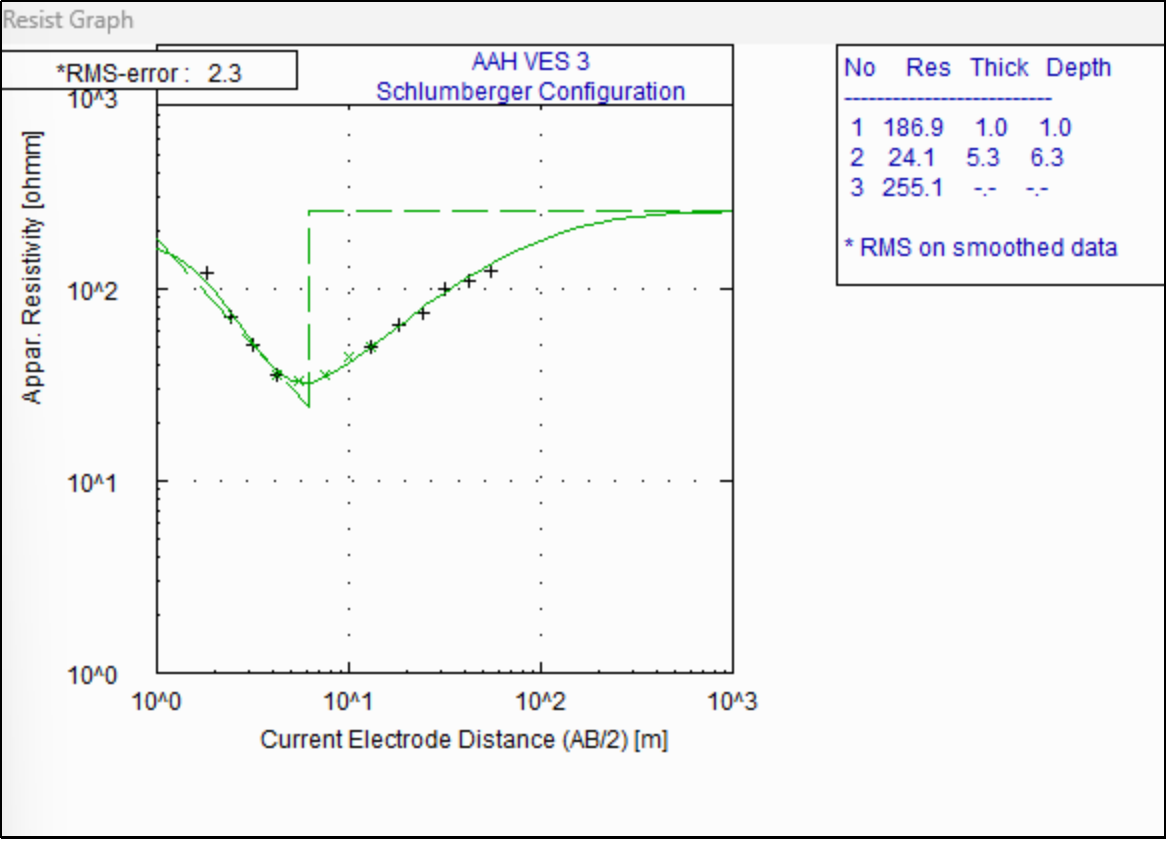
\includegraphics[width=1.0\textwidth]{aah_ves3.png}
    \caption{Graphical Rrepresentaion of VES 3}
    \label{fig:AAH_VES_3_Curve}
\end{figure}
The resistivity and thickness data for the layers are as follows: Layer 1 has a resistivity of 186.9 $\Omega$ m and a thickness of 1.0 m, corresponding to a depth of 1.0 m. Layer 2 has a resistivity of 24.1 $\Omega$ m and a thickness of 5.3 m, extending to a depth of 6.3 m. Layer 3 has a resistivity of 255.1 $\Omega$ m. The lithology interpretation suggests that Layer 1, with moderate resistivity, likely represents dry, resistive material such as sand or laterite. Layer 2, with very low resistivity, indicates a conductive layer, possibly clay-rich, water-saturated soil, or a weathered zone. Layer 3, with high resistivity, points to solid or fractured basement rock. The resistivity decreases in Layer 2 and then increases again in Layer 3, aligning with an \textbf{H-Type Curve}, which is characterized by a low-resistivity layer (Layer 2) sandwiched between two high-resistivity layers (Layer 1 and Layer 3), typically indicative of weathered basement or clay layers underlain by fresh bedrock.

\subsection{VES 4 Station at AAH}

\begin{figure}[H]
    \centering
    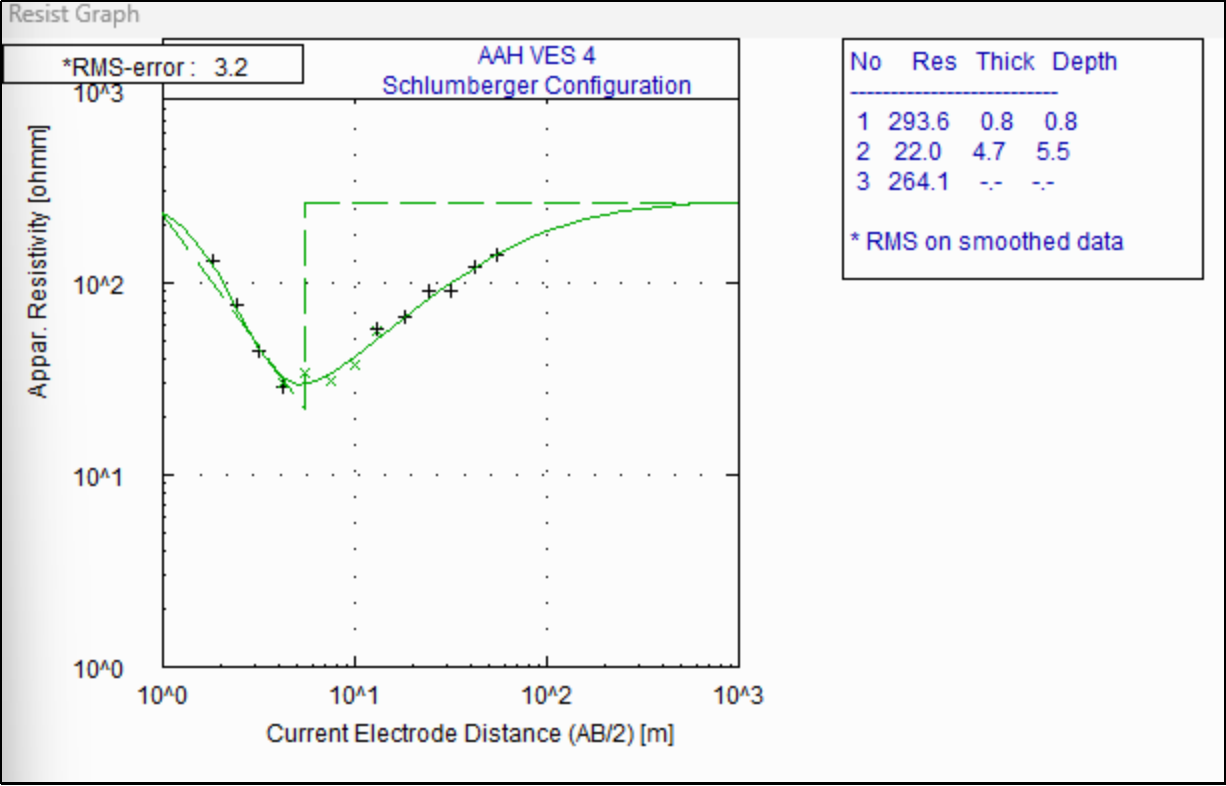
\includegraphics[width=1.0\textwidth]{aah_ves4.png}
    \caption{Graphical Rrepresentaion of VES 4}
    \label{fig:AAH_VES_4_Curve}
\end{figure}
The resistivity and thickness data for the layers are as follows: Layer 1 has a resistivity of 293.6 $\Omega$ m and a thickness of 0.8 m, corresponding to a depth of 0.8 m. Layer 2 has a resistivity of 22.0 $\Omega$ m and a thickness of 4.7 m, extending to a depth of 5.5 m. Layer 3 has a resistivity of 264.1 $\Omega$ m.

The lithology interpretation suggests that Layer 1, with high resistivity, likely represents dry, resistive material such as sand or laterite. Layer 2, with a much lower resistivity, indicates a conductive layer, possibly clay-rich, water-saturated soil, or a weathered zone. Layer 3, with moderate resistivity, likely represents a transition to solid or fractured basement rock. The resistivity decreases in Layer 2 and then increases in Layer 3, aligning with an \textbf{H-Type Curve}, characterized by a low-resistivity layer (Layer 2) sandwiched between two high-resistivity layers (Layer 1 and Layer 3), which is typically indicative of a weathered basement or clay layer beneath resistive material.

\subsection{VES 5 Station at AAH}

\begin{figure}[H]
    \centering
    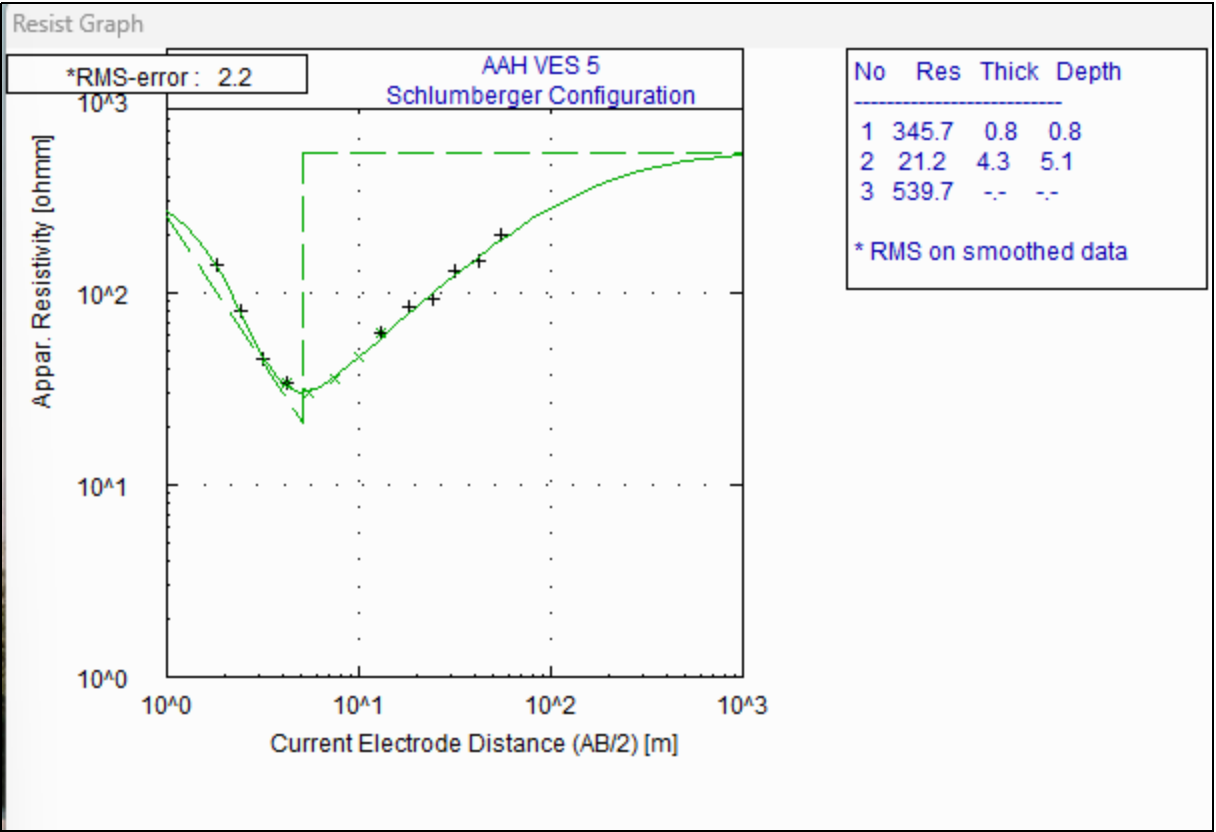
\includegraphics[width=1.0\textwidth]{aah_ves5.png}
    \caption{Graphical Rrepresentaion of VES 5}
    \label{fig:AAH_VES_5_Curve}
\end{figure}
The resistivity and thickness data for the layers are as follows: Layer 1 has a resistivity of 345.7 $\Omega$ m and a thickness of 0.8 m, corresponding to a depth of 0.8 m. Layer 2 has a resistivity of 21.2 $\Omega$ m and a thickness of 4.3 m, extending to a depth of 5.1 m. Layer 3 has a resistivity of 539.7 $\Omega$ m. The lithology interpretation suggests that Layer 1, with high resistivity, likely represents dry, resistive material such as sand or laterite. Layer 2, with much lower resistivity, indicates a conductive layer, possibly clay-rich, water-saturated soil, or a weathered zone. Layer 3, with a very high resistivity, suggests solid or fractured basement rock.

The resistivity decreases in Layer 2 and then increases in Layer 3, indicating an \textbf{H-Type Curve}, characterized by a low-resistivity layer (Layer 2) sandwiched between two high-resistivity layers (Layer 1 and Layer 3), typical of weathered basement or clay layers underlain by fresh bedrock.

\subsection{VES 6 Station at AAH}

\begin{figure}[H]
    \centering
    \includegraphics[width=1.0\textwidth]{aah_ves6.png}
    \caption{Graphical Rrepresentaion of VES 6}
    \label{fig:AAH_VES_6_Curve}
\end{figure}
The resistivity and thickness data for the layers are as follows: Layer 1 has a resistivity of 368.7 $\Omega$ m and a thickness of 0.8 m, corresponding to a depth of 0.8 m. Layer 2 has a resistivity of 30.7 $\Omega$ m and a thickness of 8.2 m, extending to a depth of 8.9 m. Layer 3 has a resistivity of 596.1 $\Omega$ m. The lithology interpretation suggests that Layer 1, with high resistivity, likely represents dry, resistive material such as sand or laterite. Layer 2, with a lower resistivity, indicates a conductive layer, possibly clay-rich, water-saturated soil, or a weathered zone. Layer 3, with very high resistivity, suggests solid or fractured basement rock. 

The resistivity decreases in Layer 2 and then increases in Layer 3, aligning with an \textbf{H-Type Curve}, characterized by a low-resistivity layer (Layer 2) sandwiched between two high-resistivity layers (Layer 1 and Layer 3), indicative of a weathered basement or clay layer beneath resistive material.

\subsection{VES 7 Station at AAH}

\begin{figure}[H]
    \centering
    \includegraphics[width=1.0\textwidth]{aah_ves7.png}
    \caption{Graphical Rrepresentaion of VES 7}
    \label{fig:AAH_VES_7_Curve}
\end{figure}
The resistivity and thickness data for the layers are as follows: Layer 1 has a resistivity of 315.5 $\Omega$ m and a thickness of 1.0 m, corresponding to a depth of 1.0 m. Layer 2 has a resistivity of 40.1 $\Omega$ m and a thickness of 9.9 m, extending to a depth of 10.9 m. Layer 3 has a resistivity of 834.5 $\Omega$ m. The lithology interpretation suggests that Layer 1, with high resistivity, likely represents dry, resistive material such as sand or laterite. Layer 2, with much lower resistivity, indicates a conductive layer, possibly clay-rich, water-saturated soil, or a weathered zone. Layer 3, with very high resistivity, points to solid or fractured basement rock.

The resistivity decreases in Layer 2 and then increases again in Layer 3, fitting an \textbf{H-Type Curve}, characterized by a low-resistivity layer (Layer 2) sandwiched between two high-resistivity layers (Layer 1 and Layer 3), typically indicative of weathered basement or clay layers underlain by fresh bedrock.

\subsection{VES 8 Station at AAH}

\begin{figure}[H]
    \centering
    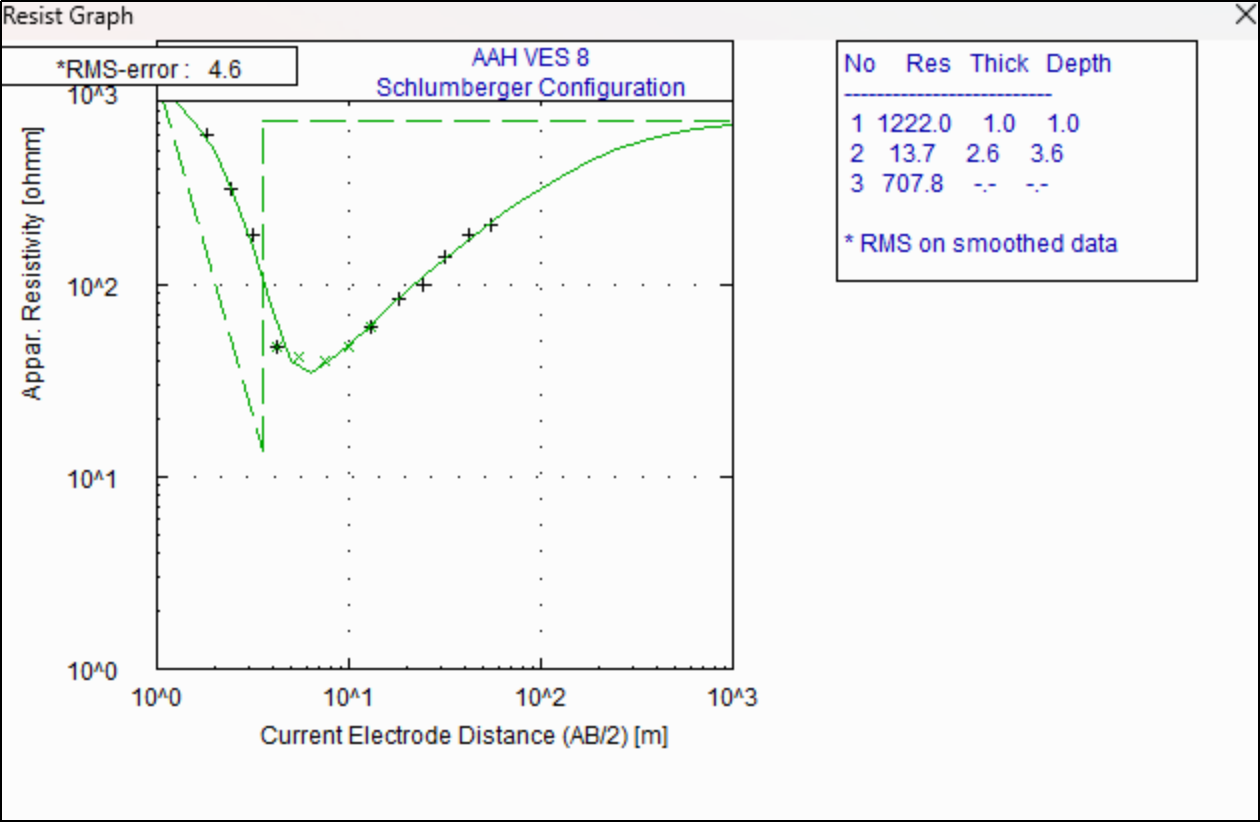
\includegraphics[width=1.0\textwidth]{aah_ves8.png}
    \caption{Graphical Rrepresentaion of VES 8}
    \label{fig:AAH_VES_8_Curve}
\end{figure}
The resistivity and thickness data for the layers are as follows: Layer 1 has a resistivity of 1222.0 $\Omega$ m and a thickness of 1.0 m, corresponding to a depth of 1.0 m. Layer 2 has a resistivity of 13.7 $\Omega$ m and a thickness of 2.6 m, extending to a depth of 3.6 m. Layer 3 has a resistivity of 707.8 $\Omega$ m. The lithology interpretation suggests that Layer 1, with very high resistivity, represents fresh bedrock or basement rock. Layer 2, with very low resistivity, indicates a conductive layer, likely clay-rich or water-saturated soil. Layer 3, with high resistivity, points to solid or fractured basement rock. The resistivity decreases in Layer 2 and then increases again in Layer 3, fitting an \textbf{H-Type Curve}, characterized by a low-resistivity layer (Layer 2) sandwiched between two high-resistivity layers (Layer 1 and Layer 3), indicative of a weathered basement or clay layer beneath resistive material.

\subsection{VES 9 Station at AAH}

\begin{figure}[H]
    \centering
    \includegraphics[width=1.0\textwidth]{aah_ves9.png}
    \caption{Graphical Rrepresentaion of VES 9}
    \label{fig:AAH_VES_9_Curve}
\end{figure}
The resistivity pattern indicates a \textbf{KHK-Type Curve}. The resistivity and thickness data for the layers are as follows: Layer 1 has a resistivity of 445.4 $\Omega\cdot$m and a thickness of 0.5m, corresponding to a depth of 0.5m.  
Layer 2 has a resistivity of 43.4 $\Omega\cdot$m and a thickness of 1.4 m, extending to a depth of 1.9 m.  
Layer 3 has a resistivity of 166.7 $\Omega\cdot$m and a thickness of 11.4 m, reaching a depth of 13.2 m.  
Layer 4 has a resistivity of 18.6 $\Omega\cdot$m and a thickness of 3.8 m, extending to a depth of 17.0 m.  
Layer 5 has a resistivity of 433.9 $\Omega\cdot$m and extends beyond the measured depth.  

The lithology interpretation suggests that: Layer 1, with high resistivity, represents dry or compacted material, such as laterite or dry sand.  
Layer 2, with significantly lower resistivity, could indicate clay or water-saturated soil.  
Layer 3, with increased resistivity, suggests compacted rock or unsaturated sandstone.  
Layer 4, with very low resistivity, points to a highly conductive, water-bearing formation or clayey material.  
Layer 5, with high resistivity, may represent a consolidated bedrock or a dry formation beneath the surveyed depth.  

For foundation suitability: Layer 1 (0--0.5 m) may be suitable for shallow foundations if compact.  
Layer 2 (0.5--1.9 m) requires evaluation due to possible instability.  
Layer 3 (1.9--13.2 m) is more stable and can support deep foundations.  
Layer 4 (13.2--17.0 m) should be assessed for load-bearing capacity before construction.  
Layer 5 (below 17.0 m) might be suitable for deep foundation anchorage, depending on its geological characteristics.  

\subsection{VES 10 Station at AAH}

\begin{figure}[H]
    \centering
    \includegraphics[width=1.0\textwidth]{aah_ves10.png}
    \caption{Graphical Rrepresentaion of VES 10}
    \label{fig:AAH_VES_10_Curve}
\end{figure}
The resistivity and thickness data for the layers are as follows: Layer 1 has a resistivity of 210.0 $\Omega$ m and a thickness of 0.7 m, corresponding to a depth of 0.7 m. Layer 2 has a resistivity of 70.0 $\Omega$ m and a thickness of 4.8 m, extending to a depth of 5.5 m. Layer 3 has a resistivity of 210.0 $\Omega$ m. The lithology interpretation suggests that Layer 1, with moderate resistivity, likely represents dry or resistive material. Layer 2, with lower resistivity, indicates a conductive layer, possibly clay-rich or water-saturated soil. Layer 3, with high resistivity, suggests solid or fractured basement rock. The resistivity pattern indicates an \textbf{H-Type Curve}, with a low-resistivity layer (Layer 2) sandwiched between two high-resistivity layers (Layer 1 and Layer 3), typical of weathered basement or clay-rich layers beneath resistive material.

\section{Constant Separation Traversing Data Interpretation}

\begin{figure}[H]
    \centering
    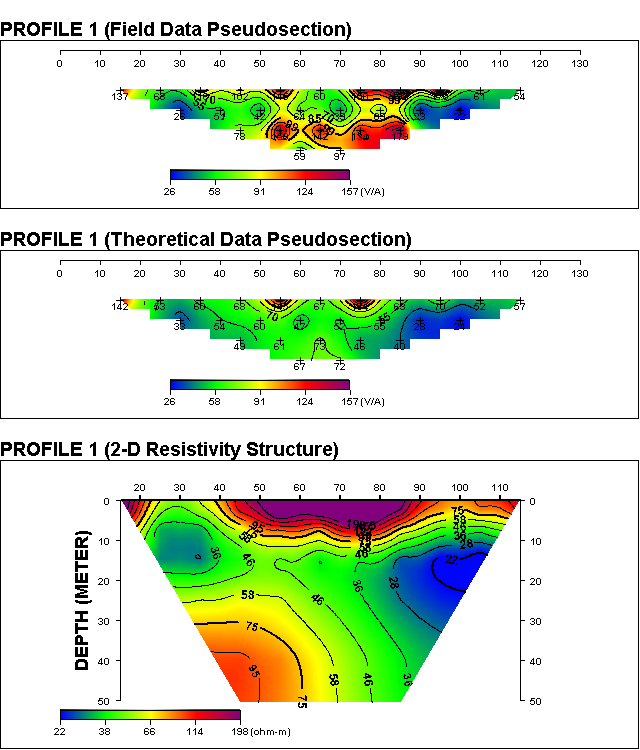
\includegraphics[width=1.0\textwidth]{PROFILE 1D.png}
    \caption{2D View of CST Profile 1}
    \label{fig:UI_CST_1_Curve}
\end{figure}

\begin{figure}[H]
    \centering
    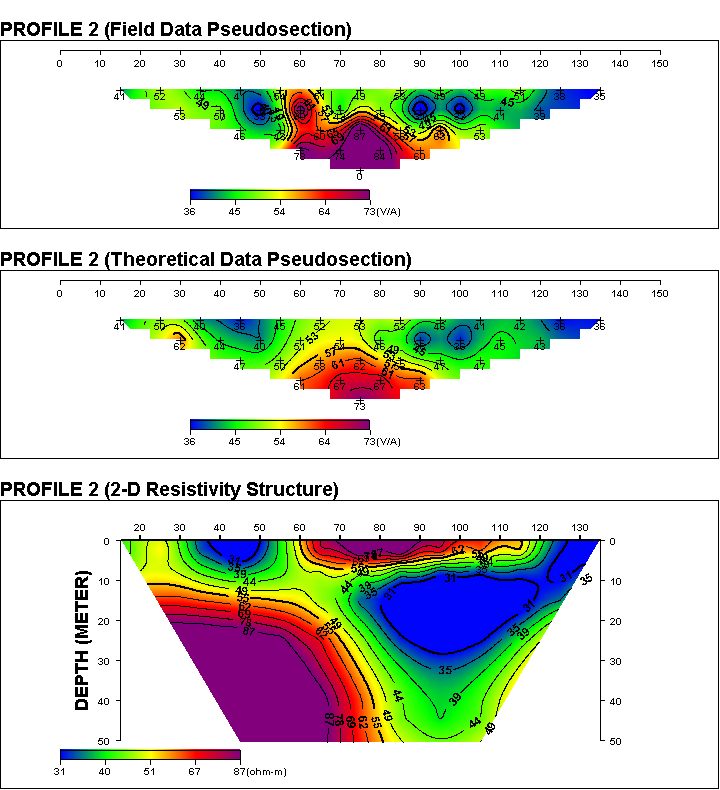
\includegraphics[width=1.0\textwidth]{PROFILE 2D.png}
    \caption{2D View of CST Profile 2}
    \label{fig:UI_CST_2_Curve}
\end{figure}

\begin{figure}[H]
    \centering
    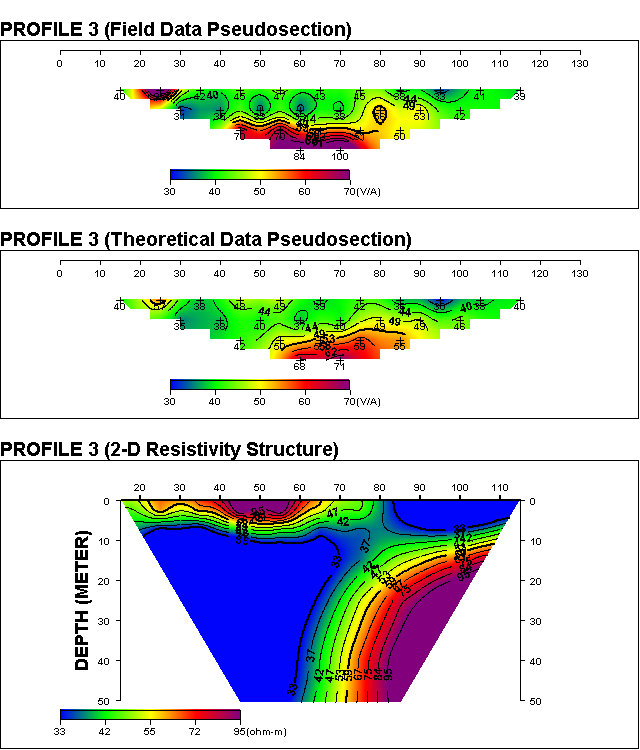
\includegraphics[width=1.0\textwidth]{PROFILE 3D.png}
    \caption{2D View of CST Profile 3}
    \label{fig:UI_CST_3_Curve}
\end{figure}

\begin{figure}[H]
    \centering
    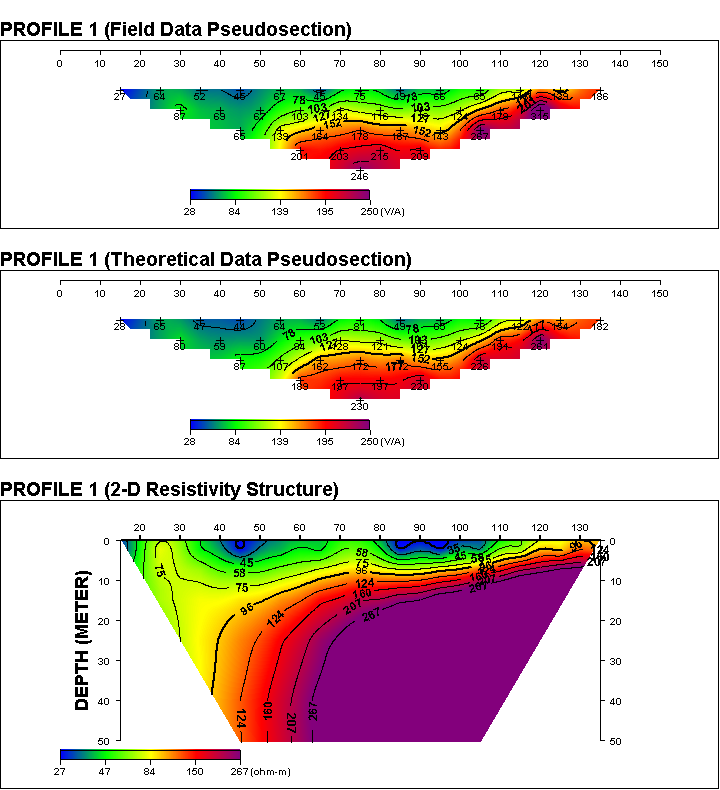
\includegraphics[width=1.0\textwidth]{PROFILE 1D (1).png}
    \caption{2D View of CST Profile 1 at AAH}
    \label{fig:AAH_CST_1_Curve}
\end{figure}

\begin{figure}[H]
    \centering
    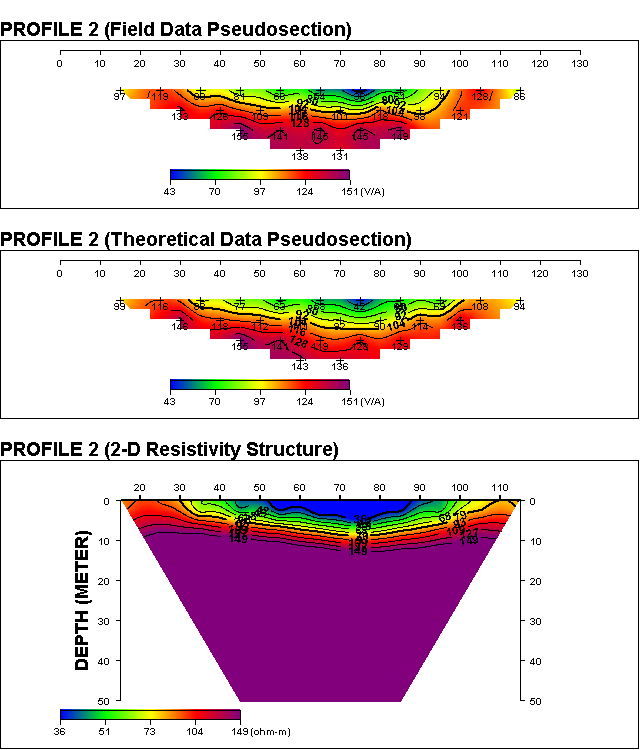
\includegraphics[width=1.0\textwidth]{PROFILE 2D (1).png}
    \caption{2D View of CST Profile 2 at AAH}
    \label{fig:aah_CST_2_Curve}
\end{figure}

\section{Interpretation of the Profiles}

\subsection{Resisitivity Variations}

\begin{enumerate}
    \item \textbf{Field Data Pseudosection:} Red colors (e.g., 250 V/A) indicate high resistivity, suggesting coarse-grained materials like sand and gravel. Blue colors (e.g., 26 V/A) suggest low resistivity, indicating saturated, fine-grained materials like clay or silt.

    \item \textbf{Theoretical Data Pseudosection:} Similar resistivity trends as the field data, with smoother variations.

    \item \textbf{2-D Resistivity Structure:} Red colors (e.g., 267 $\Omega$m) shown in Figure 4.27 represent high resistivity, while blue colors (e.g., 22 $\Omega$m) shown in Figure 4.24 represent low resistivity.

\end{enumerate}

\subsection{Profile 1 at UI Mosque}
Geological features inferred from the resistivity data include an estimated depth to bedrock around 50 meters, evidenced by increasing resistivity with depth. Abrupt changes in resistivity, such as transitions from low to high resistivity zones, may indicate potential faults or fractures. Low resistivity zones near the surface suggest areas with potential groundwater presence. For foundation design, high resistivity zones likely indicate coarse-grained soils suitable for bearing loads, while low resistivity zones suggest fine-grained soils that may require careful consideration due to potential settlement issues. Abrupt resistivity changes warrant careful evaluation for foundation stability. Furthermore, the depth to bedrock and the presence of saturated zones will influence the potential for foundation settlement. Construction considerations include potentially easier excavation in high resistivity zones and the possible need for dewatering measures in low resistivity zones.

\subsection{Profile 2 at UI Mosque}
The 2-D resistivity structure suggests potential variations in subsurface materials, with higher resistivity zones (red colors, e.g., 87 ohm-m) likely representing less conductive materials such as coarse-grained soils or bedrock, and lower resistivity zones (blue colors, e.g., 31 ohm-m) potentially indicating more conductive materials such as fine-grained soils or saturated zones. Abrupt changes in resistivity within the profile may indicate potential faults or fractures. Regarding foundation design, the resistivity data can help assess the suitability of the ground for different foundation types. 2  Higher resistivity zones may be more suitable for shallow foundations, while lower resistivity zones may require careful consideration due to potential settlement issues and may necessitate deeper foundations or ground improvement measures.

\subsection{Profile 3 at UI Mosque}
The 2-D resistivity structure of Profile 3 provides insights into the subsurface conditions. A likely depth to bedrock of around 50 meters is suggested by an overall increase in resistivity with depth. Abrupt changes in resistivity, such as the shift from low to high resistivity around the 70-meter mark, may indicate potential faults or fractures. The presence of low resistivity zones, particularly evident in the central portion of the profile, suggests areas with potentially higher moisture content or groundwater presence.

These geological features have significant implications for foundation design. High resistivity zones (red) likely indicate coarse-grained soils, which generally offer good bearing capacity. Conversely, low resistivity zones (blue) suggest fine-grained soils, which may have lower bearing capacity and higher potential for settlement. Abrupt resistivity changes, potentially indicating faults or fractures, require careful consideration for foundation stability. Moreover, the depth to bedrock and the presence of low resistivity zones influence the potential for foundation settlement. Areas with lower resistivity may be more prone to settlement and may require deeper foundations or ground improvement measures.

\subsection{Profile 1 at AAH}
Profile 1 reveals significant resistivity variations. The 2-D resistivity structure suggests a likely depth to bedrock beyond 50 meters, indicated by the continued increase in resistivity with depth. Abrupt changes in resistivity, such as the shift from low to high resistivity zones, may indicate potential faults or fractures. Low resistivity zones, particularly evident near the surface, suggest areas with potentially higher moisture content or groundwater presence. High resistivity zones likely indicate coarse-grained soils, while low resistivity zones suggest fine-grained soils. These variations have important implications for foundation design. High resistivity zones may be suitable for shallow foundations, while low resistivity zones may require careful consideration due to potential settlement issues and may necessitate deeper foundations or ground improvement measures. Abrupt resistivity changes require careful evaluation for foundation stability.

\subsection{Profile 2 at AAH}
Profile 2 reveals significant resistivity variations. The 2-D resistivity structure suggests a likely depth to bedrock beyond 50 meters, indicated by the continued increase in resistivity with depth. Abrupt changes in resistivity within the profile, such as the shift from low resistivity (blue) to high resistivity (red) in different sections, may indicate potential faults or fractures. Low resistivity zones (blue colors), especially near the surface, suggest areas with potentially higher moisture content or groundwater presence.

These geological features have important implications for foundation design. High resistivity zones (red) likely indicate coarse-grained soils like sand and gravel, which generally have good bearing capacity. Conversely, low resistivity zones (blue) suggest fine-grained soils like clay and silt, which may have lower bearing capacity and higher potential for settlement. Abrupt resistivity changes, potentially indicating faults or fractures, require careful consideration for foundation stability. Moreover, the depth to bedrock and the presence of low resistivity zones (indicating potentially saturated soils) will influence the potential for foundation settlement. Areas with lower resistivity may be more prone to settlement and may require deeper foundations or ground improvement measures.

\section{Geoelectric Section along the Profiles using Surfer}

\subsection{UI Mosque Profile 1 Geoelectric Section}
\begin{figure}[H]
    \centering
    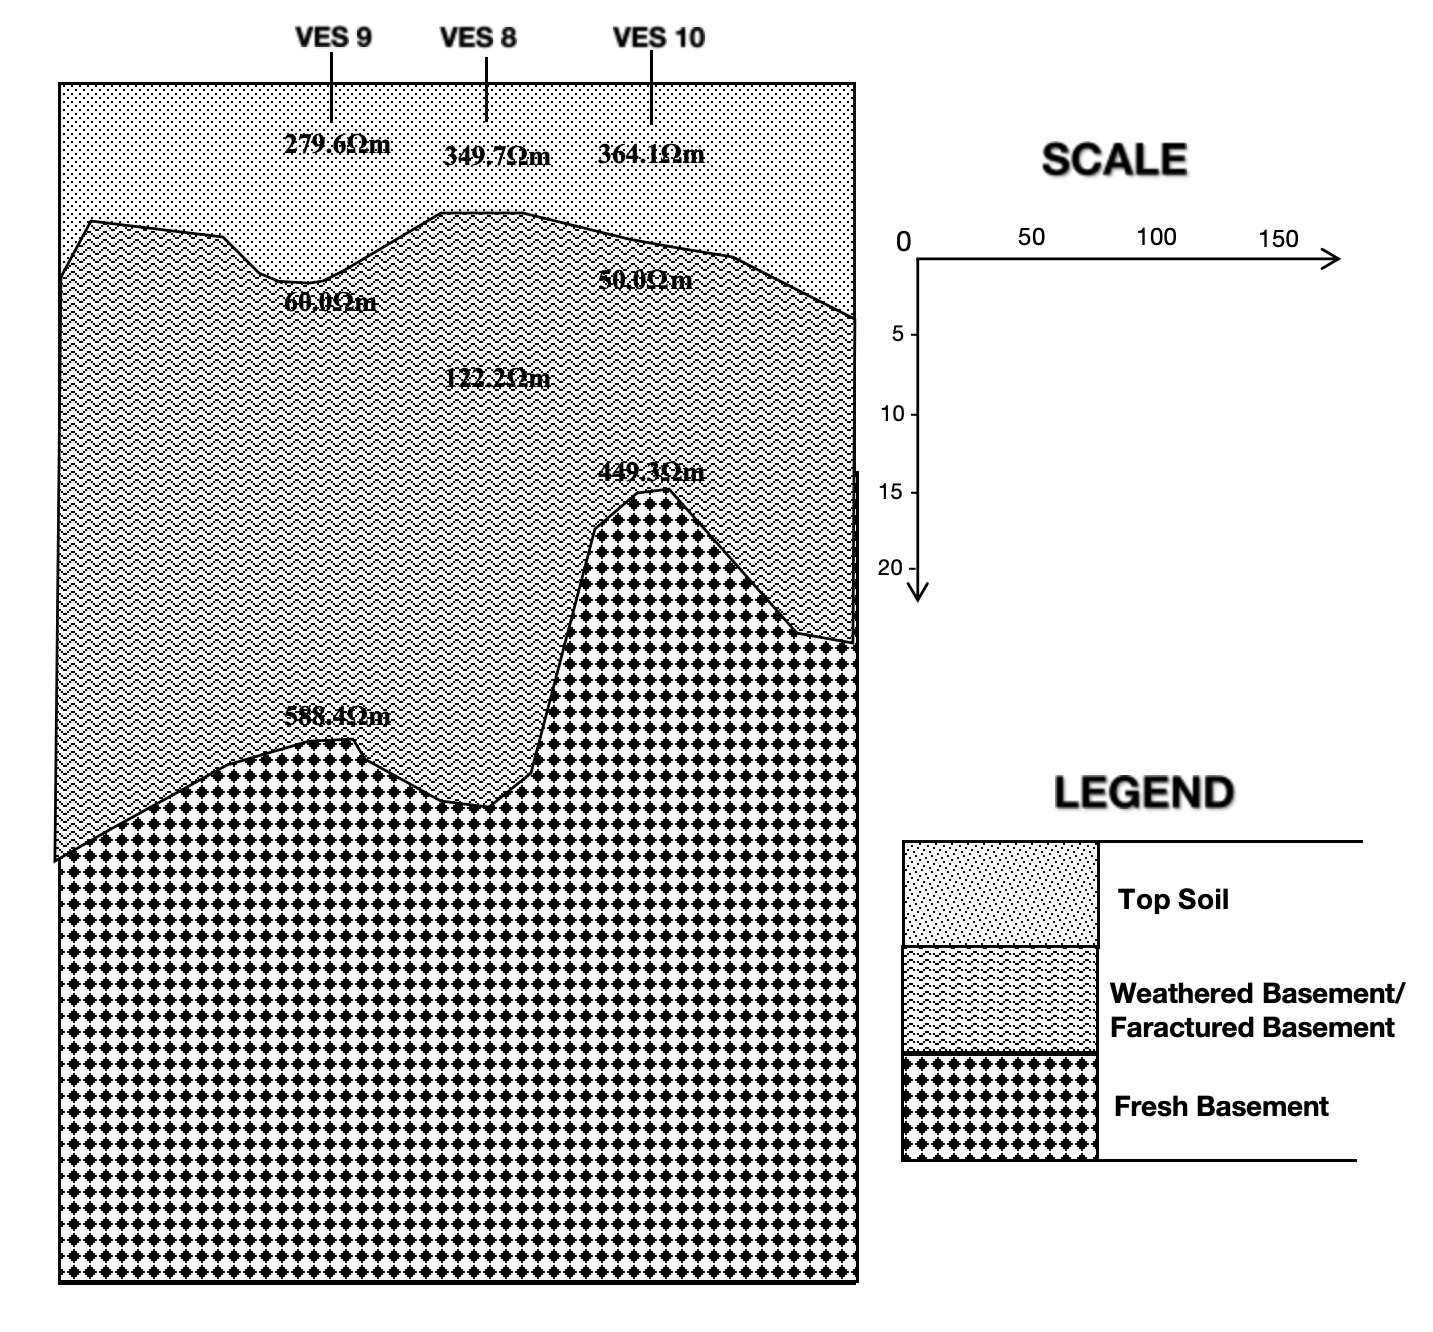
\includegraphics[width=1.0\textwidth]{UI_Mosque_Profile1.png}
    \caption{Geoelectric Section along Profile 1 at UI Mosque using Surfer}
    \label{fig:UI_Mosque_Surfer_Profile_1}
\end{figure}

\subsection{UI Mosque Profile 2 Geoelectric Section}
\begin{figure}[H]
    \centering
    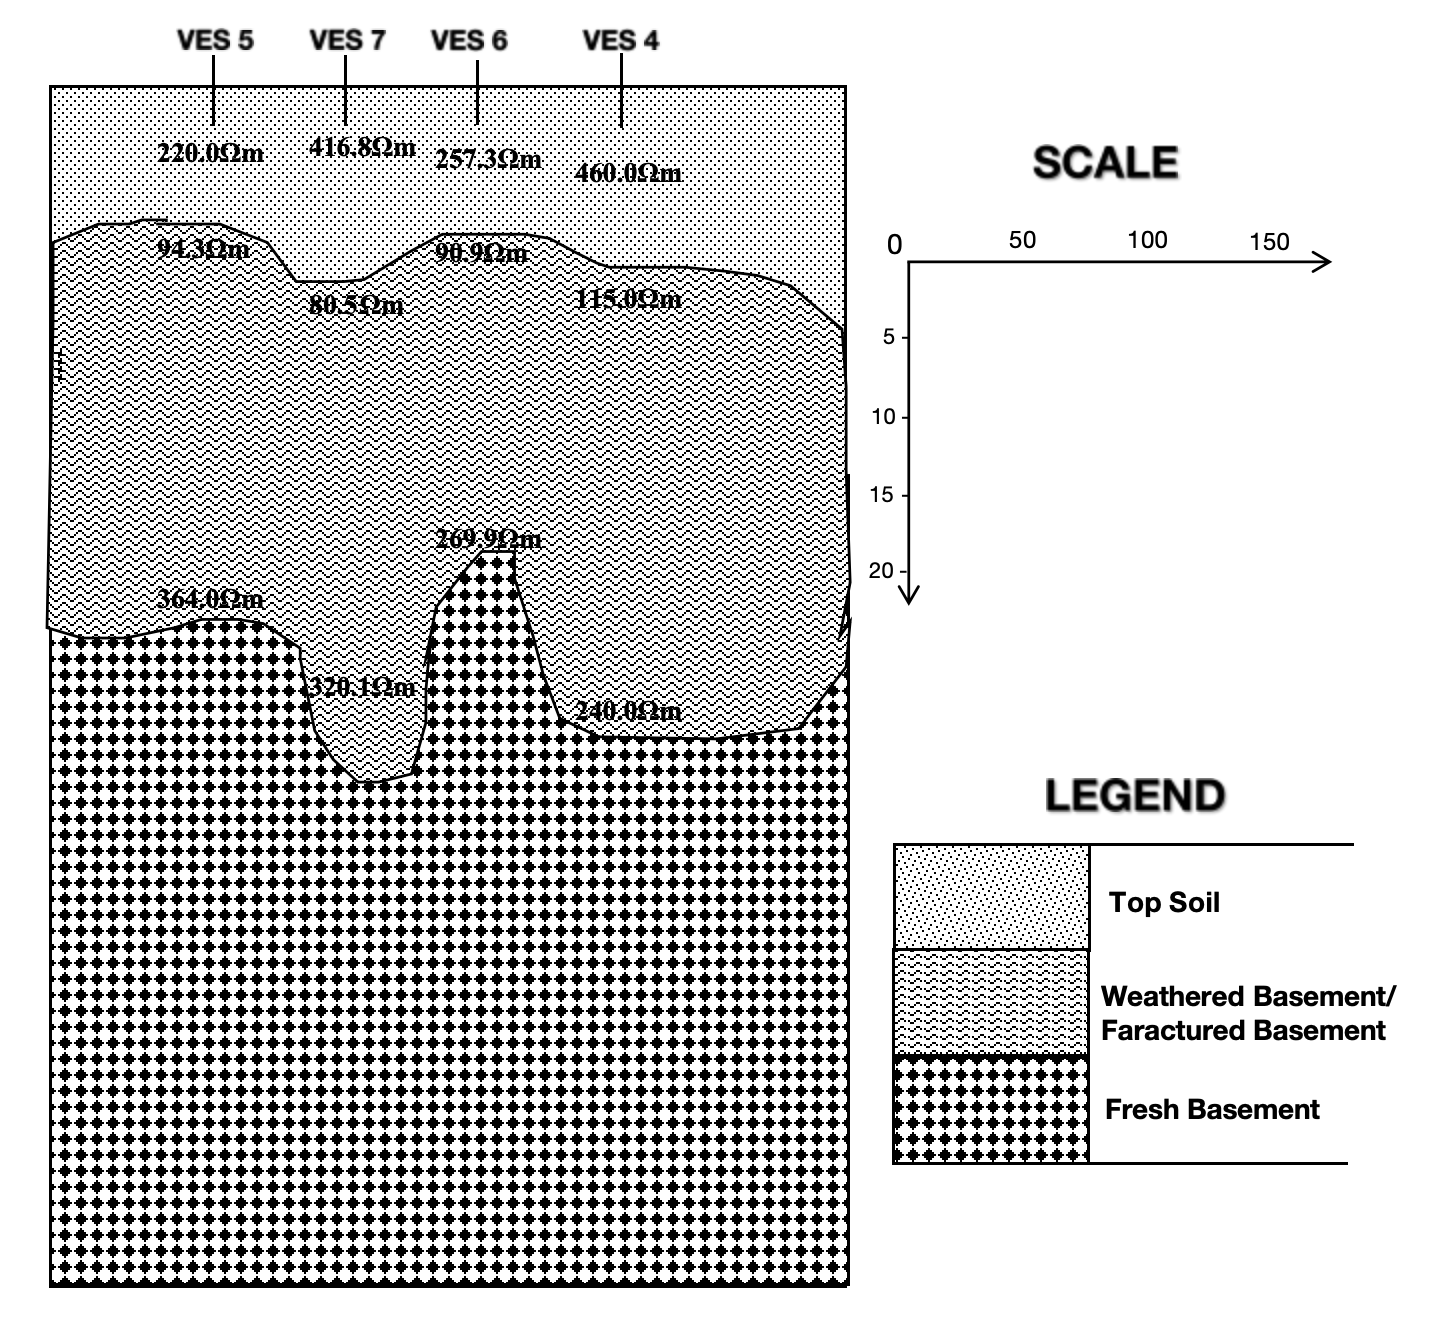
\includegraphics[width=1.0\textwidth]{UI_Mosque_Profile2.png}
    \caption{Geoelectric Section along Profile 2 at UI Mosque using Surfer}
    \label{fig:UI_Mosque_Surfer_Profile_2}
\end{figure}

\subsection{UI Mosque Profile 3 Geoelectric Section}
\begin{figure}[H]
    \centering
    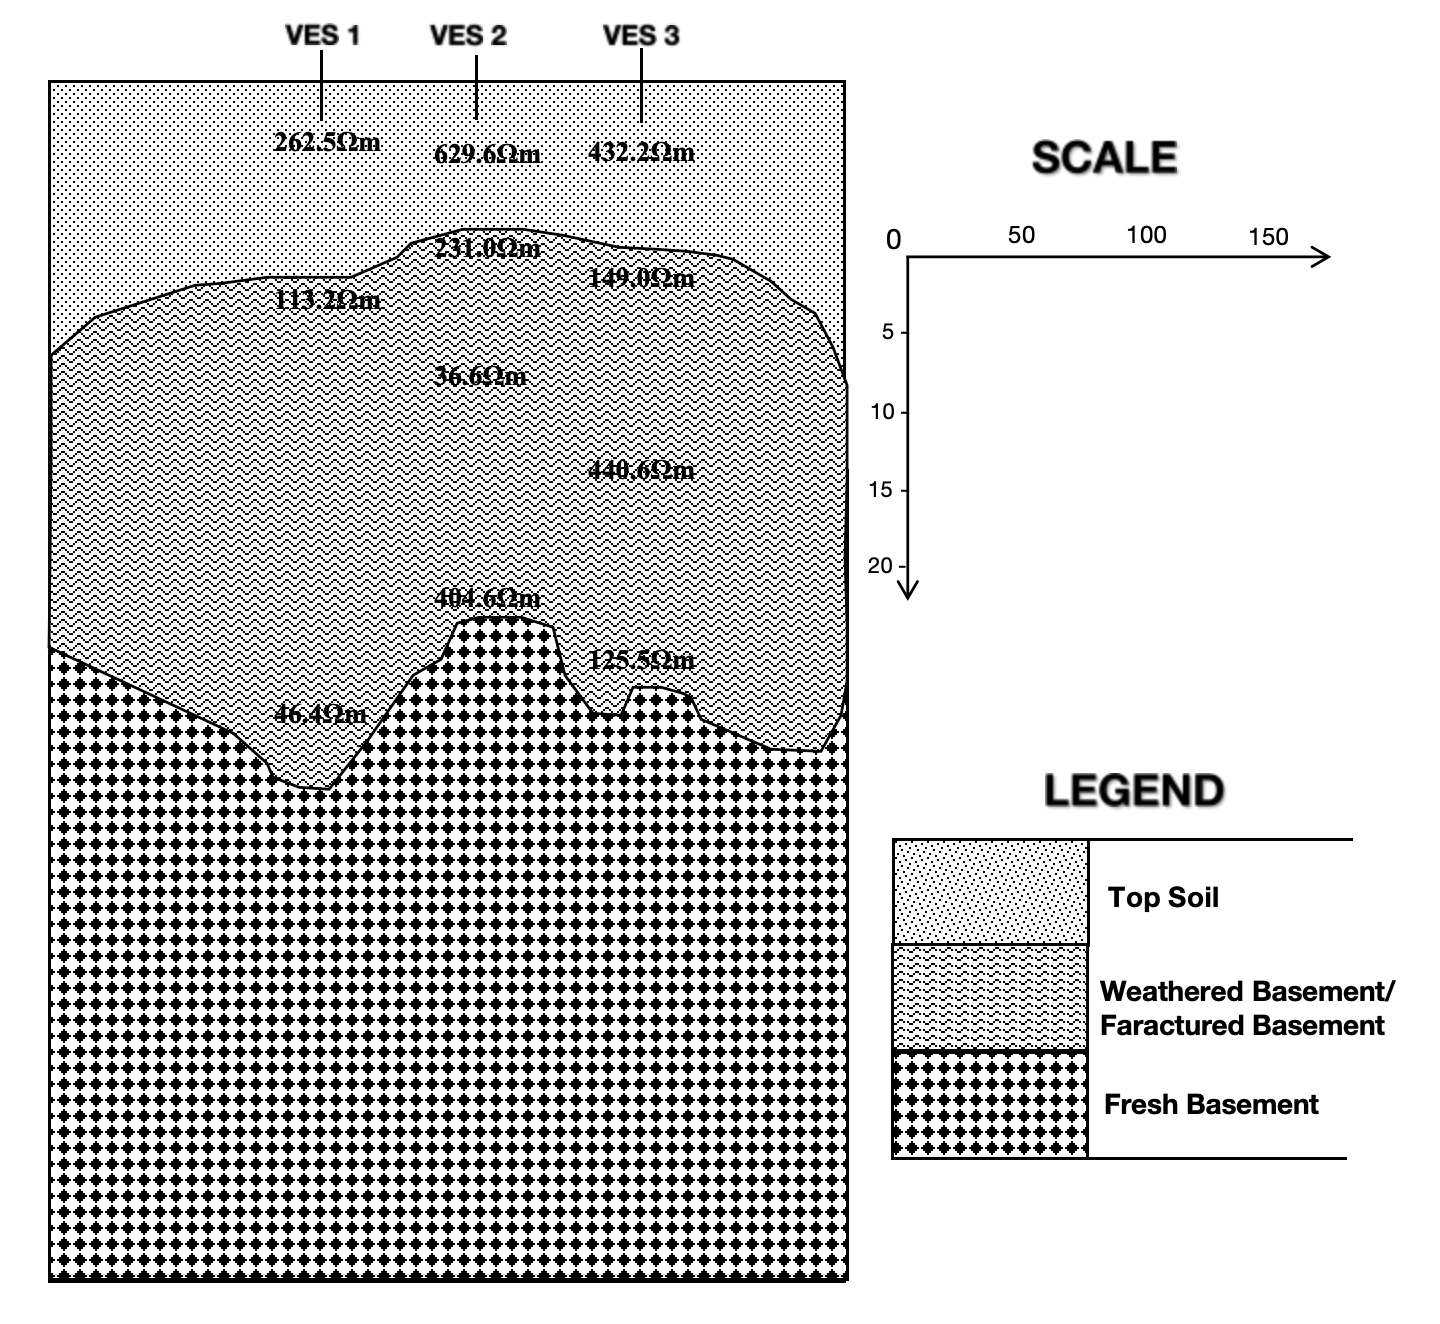
\includegraphics[width=1.0\textwidth]{UI_Mosque_Profile3.png}
    \caption{Geoelectric Section along Profile 3 at UI Mosque using Surfer}
    \label{fig:UI_Mosque_Surfer_Profile_3}
\end{figure}

\subsection{Abubakar Abdulsalam Hall Profile 1 Geoelectric Section}
\begin{figure}[H]
    \centering
    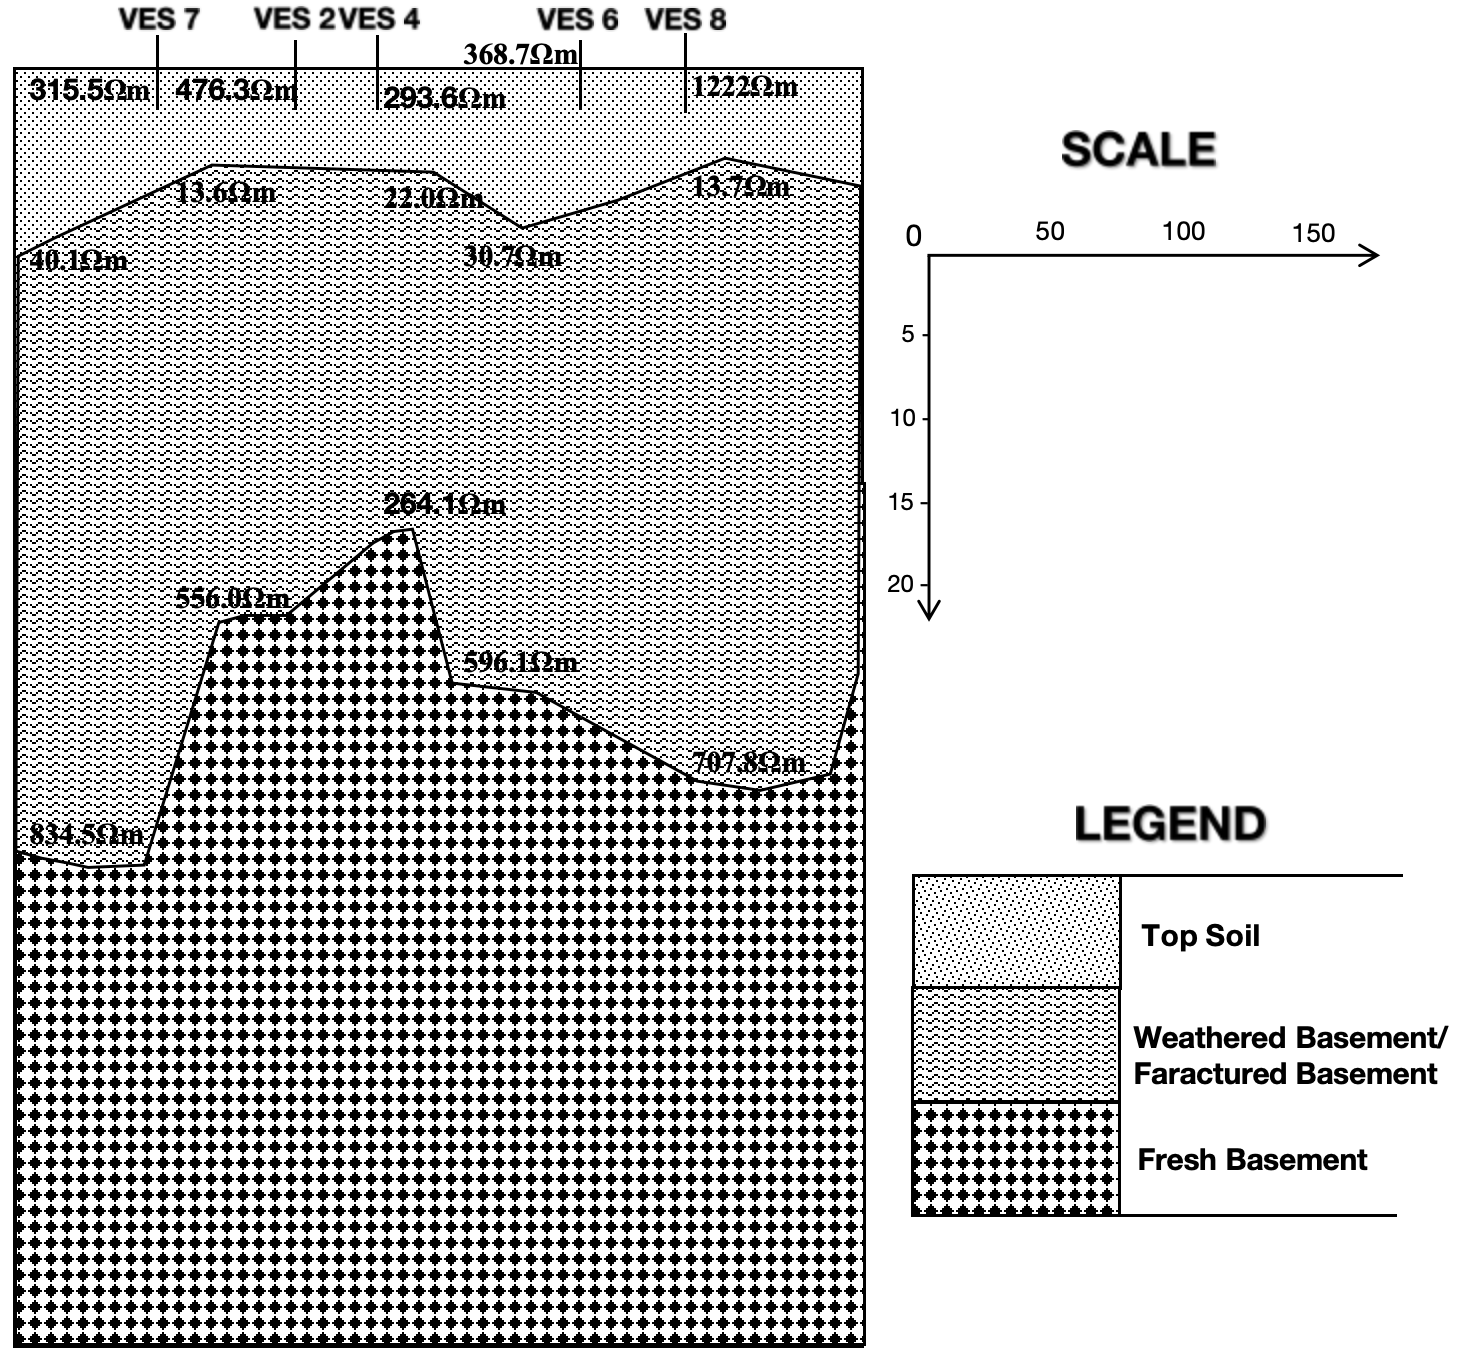
\includegraphics[width=1.0\textwidth]{AAH_PROFILE_1.png}
    \caption{Geoelectric Section along Profile 1 at AAH using Surfer}
    \label{fig:AAH_Surfer_Profile_1}
\end{figure}

\subsection{Abubakar Abdulsalam Hall Profile 1 Geoelectric Section}

\begin{figure}[H]
    \centering
    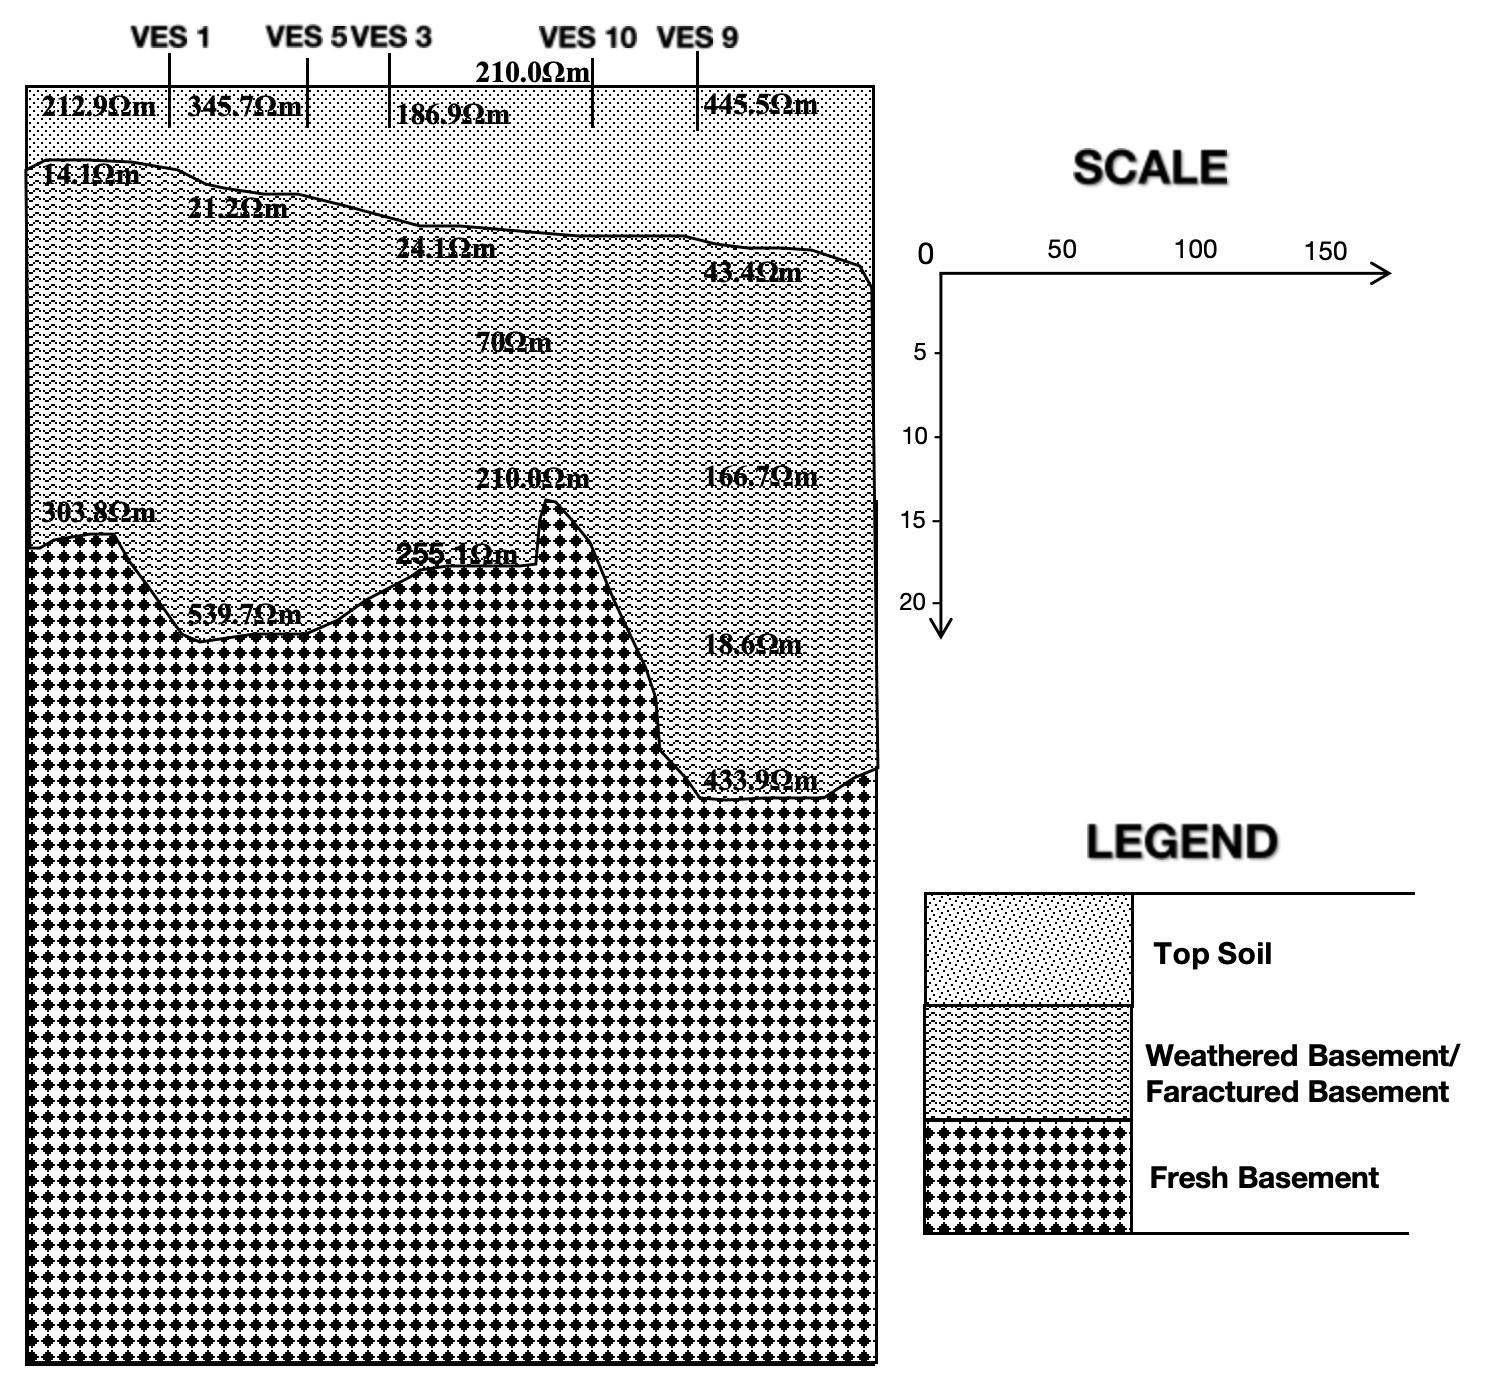
\includegraphics[width=1.0\textwidth]{AAH_PROFILE_2.png}
    \caption{Geoelectric Section along Profile 2 at AAH using Surfer}
    \label{fig:AAH_Surfer_Profile_2}
\end{figure}

\section{Geoelectric Parameters and the Inferred Lithology of the Study Area}
The Electrical Sounding curves from the interpreted results obtained in the previous section in both study areas shown that the two area underlain by three distinct layers in all parts. The Tables below gives the summary of the geoelectric parameters and the model interpretation of the layers. 

\subsection{Model Interpretation of Layers for UI Mosque Study Area}

\begin{longtable}{|>{\raggedright\arraybackslash}m{1.5cm}|>{\raggedright\arraybackslash}m{3cm}|>{\raggedright\arraybackslash}m{3cm}|>{\raggedright\arraybackslash}m{3cm}|>{\raggedright\arraybackslash}m{3cm}|>{\raggedright\arraybackslash}m{1.5cm}|}
    \hline
    \textbf{VES} & \multicolumn{4}{|c|}{\textbf{Geoelectric Parameters}} & \textbf{Curve Type} \\
    \cline{2-5}
     & \textbf{Possible Lithology} & \textbf{Resistivity ($\Omega$m)} & \textbf{Thickness (m)} & \textbf{Depth (m)} &  \\[0.3cm]
    \hline
    \endfirsthead
    \hline
    \textbf{VES} & \multicolumn{4}{|c|}{\textbf{Geoelectric Parameters}} & \textbf{Curve Type} \\
    \cline{2-5}
     & \textbf{Possible Lithology} & \textbf{Resistivity ($\Omega$m)} & \textbf{Thickness (m)} & \textbf{Depth (m)} &  \\[0.3cm]
    \hline
    \endhead
    \hline
    \endfoot
    \hline
    \endlastfoot
        VES 1 & Topsoil & 262.5 & 1.0 & 1.0 & Q \\[0.3cm] \cline{2-5}
              & Weathered Basement & 113.2 & 3.0 & 4.0 &  \\[0.3cm] \cline{2-5}
              & Fresh bedrock & 46.4 & Undetermined & Undetermined &  \\[0.3cm] \cline{2-5}
        \hline
        VES 2 & Topsoil & 629.6 & 0.8 & 0.8 & QH \\[0.3cm] \cline{2-5}
              & Weathered Basement & 231.0 & 3.5 & 4.3 &  \\[0.3cm] \cline{2-5}
              & Clay-rich soil & 36.6 & 11.6 & 15.9 &  \\[0.3cm] \cline{2-5}
              & Basement Rock & 404.6 & Undetermined & Undetermined &  \\[0.3cm] \cline{2-5}
        \hline
        VES 3 & Topsoil & 432.2 & 1.1 & 1.1 & HQ \\[0.3cm] \cline{2-5}
              & Weathered Basement & 149.0 & 4.4 & 5.4 &  \\[0.3cm] \cline{2-5}
              & Basement Rock & 440.6 & 10.0 & 15.4 &  \\[0.3cm] \cline{2-5}
              & Fresh bedrock & 364.1 & Undetermined & Undetermined &  \\[0.3cm] \cline{2-5}
        \hline
        VES 4 & Topsoil & 460.0 & 1.0 & 1.0 & H \\[0.3cm] \cline{2-5}
              & Weathered Basement & 115.0 & 10.5 & 11.5 &  \\[0.3cm] \cline{2-5}
              & Fresh bedrock & 240.0 & Undetermined & Undetermined &  \\[0.3cm] \cline{2-5}
        \hline
        VES 5 & Topsoil & 220.0 & 1.0 & 1.0 & H \\[0.3cm] \cline{2-5}
              & Weathered Basement & 94.3 & 21 & 22 &  \\[0.3cm] \cline{2-5}
              & Fresh bedrock & 364.0 & Undetermined & Undetermined &  \\[0.3cm] \cline{2-5}
        \hline
        VES 6 & Topsoil & 257.3 & 1.0 & 1.0 & H \\[0.3cm] \cline{2-5}
              & Weathered Basement & 90.9 & 9.0 & 10.0 &  \\[0.3cm] \cline{2-5}
              & Fresh bedrock & 269.9 & Undetermined & Undetermined &  \\[0.3cm] \cline{2-5}
        \hline
        VES 7 & Topsoil & 416.8 & 1.1 & 1.1 & H \\[0.3cm] \cline{2-5}
              & Weathered Basement & 80.5 & 10.1 & 11.6 &  \\[0.3cm] \cline{2-5}
              & Fresh bedrock & 320.1 & Undetermined & Undetermined &  \\[0.3cm] \cline{2-5}
        \hline
        VES 8 & Topsoil & 349.7 & 1.0 & 1.0 & Q \\[0.3cm] \cline{2-5}
              & Weathered Basement & 122.2 & 6.6 & 7.6 &  \\[0.3cm] \cline{2-5}
              & Fresh bedrock & 27.7 & Undetermined & Undetermined &  \\[0.3cm] \cline{2-5}
        \hline
        VES 9 & Topsoil & 279.6 & 1.1 & 1.1 & H \\[0.3cm] \cline{2-5}
              & Weathered Basement & 60.0 & 18.8 & 20.0 &  \\[0.3cm] \cline{2-5}
              & Fresh bedrock & 588.4 & Undetermined & Undetermined &  \\[0.3cm] \cline{2-5}
        \hline
        VES 10 & Topsoil & 364.1 & 0.9 & 0.9 & H \\[0.3cm] \cline{2-5}
              & Weathered Basement & 50.0 & 10.8 & 11.7 &  \\[0.3cm] \cline{2-5}
              & Fresh bedrock & 449.3 & Undetermined & Undetermined &  \\[0.3cm] \cline{2-5}
        \hline
        \caption{Interpretation of Layers at UI Mosque Study Area}
        \label{tab:ui_study_layer}
\end{longtable}

\subsection{Model Interpretation of Layers for AAH Study Area}

\begin{longtable}{|>{\raggedright\arraybackslash}m{1.5cm}|>{\raggedright\arraybackslash}m{3.5cm}|>{\raggedright\arraybackslash}m{2.5cm}|>{\raggedright\arraybackslash}m{3cm}|>{\raggedright\arraybackslash}m{3cm}|>{\raggedright\arraybackslash}m{1.5cm}|}
    \hline
    \textbf{VES} & \multicolumn{4}{|c|}{\textbf{Geoelectric Parameters}} & \textbf{Curve Type} \\
    \cline{2-5}
     & \textbf{Possible Lithology} & \textbf{Resistivity ($\Omega$m)} & \textbf{Thickness (m)} & \textbf{Depth (m)} &  \\[0.3cm]
    \hline
    \endfirsthead
    \hline
    \textbf{VES} & \multicolumn{4}{|c|}{\textbf{Geoelectric Parameters}} & \textbf{Curve Type} \\
    \cline{2-5}
     & \textbf{Possible Lithology} & \textbf{Resistivity ($\Omega$m)} & \textbf{Thickness (m)} & \textbf{Depth (m)} &  \\[0.3cm]
    \hline
    \endhead
    \hline
    \endfoot
    \hline
    \endlastfoot
        VES 1 & Topsoil & 212.9 & 1.0 & 1.0 & H \\[0.3cm] \cline{2-5}
              & Weathered Basement & 141.1 & 8.3 & 9.3 &  \\[0.3cm] \cline{2-5}
              & Fresh bedrock & 303.8 & Undetermined & Undetermined &  \\[0.3cm] \cline{2-5}
        \hline
        VES 2 & Topsoil & 476.3 & 0.8 & 0.8 & H \\[0.3cm] \cline{2-5}
              & Weathered Basement & 13.6 & 3.0 & 3.8 &  \\[0.3cm] \cline{2-5}
              & Fresh bedrock & 556.0 & Undetermined & Undetermined &  \\[0.3cm] \cline{2-5}
        \hline
        VES 3 & Topsoil & 186.9 & 1.0 & 1.0 & H \\[0.3cm] \cline{2-5}
              & Weathered Basement & 24.1 & 5.3 & 6.3 &  \\[0.3cm] \cline{2-5}
              & Fresh bedrock & 255.1 & Undetermined & Undetermined &  \\[0.3cm] \cline{2-5}
        \hline
        VES 4 & Topsoil & 293.6 & 0.8 & 0.8 & H \\[0.3cm] \cline{2-5}
              & Weathered Basement & 22.0 & 4.7 & 5.5 &  \\[0.3cm] \cline{2-5}
              & Fresh bedrock & 264.1 & Undetermined & Undetermined &  \\[0.3cm] \cline{2-5}
        \hline
        VES 5 & Topsoil & 345.7 & 0.8 & 0.8 & H \\[0.3cm] \cline{2-5}
              & Weathered Basement & 21.2 & 4.3 & 5.1 &  \\[0.3cm] \cline{2-5}
              & Fresh bedrock & 539.7 & Undetermined & Undetermined &  \\[0.3cm] \cline{2-5}
        \hline
        VES 6 & Topsoil & 368.7 & 0.8 & 0.8 & H \\[0.3cm] \cline{2-5}
              & Weathered Basement & 30.7 & 8.2 & 8.9 &  \\[0.3cm] \cline{2-5}
              & Fresh bedrock & 596.1 & Undetermined & Undetermined &  \\[0.3cm] \cline{2-5}
        \hline
        VES 7 & Topsoil & 315.5 & 1.0 & 1.0 & H \\[0.3cm] \cline{2-5}
              & Weathered Basement & 40.1 & 9.9 & 10.9 &  \\[0.3cm] \cline{2-5}
              & Fresh bedrock & 834.5 & Undetermined & Undetermined &  \\[0.3cm] \cline{2-5}
        \hline
        VES 8 & Topsoil & 1222.0 & 1.0 & 1.0 & H \\[0.3cm] \cline{2-5}
              & Weathered Basement & 13.7 & 2.6 & 3.6 &  \\[0.3cm] \cline{2-5}
              & Fresh bedrock & 707.8 & Undetermined & Undetermined &  \\[0.3cm] \cline{2-5}
        \hline
        VES 9 & Topsoil & 445.4 & 0.5 & 0.5 & KHK \\[0.3cm] \cline{2-5}
              & Clay or water-saturated & 43.4 & 1.4 & 1.9 &  \\[0.3cm] \cline{2-5}
              & Compacted Rock / unsaturated sandstone & 166.7 & 11.4 & 13.2 &  \\[0.3cm] \cline{2-5}
              & High Conductive (water-saturated) & 18.6 & 3.8 & 17.0 &  \\[0.3cm] \cline{2-5}
              & Fresh bedrock & 433.9 & Undetermined & Undetermined &  \\[0.3cm] \cline{2-5}
        \hline
        VES 10 & Topsoil & 210.0 & 0.7 & 0.7 & H \\[0.3cm] \cline{2-5}
              & Weathered Basement & 70.0 & 4.8 & 5.5 &  \\[0.3cm] \cline{2-5}
              & Fresh bedrock & 210.0 & Undetermined & Undetermined &  \\[0.3cm] \cline{2-5}
        \hline
        \caption{Interpretation of Layers at AAH Study Area}
        \label{tab:aah_study_layer}
\end{longtable}

\chapter{CHAPTER 5: SUMMARY, CONCLUSION, AND RECOMMENDATIONS}

\section{SUMMARY}

This project explored the application of electrical resistivity methods, including Vertical Electrical Sounding (VES) and Constant Separation Traversing (CST), to investigate subsurface characteristics for geophysical purposes. The project emphasized the integration of field data acquisition, processing, and interpretation techniques to develop resistivity models that provide insights into subsurface lithology and structural anomalies.

The methodology employed standard configurations such as Schlumberger for depth-specific studies and Wenner for horizontal resistivity variations, leveraging their strengths in capturing diverse geophysical features. The data acquisition process involved systematic profiling of the study area, with rigorous calibration and correction techniques applied to ensure accuracy. Advanced software tools, such as WINRESIST and DIPROWIN, were utilized to process and invert apparent resistivity values into true resistivity models, revealing detailed curves for VES and 2D subsurface images for CST.

This project underscores the importance of geoelectrical techniques as cost-effective, non-invasive tools for subsurface investigations, contributing to resource exploration, environmental studies, and civil engineering projects.

\section{RECOMMENDATIONS}

Based on the findings and observations from this project, the following recommendations are proposed:

\begin{enumerate}
    \item \textbf{Adoption of Multi-Method Approaches:} To address the inherent limitations of resistivity methods, future investigations should combine electrical resistivity with complementary geophysical techniques such as seismic refraction or ground-penetrating radar. This integrated approach will improve the resolution and reliability of subsurface models.
    
    \item \textbf{Enhanced Data Acquisition Strategies:} Future surveys should prioritize denser electrode spacing and extended profiles to capture more detailed resistivity variations. This is particularly important in areas with complex geology or high groundwater potential.
    
    \item \textbf{Use of Advanced Inversion Techniques:} Leveraging emerging algorithms and 3D inversion software can enhance the accuracy and interpretability of resistivity data. Researchers should also consider the use of machine learning and artificial intelligence tools for automated data analysis and pattern recognition.
    
    \item \textbf{Environmental Monitoring and Adaptation:} Environmental factors such as soil moisture, temperature, and anthropogenic interference significantly influence resistivity measurements. Efforts should be made to monitor and compensate for these variables during data acquisition and processing.
    
    \item \textbf{Capacity Building and Training:} Continuous training of geophysicists and engineers in the latest resistivity technologies and software tools is essential to ensure the effective implementation of geophysical surveys. Workshops, certifications, and collaborations with research institutions can enhance expertise in the field.
     
    \item \textbf{Further Research:} Future studies should focus on improving resistivity interpretation by conducting controlled field experiments in well-characterized areas. These studies can help refine resistivity models and develop standardized protocols for subsurface investigations.
\end{enumerate}

By addressing these recommendations, the reliability and applicability of electrical resistivity methods can be significantly enhanced, paving the way for more impactful contributions to geology, hydrology, and engineering.

\section{CONCLUSION}

The project demonstrated the use of electrical resistivity methods in delineating subsurface structures within the study areas. The Schlumberger and Wenner configurations proved to be complementary techniques, effectively capturing vertical and lateral resistivity variations, respectively.

By applying practical curve matching techniques and employing advance software tools, the study produced high-resolution resistivity profiles that provided critical insights into subsurface conditions. The results confirmed the presence of lithological boundaries, aquiferous zones, and potential weak structural areas, validating the reliability of the adopted geophysical methods.

While this project achieved its objectives, it also revealed the limitations of geoelectrical methods, particularly their sensitivity to environmental factors and the inherent ambiguities in resistivity interpretation. Addressing these limitations through the recommendations like multi-method integration and advanced processing techniques will further enhance the reliability of subsurface investigations.

\chapter*{REFFERENCES}
\addcontentsline{toc}{chapter}{REFFERENCES}
\begin{justify}
    Abiola, O. (2024). Geophysical Evaluation of Subsurface Competence in Parts of the Senior Staff Quarters of the Federal University of Technology, Akure, Nigeria. A Publication of the Centre for Research and Development (CERAD). \\

    Adagunodo, T. A., Sunmonu, L. A., Salako, K. A. (2013). Geophysical investigation into the cause of structural failure in a building at Ogbomoso, Southwestern Nigeria. IOSR Journal of Applied Physics, 3(4), 08-16. \\
    
    Adetoyinbo, A. A., Bello, A. K., Magi, F. F. (2023). Subsurface Characteristics and Evaluation of Groundwater Potential Zone of Idi-Ayunre, Southwest, Nigeria. International Journal of Science Academic Research, 4(6), 5714-5721. \\
    
    Adeyemi, G. O., Bello, A. A. (2020). Geophysical and hydrogeological investigation of groundwater potential in part of Lagos State, Southwestern Nigeria. Journal of Applied Sciences and Environmental Management, 24(1), 57-63. \\
    
    Agada, P. O., Ibuot, J. C., Oseghale, A. D. (2013). Geoelectrical investigation of groundwater potential in Emohua LGA, Rivers State, Nigeria. International Journal of Scientific Engineering Research, 4(9), 1745-1751. \\
    
    Akintoye, A. E., Olorunfemi, M. O., Ojo, J. S. (2018). Geoelectrical investigation of groundwater potential and aquifer vulnerability in a typical basement complex environment: A case study of Ado-Ekiti, Southwestern Nigeria. Nigerian Journal of Technological Development, 15(1), 1-10. \\
    
    Amadi, A., et al. (2012). Architect's and Geologist's View on the Causes of Building Failures in Nigeria. Modern Applied Science, 6(6), 31. \\
    
    Anomohanran, O. (2013). Seismic refraction method: A technique for determining the thickness of stratified substratum. American Journal of Applied Sciences, 10(8), 857-863. \\
    
    Barker, R. D. (1980). Application of Geophysics in Groundwater Investigations. Water Survey, 84, 489-492. \\
    
    Bermúdez, M. A., González-Serna, J. M., Martín-Crespo, T. (2020). Application of electrical resistivity tomography to the detection of subsurface cavities. \\
    
    Binley, A. (2015). Tools and Techniques: Electrical Methods. In G. Schubert (Ed.), Treatise on Geophysics (Vol. 11, pp. 233-259). Cambridge, MA: Elsevier Science. doi:10.1016/B978-0-444-53802-4.00192-5. \\
    
    Coker, J. O. (2012). Geoelectrical investigation of groundwater potential in Mubi, Adamawa State, Nigeria. Journal of Geology and Mining Research, 4(2), 35-40. \\
    
    Emilio, M., Riccardi, U. (2010). Geophysical methods applied to engineering and environmental problems. Springer, 1-10. \\
    
    Eze, C. L., Ugwu, S. A., Okoye, C. O. (2017). Geoelectrical investigation of groundwater potential in Enugu State, Southeastern Nigeria. Journal of Earth System Science, 126(5), 68. \\
    
    Fadillah, T., Gross, L., Schaa, R. (2018). Estimation of Aquifer Properties Using Surface-Based Electrical Resistivity Tomography. doi:10.3997/2214-4609.201800374. \\
    
    Farinde, O. A., Enikanselu, P. A. (2015). Geophysical investigation of road pavement instability along Ibadan–Ife Expressway, Southwestern Nigeria. Journal of Applied Geology and Geophysics, 3(1), 01-09. \\
    
    Griffiths, D. H., Barker, R. D. (1993). Two-dimensional resistivity imaging and modeling in areas of complex geology. Journal of Applied Geophysics, 29(3-4), 211-226. \\
    
    Ismaila, A. A., Akanbi, E. S. (2019). Geophysical investigation of groundwater potential in part of Ilorin, Southwestern Nigeria. Nigerian Journal of Technological Development, 16(1), 1-8. \\
    
    James, D. A., Olatunji, S. O. (2019). Geophysical investigation of groundwater potential in part of Ibadan metropolis, Southwestern Nigeria. Journal of Applied Sciences and Environmental Management, 23(2), 311-316. \\
    
    Kunetz, G. (1966). Principles of Direct Current Resistivity Prospecting. Gebrüder Borntraeger. \\
    
    Kværno, S. H., Øygarden, L. (2006). The Influence of Freeze-Thaw Cycles and Soil Moisture on Aggregate Stability of Three Soils in Norway. Catena, 67(3), 175-182. \\
    
    Lapenna, V., Lorenzo, P., Perrone, A., Piscitelli, S., Rizzo, E., Sdao, F. (2005). 2D electrical resistivity imaging of some complex landslides in the Lucanian Apennine chain, southern Italy. Geophysics, 70(3), B11-B18. \\
    
    Loke, M. H. (2016). Tutorial: 2-D and 3-D electrical imaging surveys. Geotomo Software, Malaysia. \\
    
    Mosuro, G. O., Omosanya, K. O., Bayewu, O. O., Oloruntola, M. O., Laniyan, T. A., Atobi, O., Okubena, M., Popoola, E. (2017). Assessment of Groundwater Vulnerability to Leachate Infiltration Using Electrical Resistivity Method. Applied Water Science, 7(5), 2195-2207. doi:10.1007/s13201-016-0393-4. \\
    
    Ogunseye, T. T., Bello, A. K., Ozegin, K. O., Akpotor, J. N. (2022). Geochemical Soil Analysis for Groundwater Quality at Mokola Area, Ibadan, Southwestern Nigeria. IOSR Journal of Applied Geology and Geophysics. \\
    
    Olayemi, O. M., Ojo, J. S., Olorunfemi, M. O. (2021). Geoelectrical assessment of groundwater potential in a typical basement complex terrain: A case study of Iwaraja, Southwestern Nigeria. Nigerian Journal of Technological Development, 18(1), 1-9. \\
    
    Ozevin, D., Dindarloo, S. R. (2017). Acoustic emission monitoring of corrosion in prestressed concrete structures. Journal of Materials in Civil Engineering, 29(10), 04017193. \\
    
    Reynolds, J. M. (2011). An Introduction to Applied and Environmental Geophysics (2nd ed.). Wiley-Blackwell. \\
    
    Sharma, P. V. (1986). Geophysical Methods in Geology (2nd ed.). Elsevier. \\
    
    Soupios, P., Papazachos, C., Sarris, A., Vallianatos, F., Makris, J., Vafidis, A. (2006). Estimation of aquifer parameters from surficial geophysical methods: A case study of Keritis Basin in Crete. Journal of Hydrology, 338(1-2), 122-131. \\
    
    Steeples, D. W., Chilton, J. (2001). Groundwater exploration using seismic refraction and electrical resistivity methods in a karst area of southeastern Minnesota. Geophysics, 66(2), 482-489. \\
    
    Telford, W. M., Geldart, L. P., Sheriff, R. E. (1990). Applied Geophysics (2nd ed.). Cambridge University Press. \\
    
    Warner, M. (2004). Seismic reflection inversion: Methods, pitfalls, and applications. European Association of Geoscientists Engineers, 22(5), 123-136. \\

    Zohdy, A.A.R. (1973). A Computer Program for Automatic Interpretation of Schlumberger Sounding Curves over Horizontally Stratified Media. PB-232703, National Technical Information Service, Springfield, Virginia, 25 p. \\
\end{justify}

\textbf{Image Source:} \\

\begin{enumerate}  
    \item \textbf{Figure 2.1} \href{https://www.researchgate.net/figure/Diagram-illustrating-electrical-current-flow-through-the-subsurface-using-the-Wenner_fig6_372649419}{ResearchGate: Electrical Current Flow}
    \item \textbf{Figure 2.2} \href{https://www.researchgate.net/figure/Simplified-current-flow-lines-and-equipotential-surfaces-arising-from-a-a-single_fig1_323353321}{ResearchGate: Current Flow Lines}
    \item \textbf{Figure 2.3} \href{https://www.researchgate.net/figure/Apparent-resistivity-curve-for-a-two-layer-model_fig3_336309181}{ResearchGate: Apparent Resistivity Curve}
    \item \textbf{Figure 2.4 (a)} \href{https://www.researchgate.net/figure/Schematic-diagram-of-the-schlumberger-array-used-in-the-survey_fig3_332030886https://www.researchgate.net/figure/Schematic-diagram-of-the-schlumberger-array-used-in-the-survey_fig3_332030886}{Schlumberger array electrode configurations.}
    \item \textbf{Figure 2.4 (b)} \href{https://www.researchgate.net/figure/Wenner-array-a-is-electrode-spacing-and-distribution-of-electric-field-underneath_fig1_238505598}{ResearchGate: Wenner array electrode configurations.}
    \item \textbf{Figure 3.2} \href{https://www.scirp.org/journal/paperinformation?paperid=8137}{SCIRP: Paper Information}
    \item \textbf{Figure 4.1} \href{https://www.slideshare.net/slideshow/resistivity-survey/91069642}{SlideShare: Resistivity Survey}
\end{enumerate}

\chapter*{ACRONYMS}
\addcontentsline{toc}{chapter}{ACRONYMS}

\textbf{AAH} \textendash{} Abubakar Abdulsalam Hall \\ [0.5cm]
\textbf{UI} \textendash{} University of Ibadan \\ [0.5cm]
\textbf{QGIS} \textendash{} Quantum Geographic Information System \\ [0.5cm]
\textbf{VES} \textendash{} Vertical Electrical Sounding \\ [0.5cm]
\textbf{CST} \textendash{} Constant Separation Traversing \\ [0.5cm]
\textbf{ERT} \textendash{} Electrical Resistivity Tomography \\ [0.5cm]
\textbf{Surfer} \textendash{} A software program that helps to create 2D and 3D models of from geospatial data \\ [0.5cm]
\textbf{WINRESIST} \textendash{} A software program that creates one-dimensional 1D electrical resistivity models \\ [0.5cm]
\textbf{DIPROWIN} \textendash{} A software program that creates two-dimensional 2D electrical resistivity models

\end{document}
